%%%%%%%% ICML 2025 EXAMPLE LATEX SUBMISSION FILE %%%%%%%%%%%%%%%%%

\documentclass{article}

% Recommended, but optional, packages for figures and better typesetting:
\usepackage{microtype}
\usepackage{graphicx}
\usepackage{subfigure}
\usepackage{booktabs} % for professional tables
\usepackage{tabularx}
\usepackage{multirow}
\usepackage{amssymb} % for checkmark symbol

% hyperref makes hyperlinks in the resulting PDF.
% If your build breaks (sometimes temporarily if a hyperlink spans a page)
% please comment out the following usepackage line and replace
% \usepackage{icml2025} with \usepackage[nohyperref]{icml2025} above.
\usepackage{hyperref}

% Attempt to make hyperref and algorithmic work together better:
\newcommand{\theHalgorithm}{\arabic{algorithm}}

% Use the following line for the initial blind version submitted for review:
% \usepackage{icml2025}

% If accepted, instead use the following line for the camera-ready submission:
\usepackage[preprint]{icml2025}
% \usepackage[accepted]{icml2025}

% For theorems and such
\usepackage{amsmath}
\usepackage{amsthm}

% if you use cleveref..
\usepackage[capitalize,noabbrev]{cleveref}
\usepackage[most]{tcolorbox} % Load with the 'most' library for additional features
\newtcolorbox{insights}[1][]{%
    colback=blue!5!white, % Light blue background color of the box
    colframe=blue!75!black, % Darker blue border color of the box
    sharp corners, % Makes the corners of the box sharp
    toprule=0pt, % Remove top border
    bottomrule=0pt, % Remove bottom border
    leftrule=1.2pt, % Keep left border
    rightrule=1.2pt, % Keep right border
    #1 % Additional options
}
% \newtcolorbox{insights}[1][]{%
%     colback=#0164E0!5!white, % Light Llama blue background color
%     colframe=#0164E0!75!black, % Darker Llama blue border color
%     sharp corners, % Makes the corners of the box sharp
%     boxrule=1.2pt, % Thickness of the border
%     #1 % Additional options
% }
% \newtcolorbox{insights}[1][]{%
%     colback=#76B900!5!white, % Light NVIDIA green background color
%     colframe=#76B900!75!black, % Darker NVIDIA green border color
%     sharp corners, % Makes the corners of the box sharp
%     boxrule=1.2pt, % Thickness of the border
%     #1 % Additional options
% }

%%%%%%%%%%%%%%%%%%%%%%%%%%%%%%%%
% THEOREMS
%%%%%%%%%%%%%%%%%%%%%%%%%%%%%%%%
\theoremstyle{plain}
\newtheorem{theorem}{Theorem}[section]
\newtheorem{proposition}[theorem]{Proposition}
\newtheorem{lemma}[theorem]{Lemma}
\newtheorem{corollary}[theorem]{Corollary}
\theoremstyle{definition}
\newtheorem{definition}[theorem]{Definition}
\newtheorem{assumption}[theorem]{Assumption}
\theoremstyle{remark}
\newtheorem{remark}[theorem]{Remark}

% Todonotes is useful during development; simply uncomment the next line
%    and comment out the line below the next line to turn off comments
%\usepackage[disable,textsize=tiny]{todonotes}
\usepackage[textsize=tiny]{todonotes}


% The \icmltitle you define below is probably too long as a header.
% Therefore, a short form for the running title is supplied here:
\icmltitlerunning{Everyone Can Train Large Language Models with Small Edge Devices}


\begin{document}
\setlength{\parskip}{3pt plus3pt minus3pt}
% 1.2pt:基础段落间距为 1.2 点(约 0.42 毫米)。
% plus3pt:允许 LaTeX 在排版需要时增加最多 3pt 的弹性间距(例如避免页面底部留白过多)。
% minus2.5pt:允许 LaTeX 在排版需要时减少最多 2.5pt 的弹性间距(例如避免内容被截断)。
% \setlength{\textfloatsep}{3pt plus2pt minus2pt} % 顶部/底部浮动体
% \setlength{\intextsep}{3pt plus2pt minus2pt}      % 中间浮动体
% 减少图表与上下文的间距(例如设为 10pt + 弹性值)

% 调整图片标题与内容的间距
% \setlength{\abovecaptionskip}{-10pt}  % 标题上方间距
% \setlength{\belowcaptionskip}{-10pt}   % 标题下方间距

% % 调整表格标题与内容的间距(表格标题通常在表格上方)
% \setlength{\abovecaptionskip}{-10pt}   % 表格标题上方间距
% \setlength{\belowcaptionskip}{-10pt}   % 表格标题下方间距


\twocolumn[
% \icmltitle{Position: Will LLMs Scaling Hit the Wall? Breaking Barriers with Distributed Resources on Massive Edge Devices}
\icmltitle{Will LLMs Scaling Hit the Wall? Breaking Barriers with Distributed Resources on Massive Edge Devices}
% It is OKAY to include author information, even for blind
% submissions: the style file will automatically remove it for you
% unless you've provided the [accepted] option to the icml2025
% package.

% List of affiliations: The first argument should be a (short)
% identifier you will use later to specify author affiliations
% Academic affiliations should list Department, University, City, Region, Country
% Industry affiliations should list Company, City, Region, Country

% You can specify symbols, otherwise they are numbered in order.
% Ideally, you should not use this facility. Affiliations will be numbered
% in order of appearance and this is the preferred way.
\icmlsetsymbol{equal}{*}

\begin{icmlauthorlist}
\icmlauthor{Tao Shen}{equal,cs}
\icmlauthor{Didi Zhu}{equal,cs}
\icmlauthor{Ziyu Zhao}{equal,cs}
\icmlauthor{Chao Wu}{pa}
\icmlauthor{Fei Wu}{cs}
% \icmlauthor{Firstname6 Lastname6}{sch,yyy,comp}
% \icmlauthor{Firstname7 Lastname7}{comp}
      
    
    
      
    
      
    
    
      
    
%\icmlauthor{}{sch}
% \icmlauthor{Firstname8 Lastname8}{sch}
% \icmlauthor{Firstname8 Lastname8}{yyy,comp}
%\icmlauthor{}{sch}
%\icmlauthor{}{sch}
\end{icmlauthorlist}

\icmlaffiliation{cs}{College of Computer Science and Technology, Zhejiang University, Hangzhou, China}
\icmlaffiliation{pa}{School of Public Affairs and Academy of Social Governance, Zhejiang University, Hangzhou, China}
% \icmlaffiliation{sch}{School of ZZZ, Institute of WWW, Location, Country}
\icmlcorrespondingauthor{Chao Wu}{chao.wu@zju.edu.cn}
\icmlcorrespondingauthor{Fei Wu}{wufei@zju.edu.cn}


% You may provide any keywords that you
% find helpful for describing your paper; these are used to populate
% the "keywords" metadata in the PDF but will not be shown in the document
\icmlkeywords{Machine Learning, ICML}

\vskip 0.3in
]

% this must go after the closing bracket ] following \twocolumn[ ...

% This command actually creates the footnote in the first column
% listing the affiliations and the copyright notice.
% The command takes one argument, which is text to display at the start of the footnote.
% The \icmlEqualContribution command is standard text for equal contribution.
% Remove it (just {}) if you do not need this facility.

%\printAffiliationsAndNotice{}  % leave blank if no need to mention equal contribution
\printAffiliationsAndNotice{\icmlEqualContribution} % otherwise use the standard text.

% 核心问题:为什么要写这篇文章?主要观点是什么?
% 当前AI发展面临什么问题?(数据和算力瓶颈)
% 有什么潜在的解决方案?(分布式小型边缘设备)
% 这个解决方案带来什么机遇?(开启AI新纪元)

\begin{abstract}
The remarkable success of foundation models has been driven by scaling laws, demonstrating that model performance improves predictably with increased \textit{training data} and \textit{model size}. 
However, this scaling trajectory faces two critical challenges: the depletion of high-quality public data, 
% as evidenced by the exhaustion of web-scale text corpora,
and the prohibitive computational power required for larger models, 
which have been monopolized by tech giants. 
These two bottlenecks pose significant obstacles to the further development of AI.
In this position paper, we argue that leveraging massive distributed edge devices can break through these barriers. 
We reveal the vast untapped potential of data and computational resources on massive edge devices, and review recent technical advancements in distributed/federated learning that make this new paradigm viable.
Our analysis suggests that by collaborating on edge devices, everyone can participate in training large language models with small edge devices.
This paradigm shift towards distributed training on edge has the potential to democratize AI development and foster a more inclusive AI community.
\end{abstract}

% 逻辑主线: 通过分析当前大模型发展面临的瓶颈,提出以联邦学习和边缘设备共同训练模型的必要性。

\section{Introduction}
% \begin{insights}
%     \textbf{insights:}
%     \begin{itemize}
%         \item 111
%     \end{itemize}
% \end{insights}
% 1.1 大模型与Scaling Law的驱动力
% \subsection{Foundation Models and the Driving Force of Scaling Laws}
% - 为什么大模型能成功?(Scaling Law如何推动模型性能提升?)
% - Scaling Law依赖的核心是什么?(模型规模和训练数据规模的扩张)
% - 进一步突破Scaling Law需要满足哪些条件?(更广泛的数据与更强的算力)

\textbf{Scaling laws} \citep{kaplan2020scaling,hoffmann2022training} have been fundamental to the remarkable success of foundation models, demonstrating a predictable relationship between performance and the expansion of model parameters and training data. These laws have guided the development of increasingly powerful models, from BERT \citep{devlin2018bert} to GPT-4 \citep{openai2023gpt4}, showing that performance improvements can be achieved through systematic scaling of both model size and training data \citep{brown2020language,chowdhery2022palm}. However, the continued application of these scaling laws requires ever-increasing amounts of data and computational resources, pushing the boundaries of what is currently feasible \citep{patterson2021carbon}. 

% 1.2 公共数据的日益枯竭
% \subsection{The Growing Depletion of Public Data}
% - 公共数据为什么重要?(它是训练大模型的主要"燃料")
% - 为什么说公共数据正在枯竭?(质量和数量的饱和、数据增量不足)
% - 如果公共数据枯竭,可能带来的后果是什么?(制约模型性能的提升)

\textbf{Public data} has been the primary \textit{fuel} driving AI development forward. 
This field has witnessed an exponential growth in data requirements, from the early success of MNIST \citep{lecun1998mnist} with its 70,000 handwritten digits to ImageNet's revolutionary impact with 14 million labeled images \citep{deng2009imagenet}. 
This trajectory has continued with modern large language models (LLMs) like GPT \citep{gpt}, LLaMA \citep{llama}, and DeepSeek \citep{liu2024deepseek} series, which are trained on trillions of tokens.
Recent evidence that LLaMA 3.1's smallest model (8B) \citep{meta2024llama3.1} trained on 15 trillion tokens, outperforms LLaMA 2's largest model (70B) \citep{touvron2023llama} trained on 2 trillion tokens (despite being $10 \times$ smaller in model size, the $7 \times$ increase in training data leads to superior performance), demonstrates the paramount importance of data scaling \citep{sun2017revisiting,raffel2020exploring, deeplearningai2024federated}. 
However, we are witnessing a concerning trend of data depletion, where high-quality public data sources are becoming exhausted \citep{lee2021dedup, biderman2022data}. \citet{villalobosposition} argues that human-generated public text data cannot sustain scaling beyond this decade. 
While recent efforts advocate for training larger models with synthetic data \citep{chen2024diversity}, AI-generated content may fail to yield performance improvements \citep{wenger2024ai}, also risks polluting public data sources \citep{fang2024bias}. 
Moreover, stricter data privacy regulations like GDPR \citep{gdpr} have made data collection increasingly difficult and expensive.
This looming data scarcity suggests that scaling laws may hit a wall \citep{hardy2024wall}, potentially impeding further AI advancement.


% 1.3 算力垄断的困境
% \subsection{The Dilemma of Computing Power Monopoly}
% - 当前AI算力分布的现状如何?(算力正在向少数大公司集中)
% - 算力垄断会带来哪些问题?(成本高昂、创新壁垒、民主化受阻)
% - AI发展的算力扩张是否遇到了生物或物理限制?(摩尔定律放缓、芯片效能瓶颈)


\textbf{Computational resources} has been the primary \textit{engine} powering AI development. Throughout AI history, major breakthroughs have been closely tied to advances in computing power, from early models requiring single CPUs (with peak performance of 1-2 GFLOPS) to modern GPU clusters. The computational demands have grown exponentially - from BERT-Large's training requiring 64 TPU v3 chips (providing 420 TFLOPS) \citep{devlin2018bert} to GPT-3's training on 10,000 V100 GPUs (reaching 28,000 TFLOPS) \citep{brown2020language}, while training GPT-4 reportedly required over 25,000 NVIDIA A100 GPUs (delivering a staggering 400,000 TFLOPS) \citep{openai2023gpt4}. More recent models like Grok 3 push these requirements even further \citep{xai2025grok3}. However, we are approaching physical limits in single-chip performance as Moore's Law slows down \citep{thompson2021deep}. While massive computing clusters can compensate for individual chip limitations, maintaining such infrastructure incurs astronomical costs - estimated at over \$100M for training GPT-4 \citep{sharir2020cost} - and poses significant environmental concerns due to their enormous energy consumption, with each training run emitting as much CO$_2$ as 500 cars driven for a year \citep{schwartz2020green}. Moreover, this level of computing power has become concentrated among a few tech giants, creating a monopolistic landscape that effectively excludes smaller companies and academic institutions from participating in foundational AI research \citep{ahmed2022democratizing}. This centralization of computing resources presents a significant barrier to innovation and democratization in AI development \citep{thompson2022frontier}.

% 1.4 研究目标
% \subsection{Research Objectives}
% - 现有模式的缺陷是什么?(集中式大模型的局限性)
% - 为什么联邦学习和小设备的协同训练可以成为替代方案?
% - 本文的研究重点和主张是什么?(利用分布式边缘设备与联邦学习技术打破瓶颈)

% However, massive edge devices offer potential distributed pools of data and computing power for training large models, with total scale estimated to far exceed current centralized capabilities. In this position paper, \textbf{we argue that leveraging these massive distributed edge devices can break barriers of data and computing wall, and everyone can participate in training large models with small edge devices}. 
% In this paper, we propose a paradigm shift: leveraging massive distributed edge devices as an alternative pathway to break through both data and computing barriers in AI development.

In this paper, we propose that leveraging massive distributed edge devices offers a promising solution to overcome both data and computing barriers in AI development. 
Our analysis reveals two compelling opportunities: 
First, edge data generated from smartphones for past 5 years are projected to reach 33.1 EB, offering fresh, diverse, and contextually rich training samples. 
Second, the collective computing power of edge devices - with smartphones delivering 9,278 EFLOPS for past 5 years - demonstrates the feasibility of distributed model training, as training state-of-the-art models like DeepSeek-v3 would require only about 60,723 users with edge devices working (\textit{ideally}) in parallel to match its current training setup. 
Based on these insights, \textbf{we argue that leveraging these massive distributed edge devices can break barriers of data and computing wall, and everyone can participate in training large models with small edge devices.} 
To support this position, we first analyze the critical challenges of large language models, examining both data bottlenecks (\S\ref{subsec:data_exhaustion}) and computational monopolization (\S\ref{subsec:compute_monopoly}). 
We then explore the hidden potential of massive edge devices, investigating their vast untapped distributed data resources (\S\ref{subsec:edge_data}) and computational capabilities (\S\ref{subsec:edge_compute}). 
Building on these insights, we investigate technical approaches for overcoming large model challenges through distributed computing architectures (\S\ref{sec:technical_advancements}): small language models at edges (\S\ref{subsec:small_language_models}), collaborative inference (\S\ref{subsec:collaborative_inference}), and collaborative training (\S\ref{subsec:collaborative_training}).
% We then identify two critical open challenges (\S\ref{sec:open_problem}): heterogeneous device model fusion (\S\ref{subsec:model_fusion}) and heterogeneous device compute sharing (\S\ref{subsec:compute_sharing}) for edge devices collaboration. 
% Finally, we conclude by discussing the profound societal implications like AI democratization (\S\ref{subsec:ai_monopoly_and_democratization}), incentive mechanisms(\S\ref{subsec:fairness_and_incentive_mechanisms}), and environmental benefits of this paradigm shift (\S\ref{subsec:carbon_footprint_and_energy_efficiency}).
We then identify two critical open challenges: heterogeneous device model fusion and heterogeneous device compute sharing (\S\ref{sec:open_problem}). 
Finally, we discuss the societal impact like AI democratization, incentive mechanisms, and environmental benefits of this paradigm shift (\S\ref{sec:impacts}).



% % 逻辑主线: 梳理现有AI发展依赖的关键要素和遇到的瓶颈,论述为什么海量小设备可以成为未来突破点。

% 第2章:大语言模型是AI发展的历史性成功
\section{Historical Development and Current Challenges}\label{sec:history}
% - 大语言模型是AI发展的历史性成功

% 2.1 大模型成功的驱动力: Scaling Law
% \subsection{Scaling law: the compass for LLMs}
% - 什么是Scaling Law?
% - 图2.1来说明Scaling Law,大模型的参数,以及训练所需的数据量、算力和越来越大,比如从BERT到GPT-4
% - Scaling Law为什么推动了大模型的成功?(模型/数据的扩张如何保障性能提高?)
% - 数据、模型、算力的扩张之间的关系。

% 2.2 海量数据是大模型成功的核心原因
\subsection{Data: the fuel of LLMs}

\paragraph{Early data-driven AI development}
As LLMs continue to achieve unprecedented success in artificial intelligence, understanding the role of data becomes increasingly crucial. From the early days of simple datasets to the modern era of massive data collections, data has consistently served as the lifeblood of AI, determining the upper bounds of model capabilities. The evolution of AI—marked by breakthroughs in computer vision, natural language processing, and beyond—can be traced back to the continuous expansion and refinement of data resources. 

In the early stages of AI, despite relatively small data scales, the importance of data was already evident. The MNIST dataset, for instance, serves as a notable example. With 60,000 training images and 10,000 test images, it provided a crucial foundation for neural network research, demonstrating the fundamental role of data in model training~\cite{lecun1998mnist}. As data scales expanded, the capabilities of deep learning models saw significant improvements. The emergence of ImageNet, which contains 14 million images across 21,000 synsets, revolutionized computer vision. This enabled deep learning models like AlexNet to learn complex visual features and achieve breakthrough progress in image recognition tasks, reducing error rates from 26.2\% to 15.3\% in the ILSVRC-2012 competition~\cite{deng2009imagenet,krizhevsky2012imagenet}. ImageNet's success stemmed not only from its scale but also from its high quality and diversity, laying the groundwork for subsequent large-scale data applications.

\paragraph{Era of massive data}
With the proliferation of the internet and advances in computing power, data scales have expanded dramatically, ushering AI into an era of massive data. GPT-3, for instance, was trained on 450 billion tokens, with a carefully curated mix of data sources: Common Crawl (60\%), books (16\%), Wikipedia (3\%), and other internet-based text (21\%)~\cite{brown2020language}. This massive dataset enabled GPT-3 to excel across various tasks, demonstrating the decisive role of data scale in model capabilities. Compared to early datasets like MNIST and ImageNet, GPT-3's data scale and quality reached unprecedented heights, not only advancing natural language processing but also opening new possibilities for AI generalization.

\paragraph{Quality and diversity matter}
Beyond scale, data quality and diversity are crucial factors in model performance. ImageNet ensures data quality through rigorous validation, with each image verified by an average of 3.3 annotators and achieving 95\% accuracy in its labels~\cite{deng2009imagenet}. This precise annotation enables models to learn accurate visual features and excel in image classification tasks. In the realm of large language models, GPT-3's training data underwent stringent cleaning and filtering, including deduplication, quality scoring based on document length and linguistic complexity, and content filtering for inappropriate content~\cite{brown2020language}. This high-quality data enables GPT-3 to generate coherent and accurate text. Furthermore, diversity is essential: ImageNet covers 1,000 object categories across various domains, while GPT-3's training data spans multiple languages, genres, and knowledge domains, providing rich linguistic knowledge and contextual understanding.

\paragraph{Data as the ceiling for model capabilities}
A model's capability depends on the knowledge it extracts from data, following empirically observed scaling laws. While increasing model parameters can enhance expressive power, without sufficient data, models cannot effectively utilize these parameters. DeepMind's research on the Chinchilla model demonstrated that under the same compute budget, a 70B parameter model trained on 1.4T tokens outperforms a 280B parameter model trained on 0.35T tokens, achieving a 30\% reduction in loss while using the same compute resources~\cite{hoffmann2022training}. This finding directly supports the notion that data acts as a ceiling for model capabilities. Additionally, Meta's research shows that while Llama 2 (70B) has 70 billion parameters, its performance largely benefits from training on 2T tokens of high-quality data, with particular emphasis on academic papers, code repositories, and books that enhance its reasoning capabilities~\cite{touvron2023llama}. These studies emphasize data's central role in model training and suggest that optimal model scaling requires a balanced increase in both parameters and training data.

\paragraph{Looking ahead}
From MNIST to ImageNet to GPT-3, advances in data scale, quality, and diversity have directly driven AI breakthroughs. Data remains the foundation of AI development, determining the upper limits of model capabilities. As we push the boundaries of LLM performance, the challenge of acquiring sufficient high-quality, diverse data becomes increasingly acute. Traditional data sources like the internet are showing signs of exhaustion, and concerns about data privacy and ownership are growing. This motivates the exploration of novel data acquisition approaches, such as leveraging edge devices and distributed data collection, which we will explore in subsequent sections. The future of LLMs may depend not just on scaling existing data sources, but on fundamentally rethinking how we collect, curate, and utilize data in AI training.

% 2.3 大模型的训练需要超大算力支撑
\subsection{Computing power: the engine of LLMs}
% - 历史上算力的提升如何推动AI的突破?
% - 算力发展的历史(从CPU到GPU到TPU,从单卡到多卡到集群)
% - 图2.1解释所需算力不断增大(从BERT到GPT-4需要算力的变化)
% - AI的每次进步都是靠算力支撑。
\paragraph{Early neural networks and CPU era}
Since the inception of neural networks, every breakthrough in the field of AI has been driven by the continuous improvement of computational power~\cite{thompson2020computational}. From the early multilayer perceptron (MLP) to the widely used large language models (LLM) today, the progress in computing power has always been a key engine for advancing AI.

As the prototype of neural networks, the MLP was initially used to solve linearly separable problems~\cite{rosenblatt1958perceptron}. Due to its relatively low computational demand, it could run on traditional CPU environments. However, as the complexity of neural network models increased and application scenarios expanded, computational requirements gradually rose. The emergence of Convolutional Neural Networks (CNN) and Recurrent Neural Networks (RNN) marked a surge in computational demands. CNN, through convolutional operations, effectively reduced the number of parameters, enhancing the computational efficiency of image processing tasks. Classic models such as LeNet~\cite{lecun1998gradient} and AlexNet~\cite{krizhevsky2012imagenet} achieved significant results in image classification, but this also led to a surge in computational resource demands. For example, AlexNet's victory in the 2012 ImageNet competition was made possible by using the NVIDIA GTX 580 GPU, which significantly boosted computational performance~\cite{krizhevsky2012imagenet}.

\paragraph{GPU and TPU revolution}
With the growing scale of neural network models, GPUs gradually became indispensable computing tools~\cite{raina2009large}. The parallel computing capabilities of GPUs greatly accelerated the training process of neural networks, particularly in the field of deep learning. Meanwhile, specialized hardware for deep learning, such as Tensor Processing Units (TPUs), emerged~\cite{jouppi2017datacenter}. Compared to GPUs, TPUs offer higher efficiency and lower power consumption when performing matrix operations and deep learning tasks~\cite{wang2019benchmarking}, making them the preferred hardware for training large-scale neural networks.

\paragraph{Transformer era and computational demands}
As computational resources continued to expand, the scale of neural network model training also grew. The introduction of the Transformer architecture~\cite{vaswani2017attention} revolutionized the field of natural language processing (NLP), especially with the launch of models like BERT~\cite{devlin2018bert} and the GPT series~\cite{brown2020language,openai2023gpt4}, which pushed NLP technology to new heights. However, the self-attention mechanism in the Transformer architecture has a computational complexity of $O(n^2)$, where n represents the sequence length~\cite{vaswani2017attention}. This means that as the model scale and sequence length increase, the required computational power grows exponentially. For example, training large language models like GPT-3~\cite{brown2020language} and GPT-4~\cite{openai2023gpt4} involves trillions of parameters and requires thousands of GPUs or TPU nodes to support the process. This immense computational demand not only places extremely high requirements on hardware, but also on computational frameworks, storage, and communication bandwidth, creating unprecedented challenges~\cite{patterson2021carbon}.

\paragraph{Computing power as the key driver}
Every leap in Artificial Intelligence has been driven by computational power~\cite{amodei2018ai}. From multilayer perceptrons to convolutional neural networks, and the introduction of the Transformer architecture, every innovation in models has been accompanied by an explosive growth in computational needs~\cite{thompson2020computational}. Particularly in the era of large language models, computational power is not only the foundational tool for model training but also the core driving force behind breakthroughs in AI performance~\cite{kaplan2020scaling}. The success of large-scale models like GPT-4 validates that AI progress almost entirely depends on the support of more powerful computational resources~\cite{hoffmann2022training}.



\section{Smartphone Data Volume Estimation}  
\label{app:smartphone_ethod}

In the absence of publicly available, granular data on per-user smartphone data generation patterns, we adopt a conservative estimation approach to approximate the total annual smartphone data volume. While this method necessarily involves simplifications, it provides a robust lower-bound approximation that is sufficient to support our core arguments without compromising the validity of our conclusions.

\textbf{Data volume estimation per smartphone}: Based on industry reports  \cite{counterpoint_smartphone_2021}, the average smartphone storage capacity reached 100 GB in 2020. To ensure a conservative estimate, we assume that only 1\% of this storage capacity (equivalent to approximately 1 GB per smartphone) is actively used for data generation and storage, including local images, video information, and other types of user-generated content. This assumption aligns with baseline usage scenarios while intentionally underestimating actual data utilization.
    % \item \textbf{Static Data Generation}: For simplicity, we adopt a static model that assumes no incremental data generation beyond this initial 1 GB allocation per device. This approach disregards dynamic factors such as daily usage patterns, application updates, or video/photo storage, thereby providing a conservative lower bound for smartphone data volume.

\textbf{Number of smartphones}: The growth of the number of smartphone users is an important basis for estimating the total amount of data. For this, we have referred to data from market research institutions \cite{bankmycell_smartphone_2023}, which includes trends in changes to the number of smartphone users over time.


Based on the above statistical data, the total annual smartphone data volume \( D_{\text{total}} \) is calculated using the following formula:  
\begin{equation}  
    D_{\text{total}}  (\text{EB}) = N_{\text{users}} \times 1 \, \text{GB/user} \times 10^{-3}  \, (\text{conversion from GB to EB}),
\end{equation}  
where \( N_{\text{users}} \) represents the global smartphone user base in billions.  

Substituting \( N_{\text{users}} = 8.0 \times 10^9 \) (representing 8 billion users) into Equation (1):  
\begin{equation*}  
    D_{\text{total}} = 8.0 \, \text{GB/user} \times 10^{-3} = 8.0 \, \text{EB}.
\end{equation*}  

Our purpose is to establish a defensible lower bound for analysis. Even under these stringent assumptions, the derived volumes remain orders of magnitude higher than synthetic or centralized datasets, thereby reinforcing the strategic importance and value of edge-generated data. This conservative estimation underscores the critical need for scalable solutions capable of managing and leveraging such vast quantities of distributed data effectively.  


\begin{table}[h!]
\centering
\caption{Trends in Smartphone Shipments and Compute Power. (Data source: \cite{canalys2025}).}
\label{tab:chip_total}
\resizebox{.95\linewidth}{!}{%
\begin{tabular}{cccc}
\hline
\textbf{Company} & \textbf{Shipments (Million units)} & \textbf{Chip Performance Range (TFLOPS)} & \textbf{Total Compute Power Contribution (EFLOPS)} \\
\hline
\multicolumn{4}{c}{\textbf{2020}} \\ \hline
Samsung (20\%) & 255.5 & 1.20--1.53 & 349 \\
Apple (16\%)   & 207.2 & 0.65 & 135 \\
Xiaomi (12\%)  & 149.6 & 0.24--1.20 & 108 \\
OPPO (9\%)    & 119.4 & 0.24--1.20 & 86 \\
vivo (9\%)    & 112.6 & 0.24--1.20 & 81 \\
Others (33\%)  & 420.5 & 0.04--0.24 & 59 \\ \hline
\multicolumn{4}{c}{\textbf{Overall: Shipments = 1265 Million, Compute Power = 817 EFLOPS}} \\ \hline \hline

\multicolumn{4}{c}{\textbf{2021}} \\ \hline
Samsung (20\%) & 274.5 & 1.42--1.72 & 430 \\
Apple (17\%)   & 230.1 & 1.71--1.94 & 420 \\
Xiaomi (14\%)  & 191.2 & 0.82--1.74 & 240 \\
OPPO (11\%)    & 145.1 & 0.82--1.74 & 180 \\
vivo (10\%)    & 129.9 & 0.82--1.74 & 160 \\
Others (28\%)  & 379.4 & 0.27--0.82 & 207 \\ \hline
\multicolumn{4}{c}{\textbf{Overall: Shipments = 1350 Million, Compute Power = 1637 EFLOPS}} \\ \hline \hline

\multicolumn{4}{c}{\textbf{2022}} \\ \hline
Samsung (22\%) & 257.9 & 0.49--2.01 & 322 \\
Apple (19\%)   & 232.2 & 1.79 & 416 \\
Xiaomi (13\%)  & 152.7 & 1.01--3.49 & 351 \\
OPPO (10\%)    & 113.4 & 1.01--3.49 & 261 \\
Transsion (6\%)     & 73.1 & 0.24--0.98 & 44.6 \\
Others (31\%)  & 364.1 & 0.84--1.31 & 393 \\ \hline
\multicolumn{4}{c} {\textbf{Overall: Shipments = 1193 Million, Compute Power = 1788 EFLOPS}} \\ \hline \hline

\multicolumn{4}{c}{\textbf{2023}} \\ \hline
Apple (20\%)   & 229.1 & 2.15 & 493 \\
Samsung (20\%) & 225.5 & 2.01--2.77 & 539 \\
Xiaomi (13\%)  & 146.1 & 2.15--3.99 & 449 \\
OPPO (9\%)     & 100.7 & 2.15--3.99 & 309 \\
Transsion (8\%)  & 92.6 & 0.24--1.31 & 72 \\
% vivo (7.6\%)  & 87.0 & 2.15--3.99 & 267 \\
Others (30\%)  & 347.9 & 0.24--2.15 & 416 \\
\hline
\multicolumn{4}{c}{\textbf{Overall: Shipments = 1142 Million, Compute Power = 2278 EFLOPS}} \\ \hline \hline

\multicolumn{4}{c}{\textbf{2024}} \\ \hline
Apple (18\%)   & 225.9 & 1.91--2.29 & 474 \\
Samsung (18\%) & 222.9 & 3.38--3.41 & 758 \\
Xiaomi (14\%)  & 168.6 & 3.38--4.95 & 703 \\
Transsion (9\%)  & 106.7 & 0.05--0.67 & 38  \\
OPPO (8\%)   & 103.6 & 3.38--4.95 & 432 \\
Others (33\%)  & 395.4 & 0.05--1.72 & 352 \\
\hline
\multicolumn{4}{c}{\textbf{Overall: Shipments = 1223 Million, Compute Power = 2758 EFLOPS}} \\ \hline
\end{tabular}%
}
\end{table}

\section{Estimation of Smartphone Total Computational Power}  
\label{app:total_computation}

To assess the (ideally) aggregate computational capabilities of smartphones globally, we estimate the total computing power, given the current lack of comprehensive statistical data in this domain. Our approach leverages two key data sources: the annual worldwide shipment volumes for major smartphone brands, and the computational performance specifications of mobile processors deployed in their devices during each corresponding year. The complete data underlying our analysis is presented in Table~\ref{tab:chip_total}, which provides a detailed breakdown by manufacturer and time period.
For quantitative analysis, we formulated a mathematical model to calculate the total computing power. Specifically, for any given year, we compute the aggregate computational capacity ($C_{\text{total}}$) by summing the contributions from each smartphone manufacturer ($i$). Each manufacturer's contribution is determined by multiplying their total device shipments ($N_i$) by the average computing power of their mobile processors ($P_i$) for that year, expressed formally as:

\begin{equation}
    C_{\text{total}} = \sum_{i} N_i \cdot P_i
\end{equation}

This formulation enables us to systematically track the evolution of distributed computing power across the smartphone ecosystem while accounting for both market share dynamics and technological advancement in mobile processors. By maintaining conservative estimates for processor capabilities and focusing on verified shipment data, our analysis provides a reliable lower bound for the total computational resources available through smartphones.

\section{Small Language Model (SLM) Architectures and Training Methods}
\label{app:slm_architectures_training}

Table~\ref{tab:slm_architectures_training} presents a comprehensive overview of the Small Language Model (SLM) landscape, categorized by architectures and training methodologies, according to \citet{wang2024comprehensive}. The table is organized into two main categories: (I) Transformer-Based Models, which represent the dominant architecture in current SLMs, and (II) Alternative Architecture Models, which explore novel approaches to achieve efficiency. The Transformer-Based section is further divided into models pre-trained from scratch, models derived from larger LLMs through knowledge distillation, and models created through various compression techniques (pruning, quantization, etc.). The Alternative Architecture section showcases emerging approaches like State Space Models (Mamba, Hymba), recurrent architectures (RWKV, xLSTM), and traditional encoder-decoder or encoder-only designs. 


\begin{table}[h!]
    \caption{Small Language Model (SLM) Architectures and Training Methods}
    \label{tab:slm_architectures_training}
    \tiny
    \begin{tabularx}{\textwidth}{p{2.5cm}p{1.5cm}p{1.5cm}ccp{2.5cm}p{3cm}}
    \toprule
    \textbf{Model} & \textbf{Sizes} & \textbf{Architecture} & \textbf{From Scratch} & \textbf{From LLMs} & \textbf{Training Method} & \textbf{Datasets} \\
    \midrule
    
    \multicolumn{7}{l}{\textbf{\textit{I. Transformer-Based Models}}} \\
    \midrule
    
    \multicolumn{7}{l}{\textit{I.A. Pre-Trained from Scratch}} \\
    \addlinespace[0.5ex]
    PhoneLM \cite{yi2024phonelm} & 0.5B; 1.5B & Transformer & \checkmark & & Pre-training & DCLM-baseline \cite{li2024datacomp}, StarCoderData \cite{li2023starcodersourceyou} \\
    Llama 3.2 \cite{llama3.2} & 1B; 3B & Transformer & \checkmark & & Pre-training, SFT, RLHF, DPO & Not released (9T tokens) \\
    Qwen 1/1.5/2/2.5 \cite{yang2024qwen2, bai2023qwentechnicalreport} & 0.5B-7B & Transformer & \checkmark & & Pre-training & Not released \\
    Gemma/Gemma 2 \cite{team2024gemma, team2024gemma2} & 2B; 7B & Transformer & \checkmark & & Pre-training & Unknown \\
    SmolLM \cite{allal2024SmolLM} & 135M-1.7B & Transformer & \checkmark & & Pre-training & SmolLM corpus \cite{benallal2024smollmcorpus} \\
    H2O-Danube3 \cite{pfeiffer2024h2o} & 500M; 4B & Transformer & \checkmark & & Pre-training (multi-stage) & Unknown \\
    MiniCPM \cite{hu2024minicpm} & 1.2B; 2.4B & Transformer & \checkmark & & Pre-training & Dolma \cite{dolma}, C4 \cite{raffel2020exploring} \\
    CT-LLM \cite{du2024chinesetinyllmpretraining} & 2B & Transformer & \checkmark & & Pre-training & MAP-CC \\
    OLMo \cite{groeneveld2024olmo} & 1B; 7B & Transformer & \checkmark & & Pre-training & Dolma \cite{dolma} (multiple sources) \\
    TinyLlama \cite{zhang2024tinyllamaopensourcesmalllanguage} & 1B & Transformer & \checkmark & & Pre-training & SlimPajama \cite{cerebras2023slimpajama} \\
    Phi-series \cite{abdin2024phi, javaheripi2023phi} & 1.3B-6.6B & Transformer & \checkmark & & Pre-training & CodeTextBook \cite{gunasekar2023textbooksneed} \\
    OpenELM \cite{mehta2024openelm} & 270M-3B & Transformer & \checkmark & & Pre-training & RefinedWeb \cite{penedo2023refinedweb}, PILE \cite{gao2020pile} \\
    MobiLlama \cite{thawakar2024mobillama} & 0.5B; 0.8B & Transformer & \checkmark & & Pre-training & LLM360 Amber \\
    MobileLLM \cite{liu2024mobilellm} & 125M; 350M & Transformer & \checkmark & & Pre-training & Unknown (1T tokens) \\
    \addlinespace[0.5ex]
    
    \midrule
    \multicolumn{7}{l}{\textit{I.B. Derived from Larger Models}} \\
    \addlinespace[0.5ex]
    MINITRON \cite{muralidharan2024compact} & 4B & Transformer & & \checkmark & Distillation, Pruning & 8T tokens from Nemotron-4 \\
    Orca/Orca 2 \cite{mitra2023orca, mukherjee2023orca} & 7B; 13B & Transformer & & \checkmark & Distillation & Orca 2 dataset, FLAN-v2 \cite{longpre2023flan} \\
    MINIMA \cite{zhang2023towards} & 3B & Transformer & & \checkmark & Distillation (from Llama-2-7B) & Pile \cite{gao2020pile}, Wudao \\
    Dolly-v2 \cite{DatabricksBlog2023DollyV2} & 3B; 7B & Transformer & & \checkmark & Instruction tuning (from Pythia) & Databricks-dolly-15k \\
    LaMini-LM \cite{wu-etal-2024-lamini} & 61M-7B & Transformer & & \checkmark & Distillation & LaMini instruction dataset \\
    \addlinespace[0.5ex]

    \midrule
    \multicolumn{7}{l}{\textit{I.C. Model Compression Approaches}} \\
    \addlinespace[0.5ex]
    SparseGPT \cite{frantar2023sparsegpt} & Various & Transformer & & \checkmark & Unstructured Pruning & Not applicable \\
    Wanda \cite{sun2024a} & Various & Transformer & & \checkmark & Unstructured Pruning & Not applicable \\
    LoRAPrune \cite{zhang2023loraprune} & Various & Transformer & & \checkmark & Unstructured Pruning & Not applicable \\
    ShortGPT \cite{men2024shortgpt} & Various & Transformer & & \checkmark & Structured Pruning & Not applicable \\
    BitNet/BitNet b1.58 \cite{wang2023bitnet, ma2024era} & Various & Transformer & & \checkmark & Quantization (QAT) & Not applicable \\
    QLoRA \cite{dettmers2024qlora} & Various & Transformer & & \checkmark & Quantization, Low-Rank & Various fine-tuning datasets \\
    SqueezeLLM \cite{kim2023squeezellm} & Various & Transformer & & \checkmark & Quantization (PTQ) & Not applicable \\
    \midrule
    
    \multicolumn{7}{l}{\textbf{\textit{II. Alternative Architecture Models}}} \\
    \midrule
    
    % \multicolumn{7}{l}{\textit{II.A. State Space Models and RNNs}} \\
    \addlinespace[0.5ex]
    Mamba \cite{gu2023mamba} & 125M-1.3B & Mamba & \checkmark & & Pre-training & Pile \cite{gao2020pile} \\
    Rene \cite{Rene} & 1.3B & Mamba & \checkmark & & Pre-training & Dolma-1.7 \cite{dolma} \\
    Zamba2 \cite{glorioso2024zambacompact7bssm} & 2.7B & Mamba & \checkmark & & Pre-training & Not specified \\
    Hymba \cite{dong2024hymba} & 125M-1.5B & Hymba & \checkmark & & Pre-training & DCLM-Baseline \cite{li2024datacomp} \\
    xLSTM \cite{beck2024xlstm} & 125M-1.3B & xLSTM & \checkmark & & Pre-training & SlimPajama \cite{cerebras2023slimpajama} \\
    RWKV \cite{peng-etal-2023-rwkv} & 169M-14B & RNN & \checkmark & & Pre-training & Pile \cite{gao2020pile} \\
    \addlinespace[0.5ex]
    
    % \multicolumn{7}{l}{\textit{II.B. Encoder-Decoder Models}} \\
    \addlinespace[0.5ex]
    Specialized FlanT5 \cite{fu2023specializing} & 250M-3B & Encoder-Decoder & & \checkmark & Instruction Tuning & GSM8K \cite{cobbe2021gsm8k} \\
    FlanT5 \cite{chung2024scaling} & 80M-3B & Encoder-Decoder & & \checkmark & Instruction Tuning & Muffin, T0-SF, SNI and CoT \\
    T5 \cite{raffel2020exploring} & 60M-3B & Encoder-Decoder & \checkmark & & Pre-training & C4 \cite{raffel2020exploring} \\
    \addlinespace[0.5ex]
    
    % \multicolumn{7}{l}{\textit{II.C. Encoder-Only Models}} \\
    \addlinespace[0.5ex]
    DistilBERT \cite{sanh2019distilbert} & 66M & Encoder-only & & \checkmark & Distillation (from BERT) & Wikipedia, BookCorpus \\
    TinyBERT \cite{jiao2020tinybert} & 14.5M & Encoder-only & & \checkmark & Distillation (from BERT) & Wikipedia, BookCorpus \\
    ALBERT \cite{lan2020albert} & 12M-18M & Encoder-only & \checkmark & & Pre-training (parameter sharing) & Wikipedia, BookCorpus \\
    \bottomrule
    \end{tabularx}
    \end{table}

    This classification showcases the architectural innovations and training methodologies that are driving the SLM field forward, providing essential technical foundations for deploying powerful AI capabilities on resource-constrained edge devices. By documenting various model sizes, training corpora, and development techniques, the table offers a comprehensive overview of cutting-edge approaches that enable sophisticated language processing directly on end-user devices. These advancements represent critical building blocks for the next generation of on-device AI systems that can operate efficiently without constant cloud connectivity while still delivering robust performance across diverse applications.



\section{Distributed Collaborative Frameworks}
\label{app:distributed_collaborative_frameworks}
Distributed collaborative frameworks enable the deployment, training, and fine-tuning of language models across multiple devices or servers. Table \ref{tab:framework_comparison} presents a comparison of prominent frameworks in this domain. These frameworks can be broadly categorized into three types: cloud-based platforms that offer centralized resources for distributed computing, federated learning systems that enable training across decentralized data sources while preserving privacy, and fully decentralized frameworks that distribute computation across peer nodes. Some frameworks like Neurosurgeon \cite{kang2017neurosurgeon}, MoE$^2$ \cite{jin2025moe2}, Edgent \cite{li2018edgent}, and Galaxy \cite{ye2024galaxy} focus on collaborative inference by partitioning models between edge devices and servers. Others, such as FedLLM \cite{wu2024fedllm}, FedFM \cite{chen2024fedfm}, FedPET \cite{li2024fedpet}, and Photon \cite{sani2024photon}, specialize in federated fine-tuning of large language models while maintaining data privacy. These frameworks are essential for enabling efficient deployment of language models in resource-constrained environments and for scenarios requiring privacy preservation or operation in disconnected settings.

\begin{table}[h!]
    \centering
    \setlength{\tabcolsep}{2pt}
    \begin{tabular}{l*{7}{c}}
    \toprule
    & \multicolumn{4}{c}{\textbf{Distributed Capabilities}} & & & \\
    \cmidrule(lr){2-5}
    \textbf{Framework} & \textbf{Inference} & \textbf{Training} & \textbf{Pretraining} & \textbf{Fine-tuning} & \textbf{Type} & \textbf{Privacy} & \textbf{License} \\
    \midrule
    exo-explore/exo \cite{exo} & \checkmark &  &  &  & Decentralized &  & MIT \\
    Together AI \cite{together} & \checkmark & \checkmark & \checkmark & \checkmark & Cloud &  & Commercial \\
    FLock Platform \cite{flock} &  & \checkmark &  & \checkmark & Federated, Blockchain & \checkmark & Apache 2.0  \\
    OpenDiloco \cite{OpenDiLoCo} &  & \checkmark & \checkmark &  & Decentralized &  & Apache 2.0 \\
    FederatedScope \cite{federatedscope} &  & \checkmark &  & \checkmark & Federated & \checkmark & Apache 2.0 \\
    FedML \cite{fedml} &  & \checkmark &  & \checkmark & Federated & \checkmark & Apache 2.0 \\
    Flower \cite{Flower} &  & \checkmark &  & \checkmark & Federated & \checkmark & Apache 2.0 \\
    FATE-LLM \cite{fan2023fate} &  & \checkmark &  & \checkmark & Federated & \checkmark & Apache 2.0 \\
    FedLLM \cite{ye2025fedllm} &  & \checkmark & \checkmark & \checkmark & Federated & \checkmark & CC BY-NC 4.0 \\
    \bottomrule
    \end{tabular}
    \caption{Comparison of Distributed Machine Learning Frameworks}
    \label{tab:framework_comparison}
\end{table}
% 逻辑主线: 描述AI发展的现状及核心挑战,分析造成这些挑战的具体原因,并探讨潜在的解决方向。

% 第3章:阻碍AI发展的主要挑战
% \section{Challenges to AI Development}
\section{Scaling at Risk: Challenges of Data and Computing Power}

% 3.1 Scaling Law正在失效
% \subsection{The Breakdown of Scaling Laws}
% - 当前Scaling Law是否仍然适用?(模型规模扩张带来的性能提升是否逐渐滞后?)
% - 为什么Scaling Law正在失效?(训练数据和算力扩展的矛盾,数据规模增长超出模型规模等具体原因)
% - 如果Scaling Law失效,将对AI模型发展带来什么影响?(技术提升进入瓶颈,无法通过简单扩张规模解决问题)

% 3.2 数据用尽:公共数据的天花板
% \subsection{Data Exhaustion: The Ceiling of Public Data}
\subsection{The Ceiling of Public Data}
\label{subsec:data_exhaustion}
% - 现有公共数据为何不足以支撑AI模型进一步扩展?(数据质量和数量饱和问题)
% - AIGC(生成式AI)时代对数据有什么影响?(生成式内容污染公共数据源,合成数据质量差而无法替代真实数据)
% - 数据枯竭问题将对大规模模型训练带来什么危机?(数据基础的缺陷导致模型扩展难以为继)

% \begin{figure}
%     \centering
% 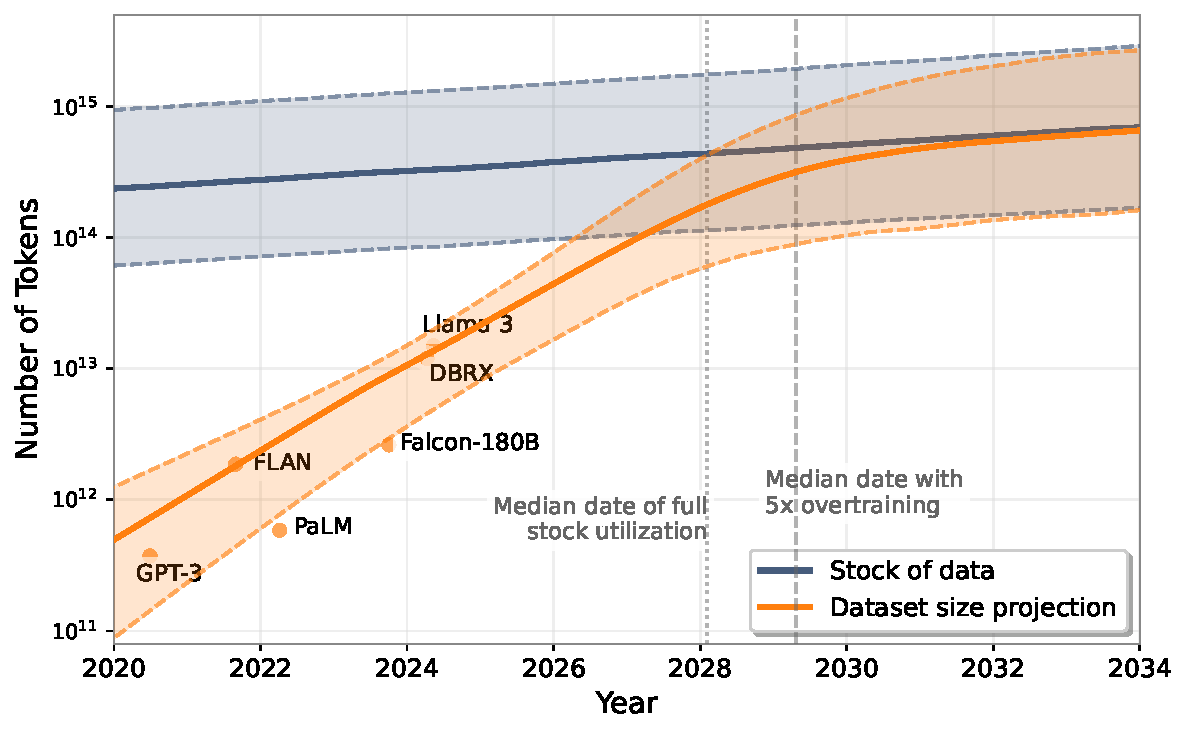
\includegraphics[width=\linewidth]{figs/projections.pdf}
%     \caption{Comparison between the projected growth of available public training data (\textcolor[RGB]{70,92,124}{blue}) and model dataset size requirements (\textcolor[RGB]{255, 127, 14}{orange}) from 2020 to 2034. The available stock of public training data will be fully utilized by around 2028.}
%     \label{fig:proj}
% \end{figure}

% 数据的需求很高
% \textbf{The Imminence of Data Exhaustion.} 
% With the rapid development of LLMs, the demand for data is growing exponentially. According to neural scaling laws, the improvement in model performance relies on the increase in the scale of training data \cite{hoffmann2022training}. 
% % Taking GPT-3 as an example, its training dataset size has reached hundreds of billions of tokens, encompassing diverse data types such as books, web pages, and code \cite{brown2020language}. 
% Taking GPT-3 as an example, its training dataset size has reached 300 billion tokens, encompassing diverse data types such as books, web pages, and code \cite{brown2020language}. 
% Research indicates that the size of training datasets is growing at a rate of approximately 0.38 orders of magnitude (about 2.4 times) per year \cite{villalobos2022trends}. 
% If this trend continues, models will require significantly more data in the coming years to sustain performance improvements.




% % 数据的供给赶不上需求
% However, despite the vast scale of publicly available human-generated text data on the internet, its total quantity is finite. 
% Estimates suggest that the current stock of publicly available human-generated text data is around 4e14 tokens (approximately 400 trillion tokens) \cite{villalobos2022trends}. 
% As shown in Figure~\ref{fig:proj}, if the current trends in LLM development persist, models are expected to exhaust the entire stock of publicly available human-generated text data by around 2028 \cite{villalobos2024will}. 
% If models are overtrained, this timeline could be accelerated to as early as 2026 \cite{villalobos2024will}. 
% Overtraining refers to the practice of using more data than what is compute-optimal during model training. While this can improve inference efficiency, it accelerates the consumption of data.
% Data exhaustion will lead to a stagnation in model performance improvements unless new data sources are found or data efficiency is enhanced.
% % The expansion of computational resources is also constrained by factors such as energy efficiency and chip production capacity \cite{ho2023limits}. 
% Therefore, the finite nature of publicly available human-generated text data is expected to become a major bottleneck for LLM scaling within the next decade. Despite the current large scale of public data, the risk of data exhaustion is rapidly approaching as data demand continues to grow \cite{sevilla2022compute}.



% % \textbf{Potential and Challenges of Synthetic Data.}
% Faced with the threat of data exhaustion, researchers have proposed various solutions, among which synthetic data generation is considered one of the most promising approaches. By using foundation models to generate data themselves, it is theoretically possible to infinitely expand the scale of training data. For example, OpenAI generates 100 billion words of text data daily, approaching the total volume of high-quality text in the Common Crawl dataset \cite{griffin2024chatgpt}. The advantages of synthetic data lie in its scalability and low cost, especially in specific domains such as mathematics, programming, and games, where synthetic data has already demonstrated significant effectiveness \cite{yang2023leandojo, liu2023tinygsm}.

% However, the use of synthetic data also faces numerous challenges. 
% First, model collapse is a serious issue. When models repeatedly train on their own generated data, they may gradually deviate from the original data distribution, leading to increasingly homogeneous and less diverse outputs \cite{shumailov2023curse}. 
% Research shows that iterative training on synthetic data can result in performance degradation and even negative returns \cite{singh2023beyond}. 
% Second, the quality of synthetic data is difficult to guarantee. While in certain domains (such as mathematical proofs), the effectiveness of synthetic data can be ensured through verification mechanisms, in complex tasks like natural language processing, the quality of synthetic data is often hard to evaluate \cite{alemohammad2023self}.
% Additionally, the diversity of synthetic data is a critical issue. To ensure that models can learn a broad range of knowledge, synthetic data needs to cover diverse linguistic styles, topics, and cultural contexts. However, existing synthetic data generation methods often struggle to produce sufficiently diverse data, limiting their application in general-purpose language models \cite{fan2023scaling}. Therefore, although synthetic data has shown promise in specific tasks, its widespread application in general language models requires further research and technological breakthroughs.



\paragraph{Public data for pretraining is exhausting.} The rapid advancement of large language models has created an insatiable appetite for training data. Neural scaling laws establish that model performance improves predictably with data quantity—a relationship that demands exponentially growing datasets \cite{hoffmann2022training}. A canonical example is GPT-3, trained on {300 billion tokens} spanning books, web content, and programming code \cite{brown2020language}. Current projections suggest dataset sizes grow at 0.38 orders of magnitude (2.4$\times$) annually \cite{villalobos2022trends}, implying models will require {three orders of magnitude more data} within a decade.

Despite the internet's vast textual resources, the total stock of high-quality human-generated text remains bounded. Recent estimates place this limit at approximately {$4\times 10^{14}$ tokens} \cite{villalobos2022trends}. \citet{villalobos2024will} argues that current consumption patterns suggest exhaustion of public text data by 2028, potentially accelerated to 2026 through excessive data reuse during training (a practice termed {overtraining}). 
% This creates a fundamental tension: while additional data currently drives progress, unrestrained consumption threatens future advancement.
Therefore, the finite nature of publicly available human-generated text data is expected to become a major bottleneck for LLM scaling within the next decade. Despite the current large scale of public data, the risk of data exhaustion is rapidly approaching as data demand continues to grow \cite{sevilla2022compute}.

% Synthetic data generation presents a paradoxical opportunity. 
\paragraph{Synthetic data has potential but faces challenges.}
Faced with the threat of data exhaustion, researchers have proposed various solutions, among which synthetic data generation is considered one of the most promising approaches. 
By leveraging LLMs to produce their own training data, researchers envision {self-sustaining data ecosystems}. Early successes in constrained domains like mathematics and code generation, where automated verification ensures quality, demonstrate potential \cite{liu2023tinygsm}.  Recent work \cite{chen2024diversity} demonstrated that diverse synthetic data enhances the performance of LLMs during both pre-training and fine-tuning.

% Industrial implementations already achieve remarkable scale—OpenAI reportedly generates {100 billion synthetic tokens daily}, rivaling major web-crawled corpora \cite{griffin2024chatgpt}.

The adoption of synthetic data faces three fundamental challenges. First, \textit{model collapse} occurs when models iteratively train on their own outputs, causing gradual divergence from original data distributions. This recursive process amplifies biases and reduces output diversity, ultimately degrading model performance across generations \cite{shumailov2023curse,dohmatob2024strong}. 
Second, \textit{synthetic data quality} remains inherently unverifiable in open-domain contexts. While formal domains like mathematics allow algorithmic validation, natural language lacks objective evaluation standards. The absence of ground-truth verification creates self-referential quality assessments, compromising reliability \cite{alemohammad2023self,wenger2024ai}.
Finally, synthetic data struggles to replicate human \textit{linguistic diversity}. Current methods disproportionately replicate dominant language patterns while underrepresenting cultural nuances and low-frequency expressions. This homogeneity limits their utility for training robust general-purpose models \cite{fan2023scaling}.

These persistent challenges underscore that synthetic data alone cannot sustainably address the looming data scarcity crisis, compelling the research community to seek complementary strategies that transcend conventional data acquisition paradigms.





% 3.3 算力垄断与成本高企
% \subsection{Computing Power Monopoly and High Costs}\label{subsec:compute_monopoly}
\subsection{The Monopoly of Computing Resources}\label{subsec:compute_monopoly}
\paragraph{A few AI giants dominate the computing power.}
The AI computing landscape is dominated by a few major tech giants like OpenAI, Google, Microsoft, and Meta, which control powerful hardware such as GPUs and TPUs. This monopolization creates a significant barrier for smaller AI startups and research institutions, who struggle to access such advanced resources. Additionally, these companies control proprietary AI models, datasets, and software frameworks that require immense computing power, further widening the gap between the giants and smaller players. As a result, high-performance computing resources remain increasingly inaccessible to anyone outside these dominant entities.

\begin{figure}
    \centering
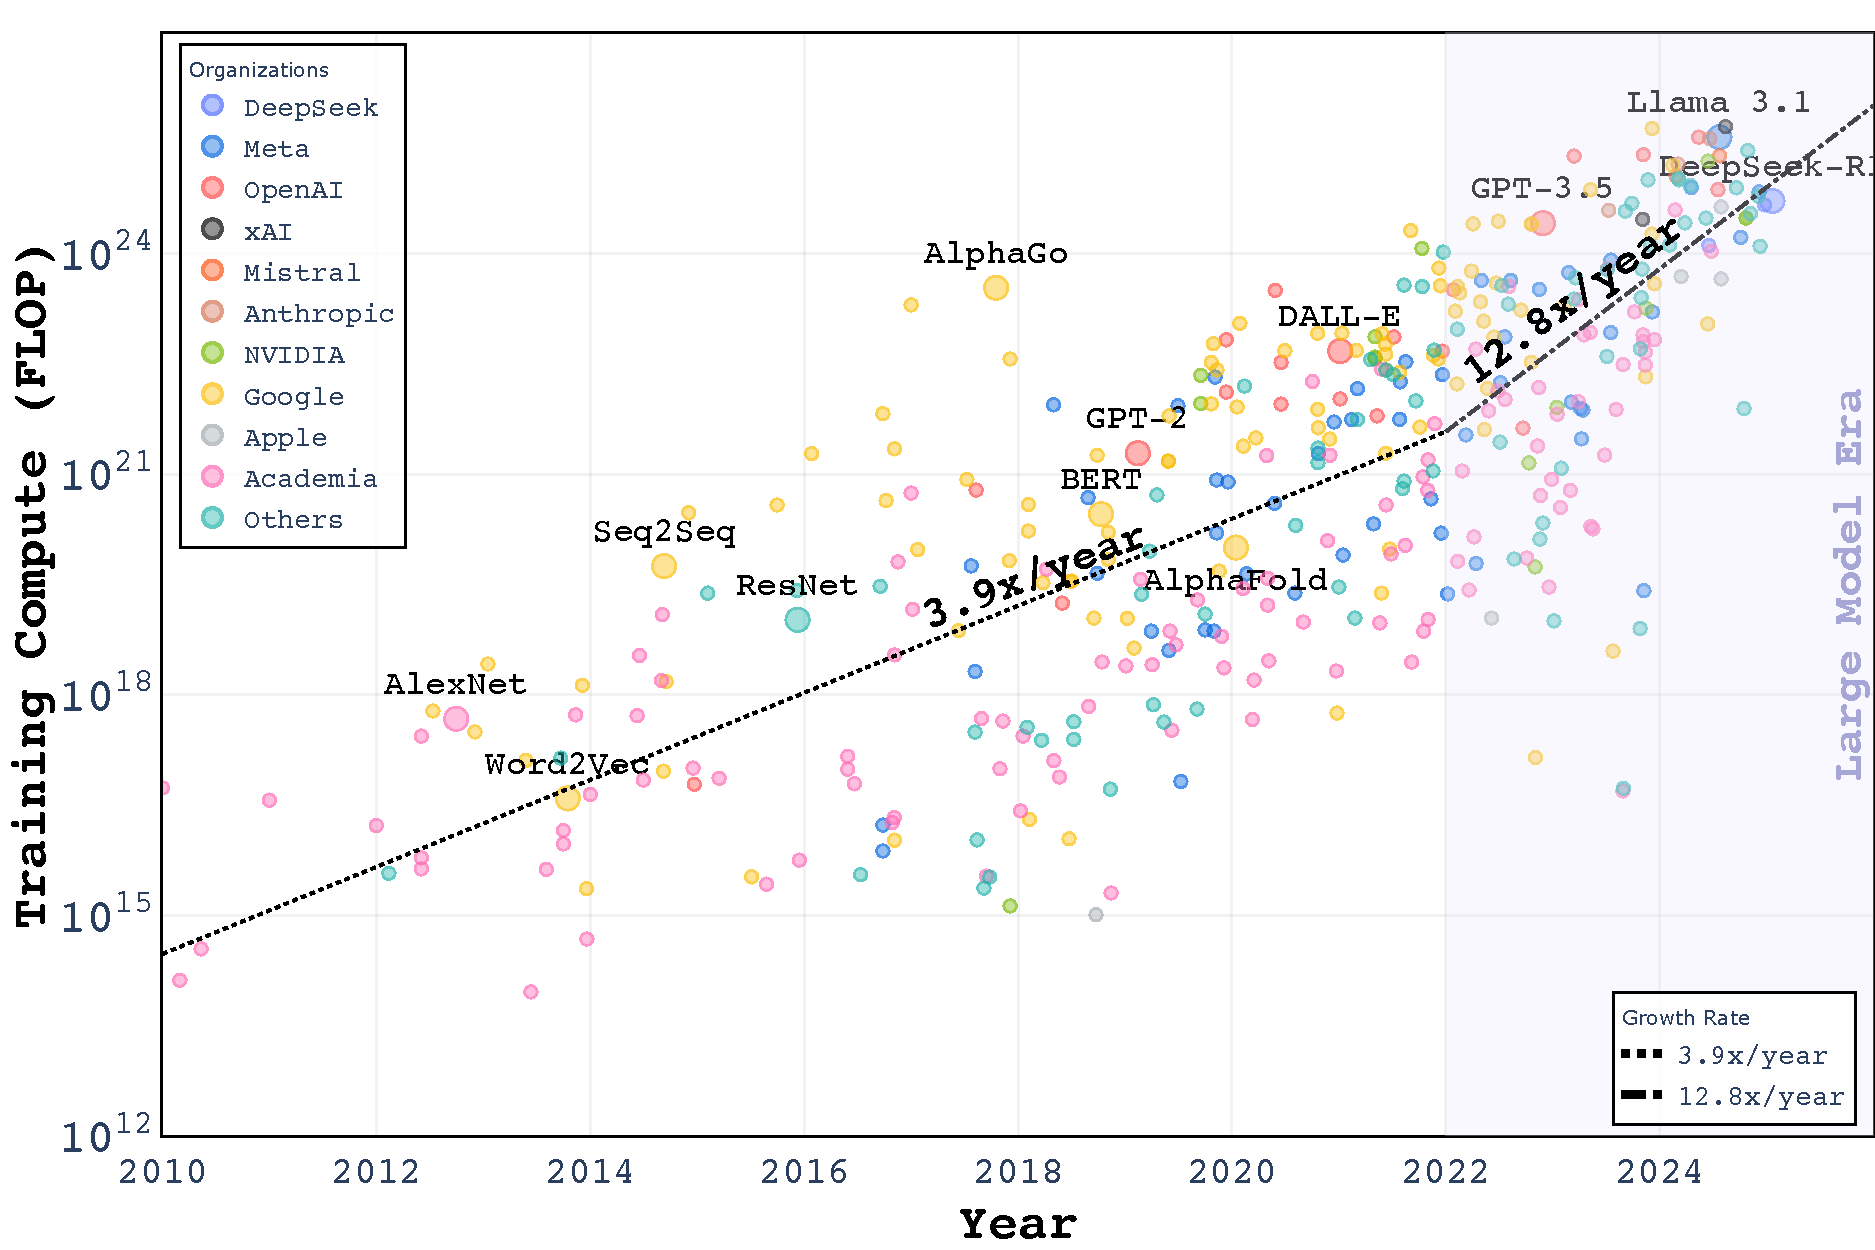
\includegraphics[width=\linewidth]{./figs/ai_compute_trend.pdf}
\vspace{-20pt}
    \caption{Trend of Computational Demand for Model Training. (Data source: Notable AI models~\cite{epoch2023trendsinmachinelearninghardware}).}
    \label{fig:model_comput_trend}
\end{figure}


\paragraph{Computational demand is growing exponentially.}
As large-scale AI models like GPT-4~\cite{openai2023gpt4}, Llama 3~\cite{meta2024llama3.1}, and DeepSeek-V3~\cite{liu2024deepseek} surpass the trillion-parameter scale, the global AI landscape faces severe computational efficiency challenges. As shown in Figure~\ref{fig:model_comput_trend}, since the deep learning revolution in 2010, AI training demands have grown at a super-exponential rate of 3.9$\times$ per year—an acceleration that intensified with the adoption of the transformer architecture as the industry standard \cite{vaswani2017attention}. With the advent of the era of large language models in 2022, the demand for computing power has surged even further, reaching an unprecedented growth rate of 13.4$\times$ per year. This marks a transformative shift in AI computation, where the need for computing power is expanding at an unprecedented pace, pushing the limits of existing hardware and infrastructure.

% Take Meta's Llama 3 as an example: its 405 billion parameters require a computing cluster of 24,000 NVIDIA H100 GPUs, consuming 30.8 million GPU hours—the equivalent of a single GPU running non-stop for 3,516 years. The hardware alone costs \$720 million while factoring in power, cooling, and operational expenses pushes total training costs beyond \$900 million. This surge in computational demand has created a triple-layered technical bottleneck. The first challenge lies in the \textbf{rapid expansion of model sizes}. The "New Moore's Law" projects a 40× increase in model parameters every 18 months, dramatically extending training cycles from weeks to months \cite{fan2023scaling}. The second challenge stems from the \textbf{escalating complexity of parallel computing architectures}. Ensuring training efficiency now requires exponentially more intricate hybrid strategies for data and model parallelism, demanding hundreds of engineer-months for optimization. Finally, the \textbf{hardware constraints} are increasingly prohibitive, with high-precision training presenting significant challenges in terms of memory bandwidth and interconnect requirements, pushing the limits of existing computing infrastructure.



\paragraph{Moore's Law is slowing down.}
Moore's Law, which has driven the growth in computing power for decades, is slowing down as we approach the physical limits of silicon-based chip technology~\cite{kressel2023end}. The difficulty in shrinking transistors has led to diminishing returns in computational performance. As a result, the AI industry is relying more on specialized hardware like GPUs, TPUs, and custom chips to meet growing demands. However, this shift has made high-performance hardware even more expensive and exclusive, further intensifying the gap between organizations with the resources to develop advanced AI models and those without.

\paragraph{Infrastructure capacity is a constraint.}
% The rapid growth in AI model size and computational demand has exposed significant capacity constraints in global computing infrastructure. Despite advances in specialized hardware, the resources required to train state-of-the-art models are outpacing existing data center capacities, leading to logistical challenges in scaling up production. Additionally, the immense energy consumption needed for these computations raises environmental concerns, contributing to a growing carbon footprint. Until more energy-efficient hardware and sustainable practices are developed, these cost and environmental issues will remain key challenges.
The rapid expansion of AI model scales and the surge in computational demand are facing dual constraints in global computing infrastructure. On one hand, bottlenecks in advanced semiconductor manufacturing severely limit the expansion rate of AI data centers. The foundry capacity for wafers at 5nm and below—such as those produced by TSMC—has already been fully booked by leading technology companies until 2026~\cite{benzinga2024tsmc}. Moreover, the construction of new wafer fabs involves long lead times and is further constrained by the global supply chain shortages of critical equipment, such as lithography machines.
On the other hand, the exponential increase in chip deployment within individual AI clusters is putting immense pressure on the already limited semiconductor manufacturing capacity, pushing the industry toward its production ceiling~\cite{scaleflux2024ai}.
These factors have significantly hindered the continuous expansion of computing power, making it increasingly difficult to scale AI infrastructure sustainably.

% - 当前算力资源的分布情况如何?(极少数AI巨头垄断了绝大部分算力资源)
% - 大规模算力需求是如何增加的?(从BERT到GPT-4算力曲线的指数级增长,模型扩展带来的成本上涨)
% - 摩尔定律放缓。
% - 产能

% % 3.4 解决方向概述
% \subsection{Overview of Potential Solutions}
% % - 针对上述挑战,有哪些方向可以探索?(例如,更高效的数据利用方式、更具普惠性的算力分布)
% % - 对于Scaling Law失效、数据枯竭和算力瓶颈,联邦学习和边缘设备是否有潜力成为解决方案?
% 逻辑主线: 终端设备隐藏的巨大数据与算力潜力如何解决当前数据枯竭和算力集中问题?

% 第4章:海量终端设备带来的AI新机遇
% \section{Opportunities and Benefits}
\section{Scaling Beyond Limits: Opportunities from Edge Devices}
\label{sec:opportunities}
% \section{New Opportunities through Edge Devices}
% The Hidden Potential from Edge Devices.  
% - 统计终端设备量。
% - 统计终端设备量。
% 4.1 海量终端数据: 冰山下的巨大能量
\subsection{Massive Data from Edges}
\label{subsec:edge_data}
% - 公共数据只占全量数据的冰山一角
% - 单个设备数据存储量很大
% - 全球活跃终端设备的规模有多大?(数十亿设备是否足够弥补当前公共数据枯竭)
% xxxxxx- 哪些类型的数据可以从终端设备中挖掘?(对话,纯文本等)输入法
% - 本地化数据的质量相比公共数据如何?
% \begin{figure}
%     \centering
% 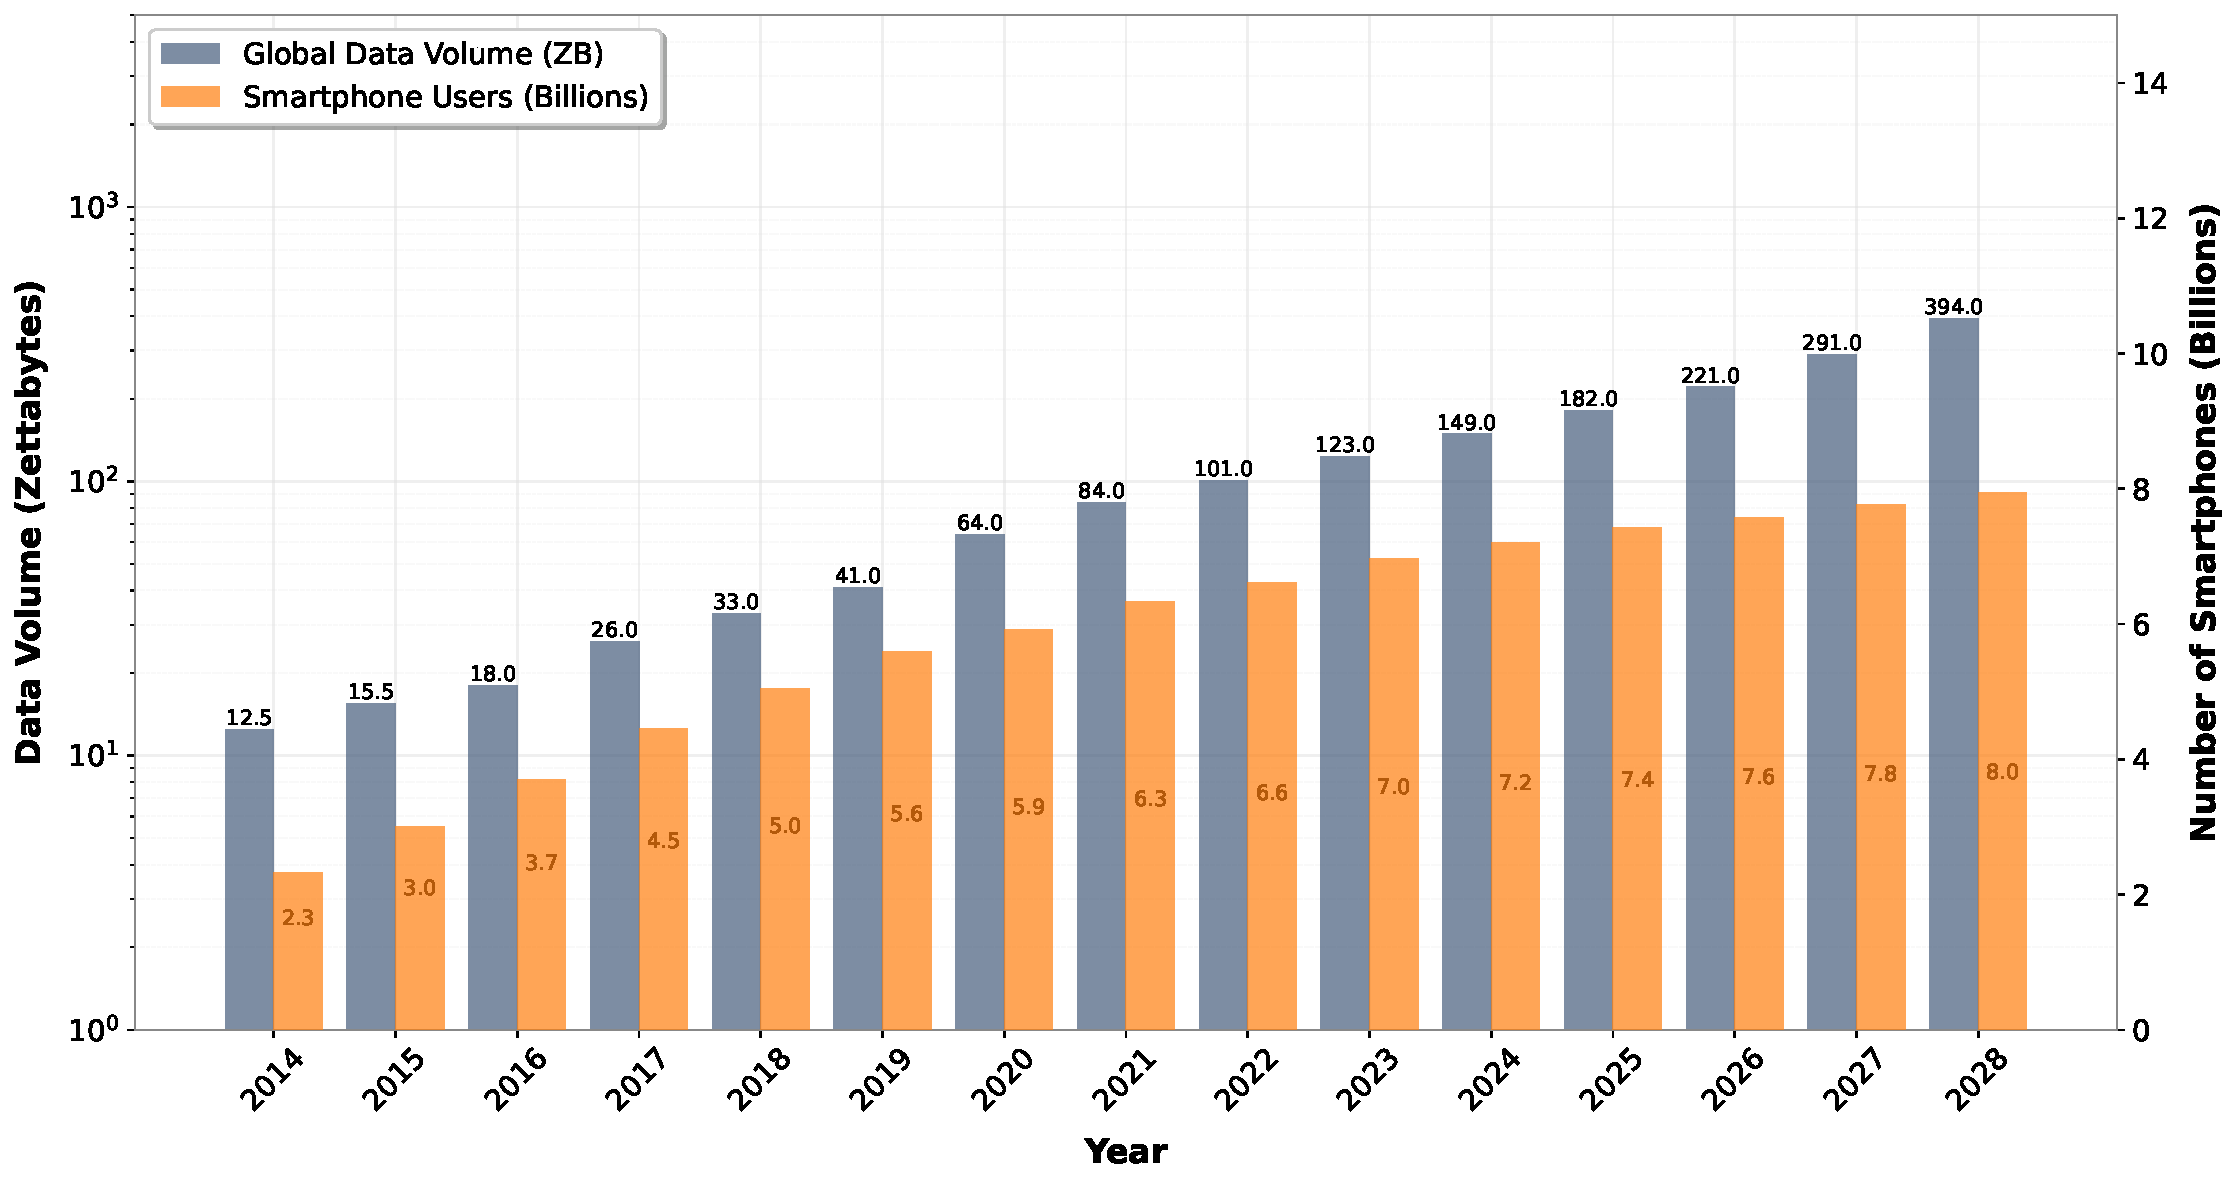
\includegraphics[width=\linewidth]{./figs/trends_bar.pdf}
%     \caption{Global Data Volume and Smartphone Users Growth from 2014 to 2028.}
%     \label{fig:proj}
% \end{figure}

% \begin{figure}
%     \centering
% 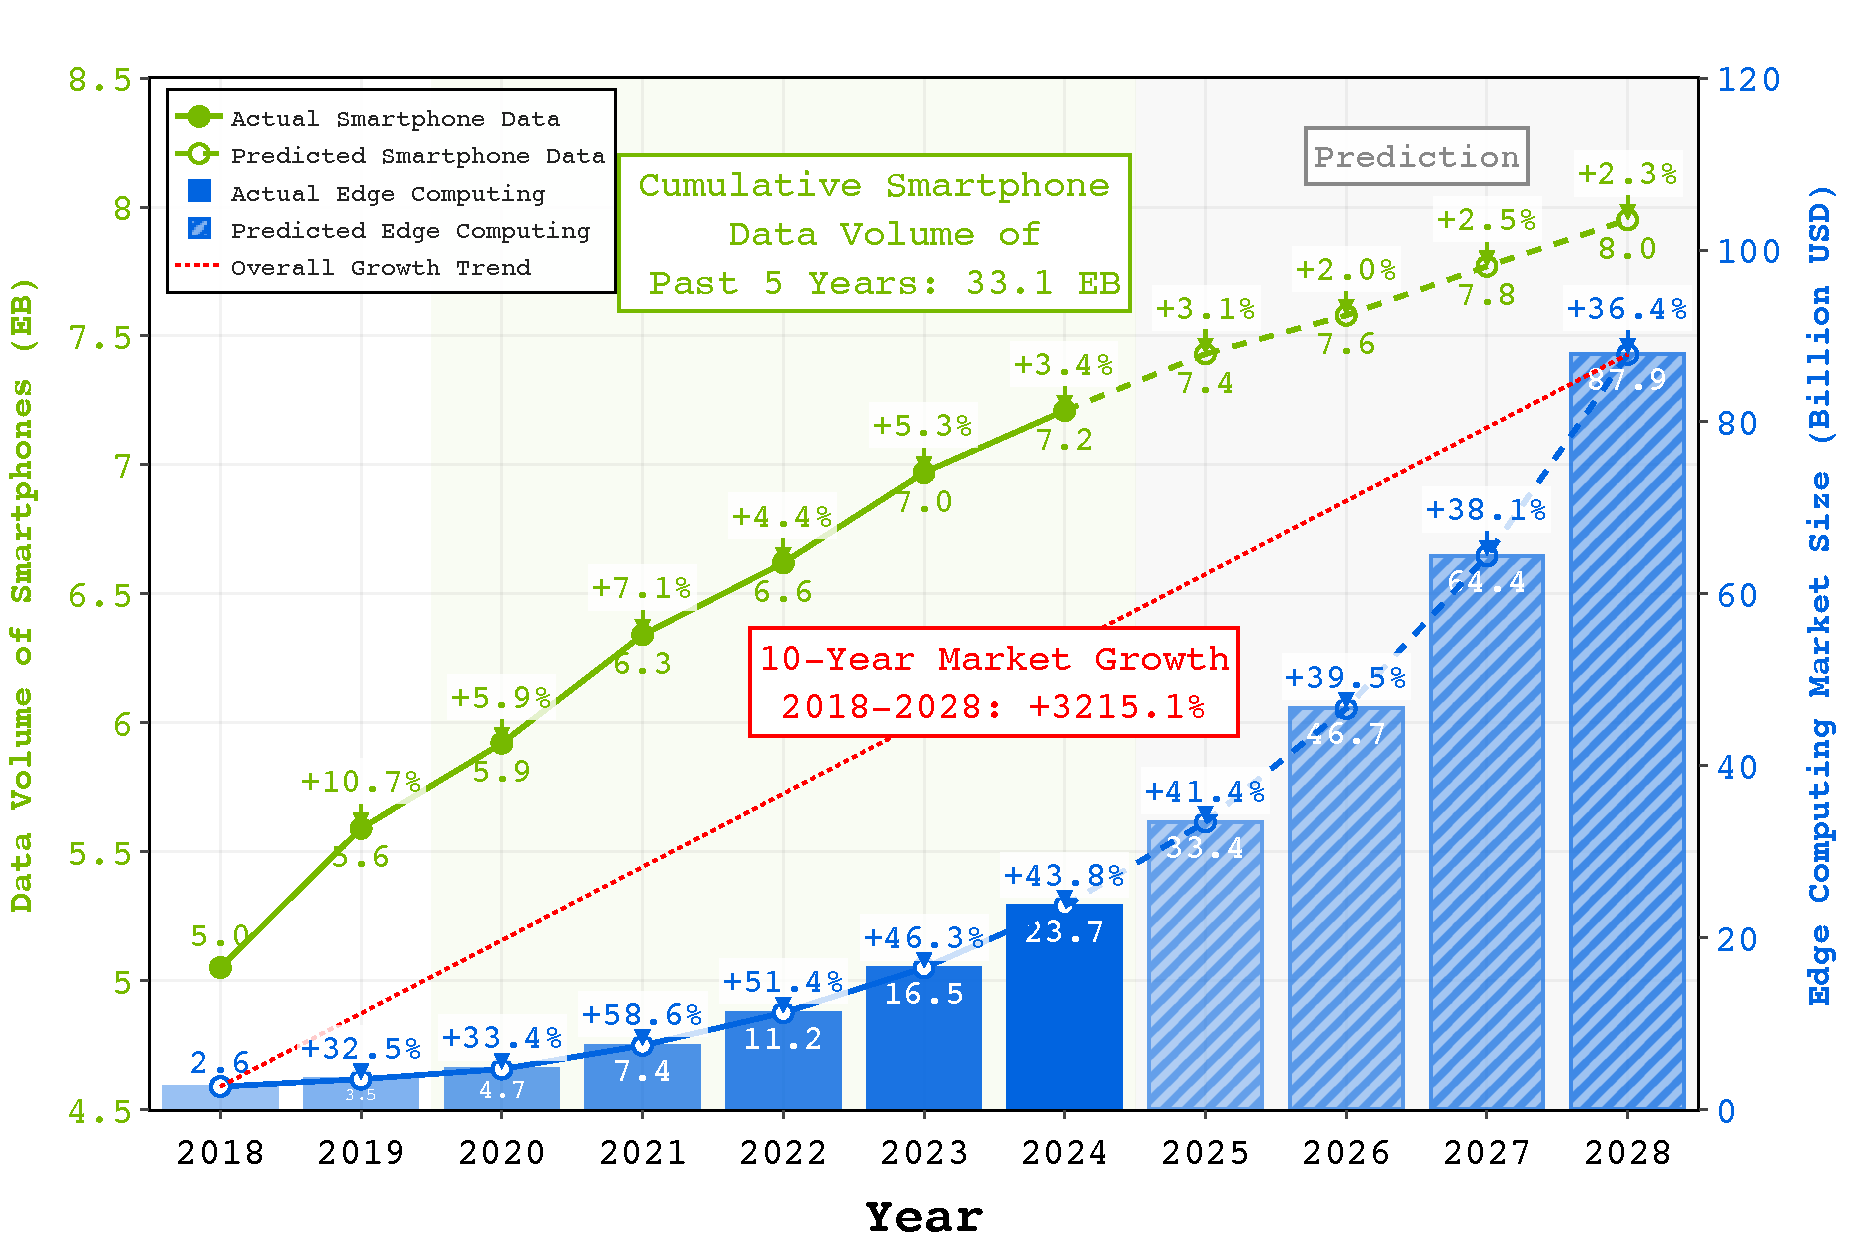
\includegraphics[width=\linewidth]{./figs/edge_and_smartphone.pdf}
%     \caption{Smartphone users growth with edge computing market size (right) from 2014 to 2028.}
%     \label{fig:proj}
% \end{figure}

\begin{figure*}[htbp]
    \centering
    \begin{minipage}[t]{0.49\linewidth}
        \centering
        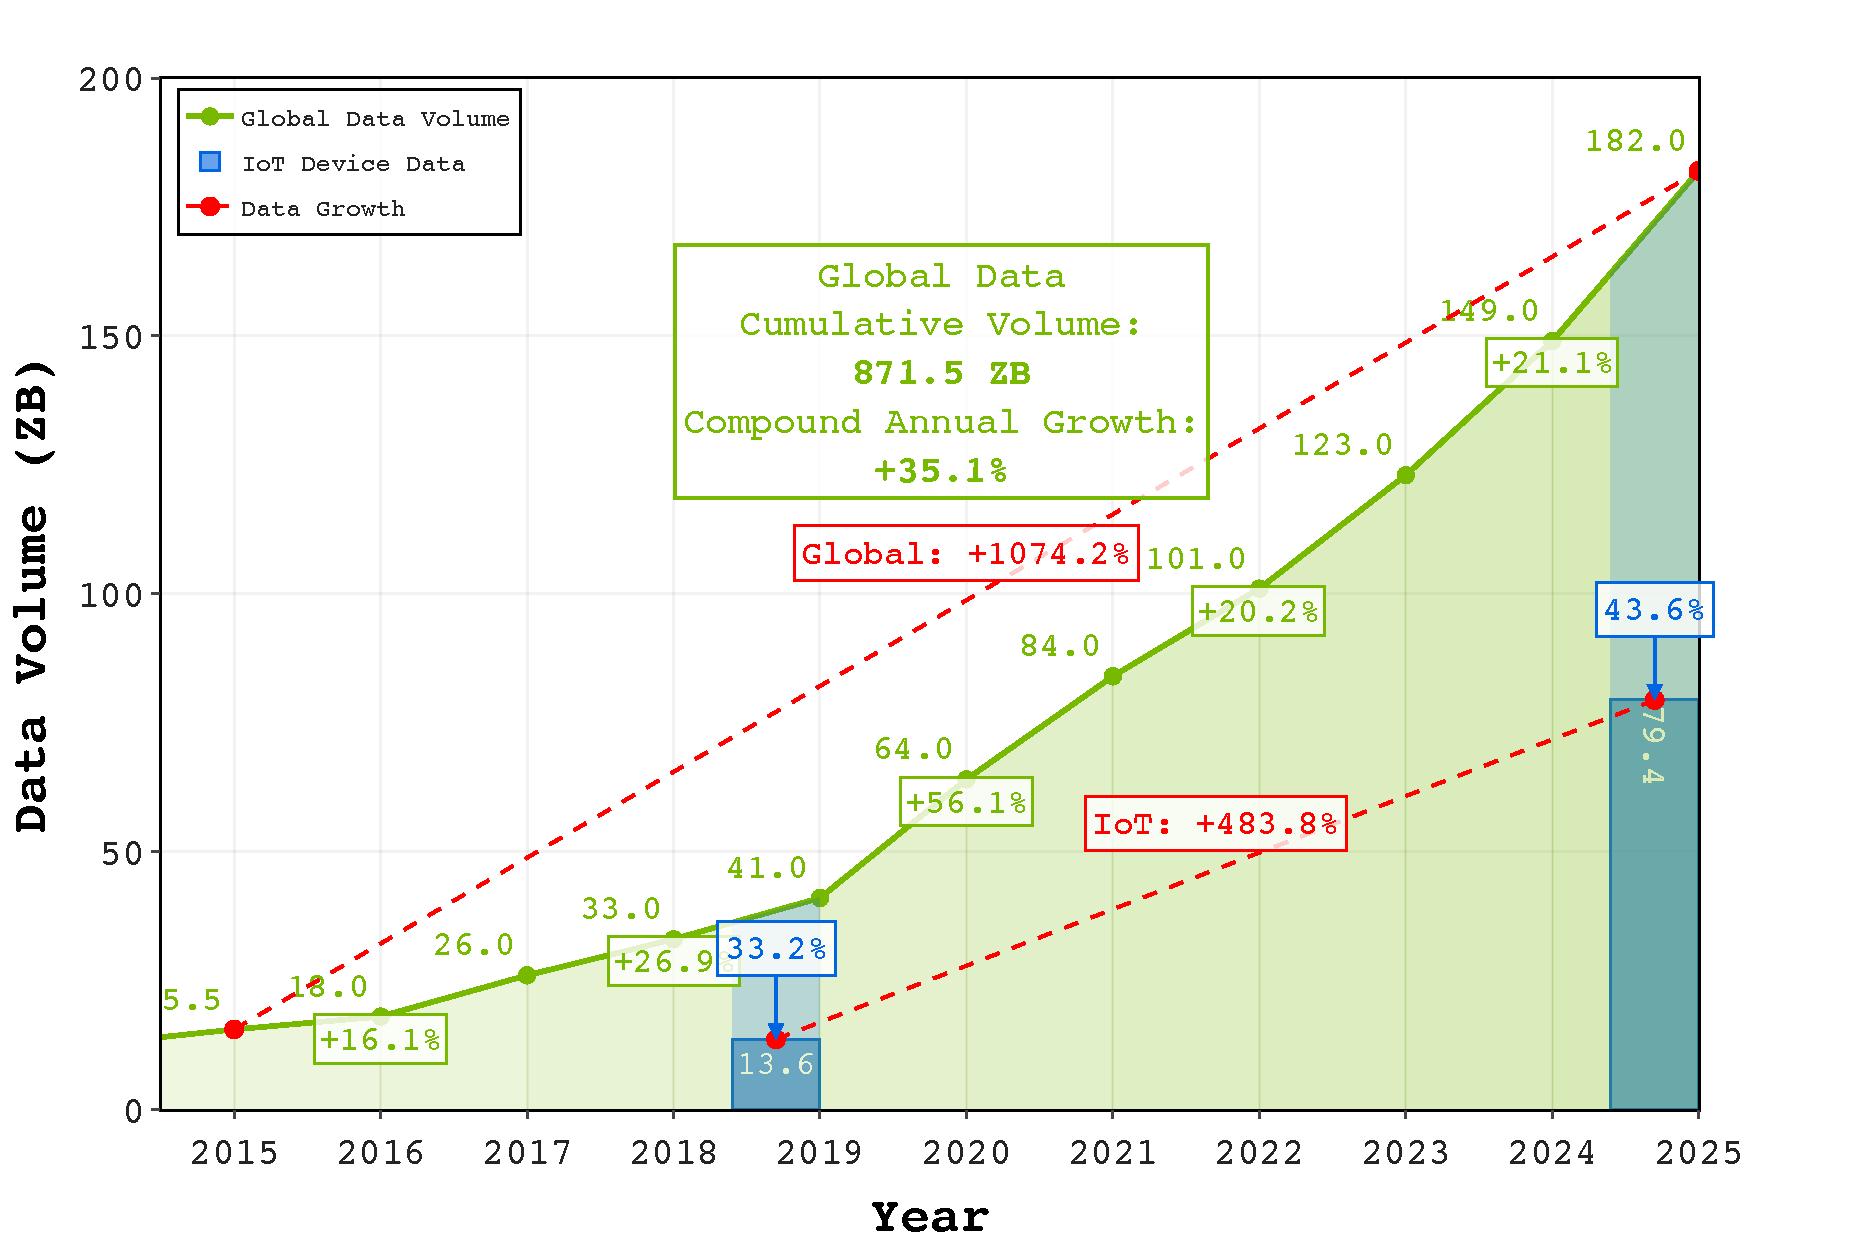
\includegraphics[width=\linewidth]{./figs/iot_data_contribution.pdf}
\vspace{-20pt}
        \caption{Global data volume from 2014 to 2025 and IoT device data volume in 2015 and 2025. (Data sources: Global data volume from \cite{statista_global_2023}; IoT device data volume from \cite{statista_iot_2023}.)}
    \label{fig:global_data}
    \end{minipage}
    \hfill
    \begin{minipage}[t]{0.49\linewidth}
        \centering
        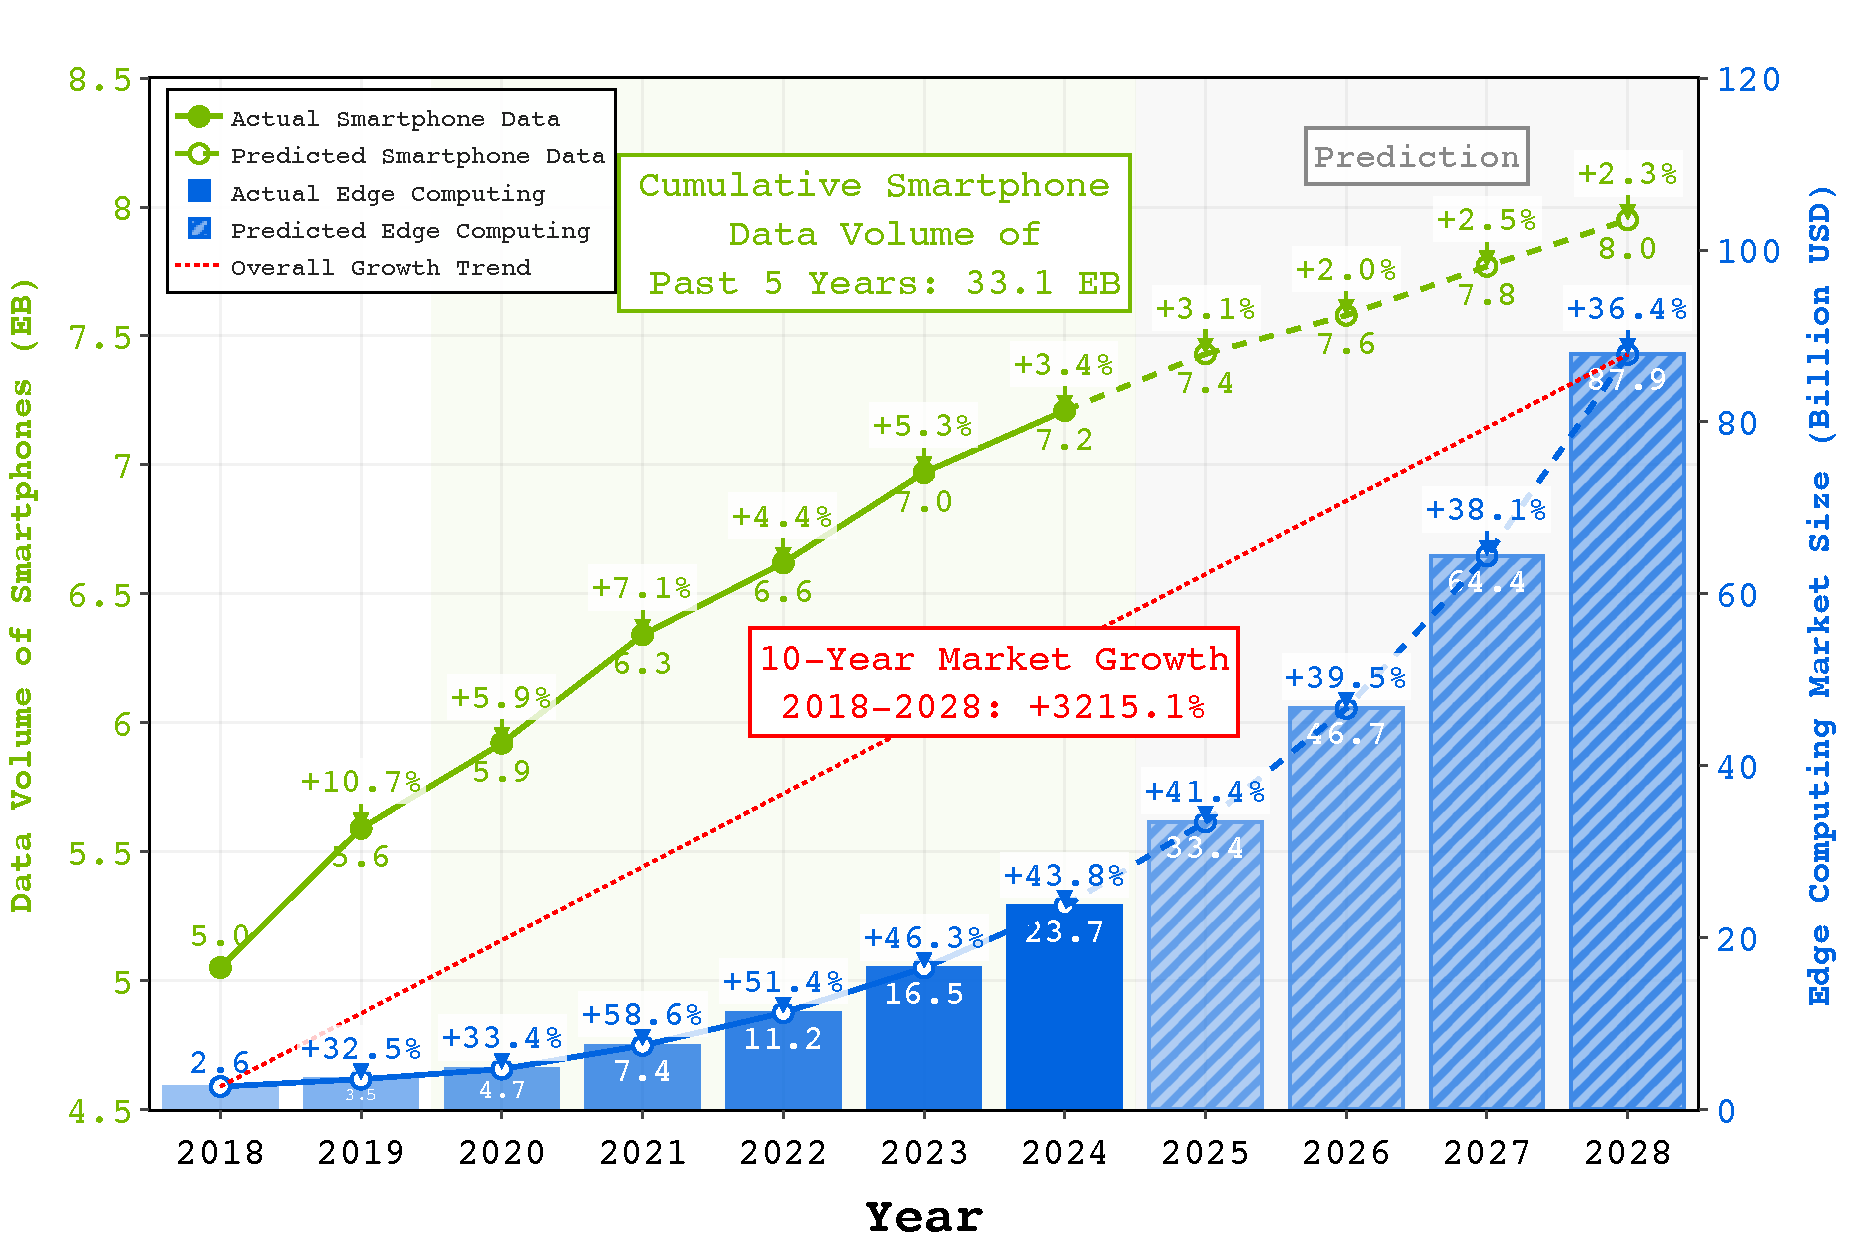
\includegraphics[width=\linewidth]{./figs/edge_and_smartphone.pdf}
\vspace{-20pt}

        \caption{Smartphone data volume with edge computing market size (right) from 2018 to 2028. (Data sources: Edge computing market \cite{grandview_edge_2023}; Smartphone data volume derived from the number of smartphones \cite{bankmycell_smartphone_2023}.)}
    \label{fig:smartphone}
    \end{minipage}
    
\end{figure*}


% As mentioned in \S\ref{subsec:data_exhaustion}, in addition to synthetic data, edge data is considered another important avenue for addressing the issue of data exhaustion. 
% While publicly available data is vast, it represents only the tip of the iceberg in terms of total data volume. In contrast, the amount of data generated by edge devices (such as smartphones, tablets, and IoT devices) is significantly larger and exhibits high diversity and personalization. 
% According to estimates in the literature, the number of active edge devices worldwide has reached billions, with each device generating several to tens of gigabytes of data daily~\cite{villalobos2022trends}. This data encompasses various types, including user conversations, input method records, and sensor data, offering immense potential value.

% The types of data generated by edge devices are highly diverse, primarily including user conversation data, input method data, and sensor data. Instant messaging applications (such as WhatsApp and WeChat) generate hundreds of billions of messages daily, with each message containing an average of 4-5 tokens~\cite{rosenfeld2018whatsapp}. 
% These data not only include textual information but may also encompass multimedia content such as voice, images, and videos. Smartphone input methods record users' typing habits, frequently used vocabulary, and language styles, which can help models better understand the diversity and complexity of natural language. Additionally, sensor data (such as location, temperature, and motion data) generated by IoT devices (e.g., smart home devices and wearables) can provide additional contextual information for models, particularly in multimodal tasks.

% Compared to public data, local data has significant advantages in terms of quantity and quality. First, in terms of quantity, the scale of local data far exceeds that of public data. Taking social media platforms as an example, Facebook generates approximately 10 trillion tokens of text data annually, while Twitter and Instagram generate around 1.5 trillion and 800 billion tokens, respectively~\cite{villalobos2022trends}. This data is not only massive in scale but also highly diverse and real-time, making it a valuable resource for training language models. In contrast, public datasets (such as Common Crawl) have a total volume of about 400 trillion tokens, and their growth rate is relatively slow~\cite{hoffmann2022training}.

% Second, in terms of quality, local data typically exhibits higher personalization and contextual relevance. Although public data undergoes some cleaning and filtering, its content is often generic and lacks deep understanding of specific users or scenarios. In contrast, local data (such as user conversations and input method records) captures users' personalized language habits, cultural backgrounds, and real-time needs, thereby providing richer contextual information for models. For example, input method data reflects users' frequently used vocabulary and expressions, while social media data includes users' interests, emotions, and social network information. Such high-quality data can help models better adapt to diverse application scenarios, improving their generalization capabilities and user experience.

% However, the utilization of local data also faces several challenges. First, privacy concerns are a major obstacle. Data on edge devices often contains sensitive user information, and how to effectively utilize this data while protecting user privacy is an urgent issue. Second, data quality and standardization are also critical challenges. Local data is often fragmented and of inconsistent quality, making effective cleaning and standardization a technical hurdle. Finally, legal and ethical issues constrain the use of local data. Using local data for model training may pose legal risks, particularly regarding user privacy and data ownership.

% Despite these challenges, the potential of local data cannot be overlooked. Through technologies such as federated learning, it is possible to utilize data from edge devices for model training without compromising user privacy~\cite{konevcny2016federated}. Moreover, social media companies (such as Meta and Twitter) have begun exploring the possibility of using their own data for model training. For example, Meta's Llama series of models partially leverages user-generated content from Facebook and Instagram for training~\cite{touvron2023llama}. This "self-sustaining" model not only alleviates the issue of data exhaustion but also enhances the personalization and localization capabilities of models.

% Therefore, the utilization of edge data and social media data holds promise as an important supplement to address the issue of data exhaustion, especially as publicly available data becomes increasingly scarce. Through technological innovation and privacy protection measures, edge data and social media data can provide a sustainable source of data for model training.

As discussed in §~\ref{subsec:data_exhaustion}, edge data represents a crucial alternative to synthetic data in addressing the challenge of data exhaustion. Edge data refers to the data generated by edge devices at or near the source of data generation, which typically remains private and localized rather than being publicly accessible. Edge devices encompass a wide range of equipment including Internet of Things (IoT) sensors, smartphones, wearables, industrial controllers, and other smart devices that process data at the network edge. The global data ecosystem exhibits significant bifurcation: publicly available data constitutes merely the tip of the iceberg, while data generated by edge devices demonstrates superior strategic value both in terms of growth rate and high quality.

\paragraph{Edge-generated data is explosively growing.} 
% By 2025, it is projected that over 80\% of global data will be generated directly at the edge, rather than in traditional centralized data centers \cite{seagate_rethinkdata_2020}. This shift highlights a fundamental transformation in how data is created, processed, and utilized across industries.
As illustrated in Figure~\ref{fig:global_data}, the global data volume is projected to reach 182 ZB by 2025~\cite{statista_global_2023}, with a particularly pronounced growth in edge-generated data. The data generated by IoT devices is anticipated to increase from 13.6 ZB in 2019 to 79.4 ZB in 2025~\cite{statista_iot_2023}, elevating its share of the global data volume from 33.2\% to 43.6\%. Over the period from 2015 to 2025, the global data volume exhibited a compound annual growth rate (CAGR) of 35.1\%, resulting in an overall increase of 1074.2\% and a cumulative total of 871.5 ZB. IoT device data experienced a growth of 483.8\% from 2019 to 2025. This trend underscores the increasingly central role of edge-generated data in the global data ecosystem.
Beyond IoT devices, smartphones, as a critical source of edge-side data, are also contributing to the steady rise in data volume. As depicted in Figure~\ref{fig:smartphone}, the estimated smartphone data volume is projected to grow from 5 EB in 2018 to 8 EB by 2028
\footnote{These numbers are estimated based on an average user data generation of 1 GB per device. For detailed estimation methodology, refer to Appendix \ref{app:smartphone_ethod}.}. 
This exponential growth is closely aligned with the rapid expansion of the edge computing market, which is forecasted to surge from \$5.5 billion in 2019 to \$87.9 billion by 2028, representing a remarkable growth rate of 3215.1\%. The burgeoning edge computing market has further catalyzed the generation and processing of edge-side data, reinforcing its significance in the broader data landscape.
\vspace{-0.5cm}
\begin{insights}
    \textbf{Insight:} The smartphone data volume of the past 5 years (before 2025) is projected to reach approximately 33.1 EB, with unique advantages in privacy and real-time context, demonstrating the massive data potential of edge for AI model training.
\end{insights}
   
% To put this into perspective, the total volume of global data is expected to surpass 181 ZB annually by 2025 \cite{statista_global_2023}. This rapid growth is further fueled by the proliferation of IoT devices and connected technologies. As illustrated in Figure \ref{fig:global_data}, IoT devices alone are projected to account for 43.6\% of global data volume by 2025, marking a significant increase from their contribution of 33.2\% just six years prior. Meanwhile, as shown in Figure \ref{fig:smartphone}, smartphone data volume is projected to grow steadily from 3.5 EB in 2029 to 7.8 EB by 2028\footnote{Estimated using 1GB average data generation per device. See Appendix \ref{app:smartphone_ethod} for details.}, showcasing a consistent upward trajectory.
% The growth in data generation is paralleled by the expansion of the edge computing market, which is forecasted to rise from 5.5 billion in 2019 to 64.4 billion by 2028 \cite{grandview_edge_2023}, reflecting the widespread adoption of edge-centric architectures. 
% In summary, the immense volume of edge data with its rapid growth trajectory, establishes a promising foundation for pretraining at the edge.

\paragraph{Edge-generated data is of high quality.} 
Beyond its impressive quantity, edge data possesses several qualitative advantages that make it particularly valuable for model pretraining.
First, edge data exhibits superior \textit{diversity} across multiple dimensions. It encompasses a wide variety of data types from IoT devices, mobile interactions, and personal devices, covering different domains, languages, and user behaviors. This natural diversity provides richer training signals compared to curated public datasets \cite{nayak2024review}. 
Second, edge data demonstrates strong \textit{real-time capability}. Unlike public datasets, which are often updated infrequently, edge devices continuously generate fresh data with low latency \cite{cavliwireless_edgecomputing}, offering more up-to-date and relevant training samples.
Third, edge data offers enhanced \textit{personalization} characteristics. It enables real-time interactions and context-aware recommendations by leveraging local data such as location and device behavior. This allows for highly relevant and adaptive personalization that can dynamically adjust to user preferences \cite{xenonstack_edge_ai_2023}.
Fourth, edge data exhibits enhanced \textit{context awareness} due to the proximal positioning of edge devices to data sources, enabling the capture of fine-grained contextual information often absent in public datasets. For instance, wearable devices collect synchronized activity and location data, providing high-fidelity behavioral patterns that preserve temporal and spatial context.

\vspace{-0.1cm}
In conclusion, edge data with its explosive growth
\footnote{
\citet{idc_seagate_dataage_2019,seagate_rethinkdata_2020} provide a more comprehensive overview of the global data volume, but we cannot access the statistics data. 
We appreciate any suggestions for better statistical data sources.
}
and superior qualitative characteristics, is a valuable resource for model pretraining. Its diversity, real-time nature, personalization, and rich context make it an ideal foundation for developing robust and adaptable large-scale models, enhancing their ability to serve real-world applications effectively.



% Fourth, edge data provides superior \textbf{contextual completeness}, as evidenced by smart device interactions achieving 97\% contextual reasoning accuracy~\cite{llama2023}. This rich contextual information enables models to learn more comprehensive semantic relationships. 
% These characteristics - natural diversity, timely updates, diverse language patterns, and rich contextual information - make edge data an invaluable resource for enhancing the quality and effectiveness of large language model pretraining, particularly in capturing real-world language usage and user behaviors.


% \textbf{High quality of Edge-generated data.} Firstly, edge data is highly diverse. It comes from a wide variety of sources such as IoT devices, mobile phones, and wearable sensors. This diversity provides a more comprehensive and detailed view of the real-world scenarios. For example, in a smart city application, data from traffic cameras, weather stations, and air quality monitors can be combined to provide a holistic understanding of the urban environment. Secondly, edge data is more timely. Edge devices can process and analyze data in real-time or near-real-time, which is crucial for applications that require immediate responses. For instance, in an industrial automation setting, data from sensors on machinery can be used to detect faults and trigger maintenance actions before they lead to significant downtime. Thirdly, edge data is more context-aware. Edge devices are often located close to the data source, which allows them to capture context-specific information that may be lost in public data. For example, a wearable device can capture data about a user's physical activity and location, providing a more accurate picture of their behavior.

% Compared to public data, edge data demonstrates quality advantages across three dimensions: (1) \textbf{Real-time capability}: Social platform data latency typically remains under 500ms (Meta internal benchmarks), while public datasets usually update on cycles exceeding 6 months; (2) \textbf{Personalization}: The n-gram distribution in input method records shows significant user specificity, with Jensen-Shannon divergence 37\% higher than public corpora~\cite{touvron2023llama}; (3) \textbf{Contextual completeness}: Sensor data from smart home devices forms multimodal associations with user voice commands, enabling dialogue systems to achieve 97\% contextual reasoning accuracy~\cite{llama2023}. These characteristics make edge data crucial for enhancing model domain adaptability---Meta's Llama series models achieved a 12.3\% improvement in F1 score for personalization tasks by incorporating Instagram user-generated content (UGC)~\cite{touvron2023llama}.

% \textbf{Diversity of Edge-generated data.} Edge data has transcended traditional textual boundaries to form a comprehensive spectrum of multimodal sensory data: (1) \textit{Communication data}: Instant messaging applications (such as WhatsApp and WeChat) generate over 100 billion messages daily, with each message containing an average of 4-5 semantic units~\cite{rosenfeld2018whatsapp}; (2) \textit{Behavioral data}: Input method records capture user input patterns across over 200 language variants and personalized expression characteristics~\cite{tisi2023}; (3) \textit{Environmental data}: Biosensor data from smart wearables is growing at 41\% annually, with each device generating 1.2GB of physiological metrics daily~\cite{seagate2025}. This data not only vastly exceeds public datasets (Common Crawl's total volume is approximately 400 trillion tokens, with annual growth <5\%~\cite{hoffmann2022training}) but also possesses unique spatiotemporal correlations---smartphone location data combined with social media LBS information can construct user behavior profiles accurate to meter-level precision~\cite{gartner2025}.





% 4.2 海量终端算力: 云端下的巨大动力
\begin{figure*}[htbp]
    \centering
    \begin{minipage}[t]{0.49\linewidth}
        \centering
        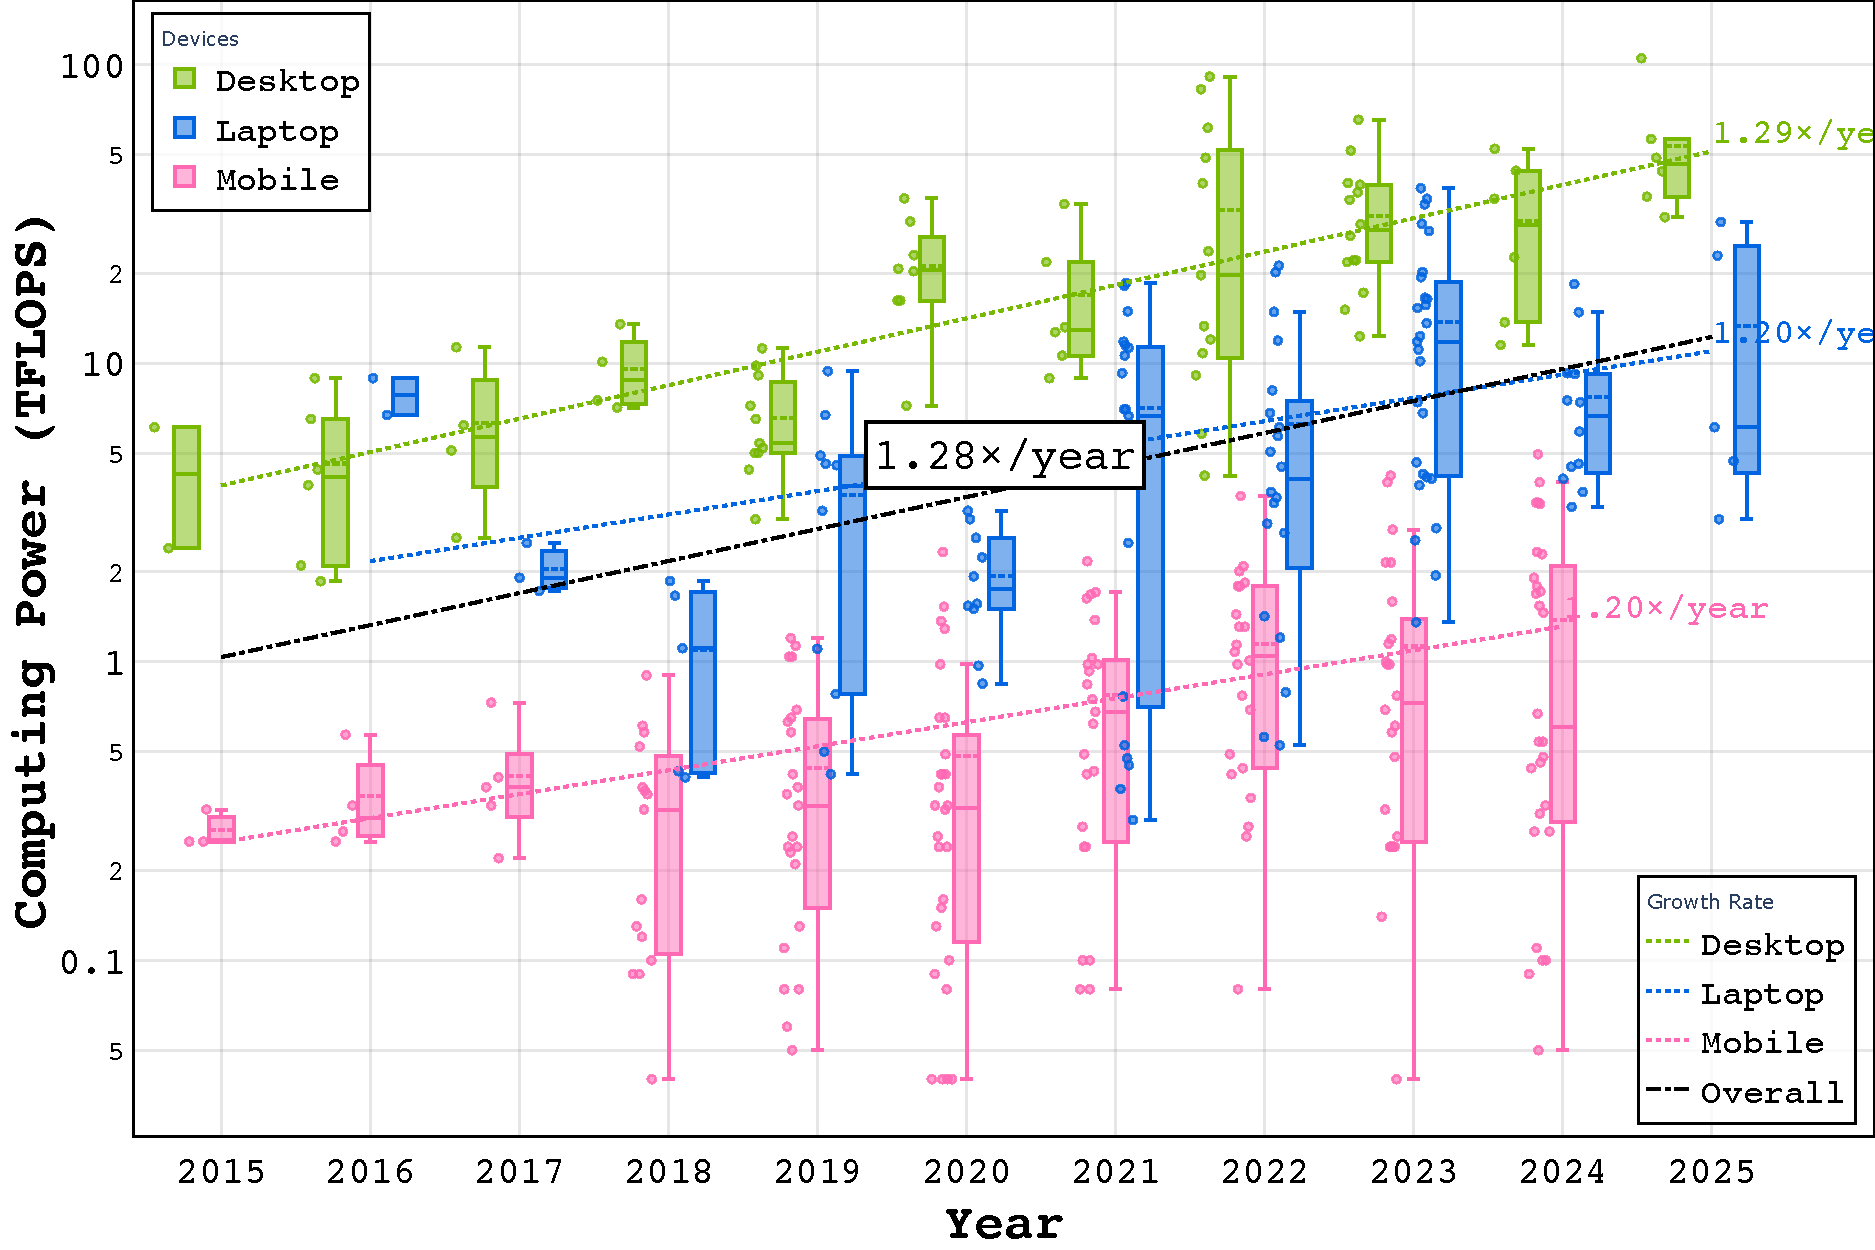
\includegraphics[width=\linewidth]{./figs/edge_compute_trend.pdf}
        \vspace{-20pt}
        \caption{Edge Computing Power Evolution Trend. (Data source: \cite{nanoreview2025}).}
        \label{fig:edge_trend}
    \end{minipage}
    \hfill
    \begin{minipage}[t]{0.49\linewidth}
        \centering
        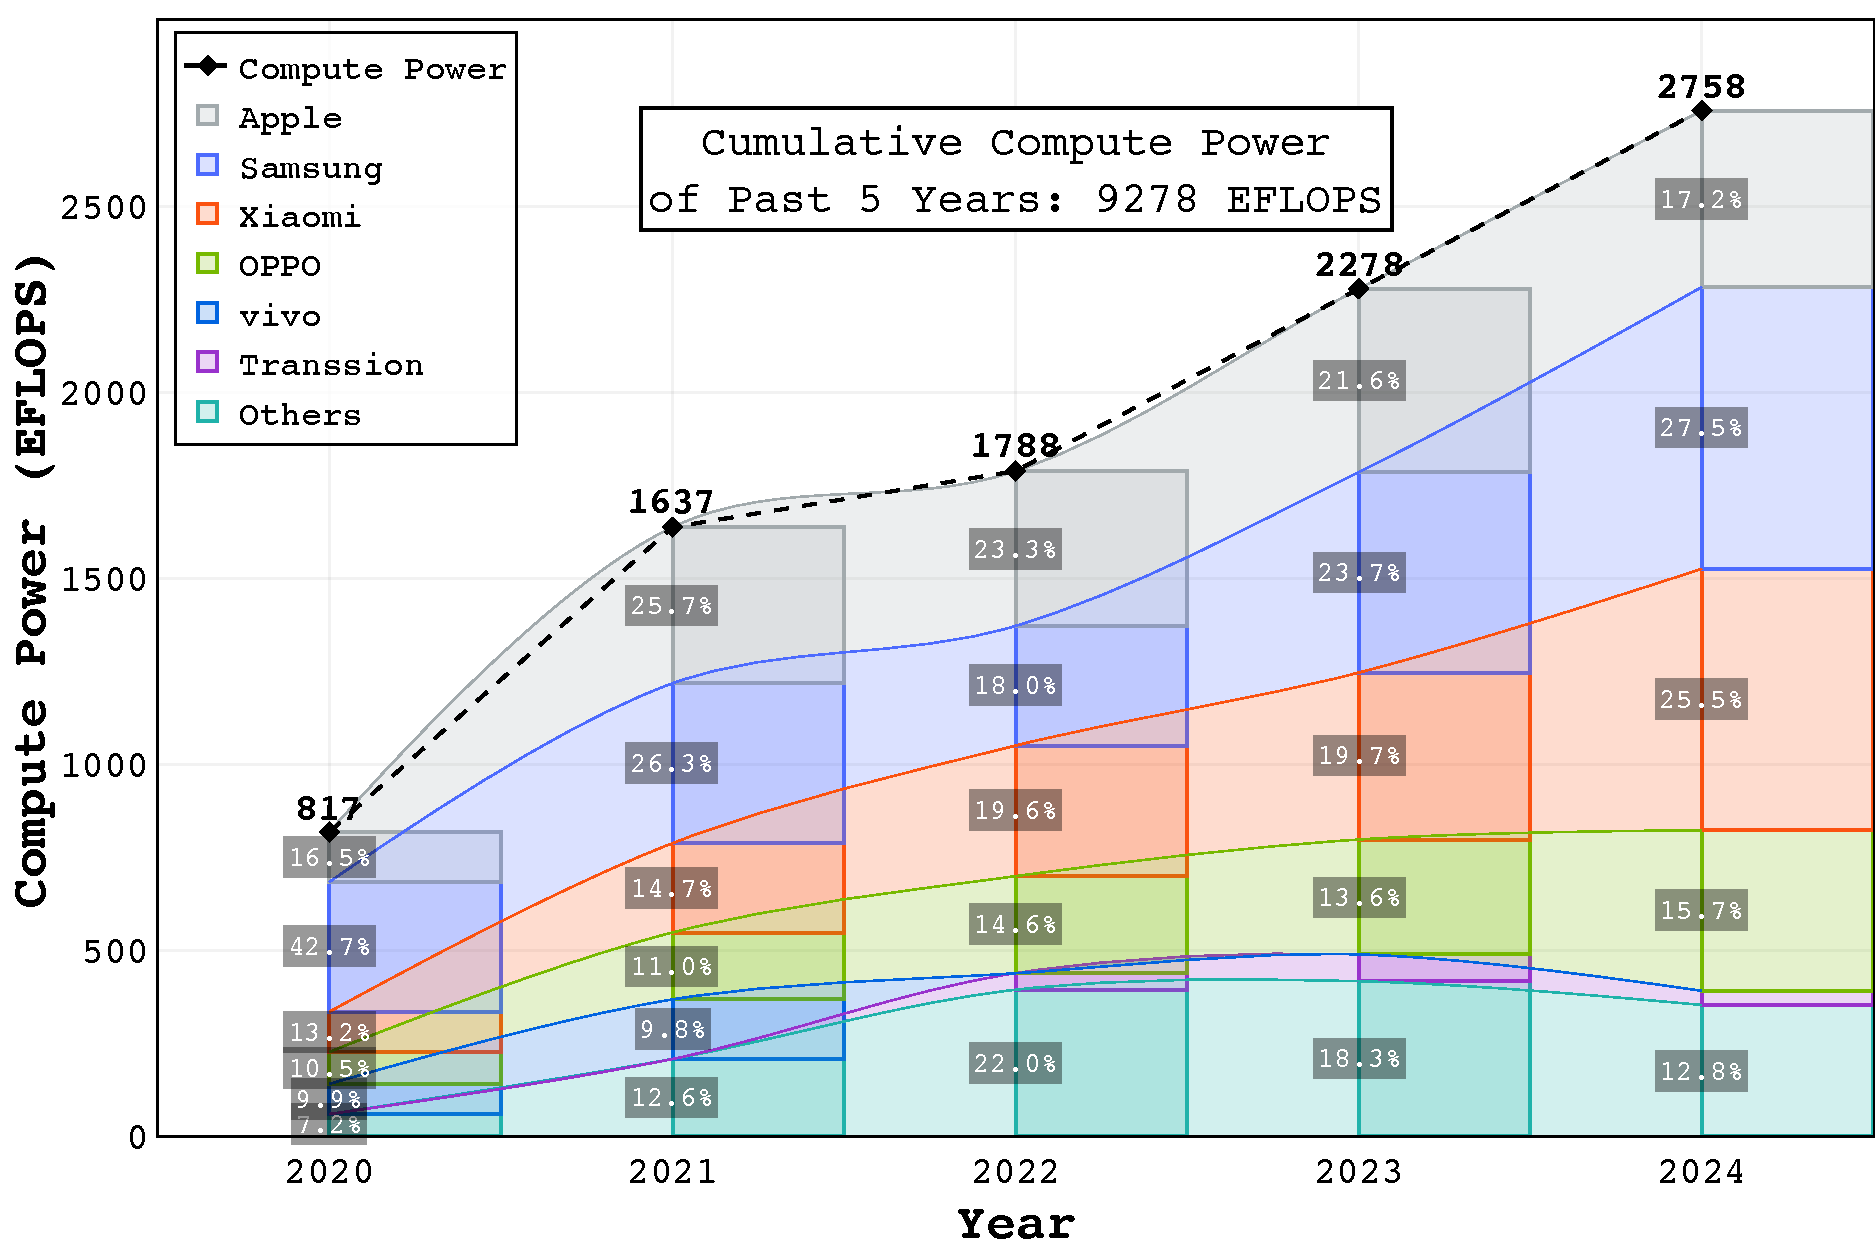
\includegraphics[width=\linewidth]{./figs/smartphone_compute_trend.pdf}
        \vspace{-20pt}
        \caption{Smartphone Market Share and Computing Power Trends. (Data source: \cite{canalys2025}).}
        \label{fig:smartphone_trend}
    \end{minipage}
\end{figure*}
\subsection{Massive Computing Power from Edges}\label{subsec:edge_compute}
% - 海量终端能提供巨大的算力
% - 单个设备(iPhone)20 TFLOPS, 单卡 200 TFLOPS,10倍。
% - Llama 算力 单卡*卡数量,TFLOPS, 得出 同等算力需要多少终端设备
% - 单个设备(iPhone)20 TFLOPS, 单卡 200 TFLOPS,10倍。
% - Llama 算力 单卡*卡数量,TFLOPS, 得出 同等算力需要多少终端设备(数字)
% - 2w 卡, 移动设备。

% 端侧算力的发展情况
% 端侧算力未来总量
% 端侧算力是否足以训练最新的模型:以Llama3和DeepSeek为例


\paragraph{Edge computing power is growing rapidly.}
In recent years, edge computing has experienced explosive growth in computing power, driving smart devices to evolve from single-function tools into multimodal perception and decision-making centers. For instance, as shown in Figure~\ref{fig:edge_trend}, flagship smartphones such as the iPhone 16 series, equipped with 3nm process chips, have achieved computing power exceeding 2 TFLOPS~\cite{apple2024iphone16pro}, enabling local execution of complex AI tasks like real-time image enhancement and multilingual speech translation. 
Notably, the computing power of an individual smartphone has potentially surpassed that of laptops in the same period.
The breakthroughs are even more pronounced in the desktop sector,
% where NVIDIA's GeForce RTX 5090, with 104.9 TFLOPS of computing power~\cite{nvidia2025}, 
achieving an annual computing power growth rate of 1.29$\times$/year, surpassing that of smartphones and laptops (both 1.20$\times$/year). 
% \footnote{{Data source: \url{https://nanoreview.net}.}}
These three types of devices form a differentiated growth hierarchy, collectively driving edge computing's overall computing power to expand at an annual average rate of 1.28$\times$/year.
% , significantly outpacing the 1.3$\times$ growth rate of cloud computing~\cite{epoch2023trendsinmachinelearninghardware}, with the gap between the two continuing to narrow. 
This growth is fueled by three key technological drivers: advanced manufacturing processes (3nm technology increases transistor density by 60\%~\cite{apple2024iphone16pro}), dedicated architectures (modern smartphone SoCs integrate NPUs for AI acceleration), and scenario-driven innovation (e.g., autonomous driving demands end-to-end latency of less than 100ms~\cite{nvidia2023}).
% The quantitative increase in computational power has led to qualitative transformations: AR/VR devices can now reduce spatial modeling latency from seconds to milliseconds~\cite{idtechex2024}; medical-grade wearable devices can perform real-time analysis of 12-lead ECG data~\cite{gopala2024}; and educational tablets are capable of rendering 8K-resolution holographic teaching environments~\cite{precedence2024}. 
% These advancements have elevated edge computing from a supporting role to a core enabler of intelligence. The rapid growth of the global edge AI chip market~\cite{cognitive2024} further underscores the trend of computing power shifting toward the edge. 
\begin{insights}
    \textbf{Insight:} 
    The smartphone computing power of the past 5 years (before 2025) is projected to reach approximately 9278 EFLOPS, with individual flagship devices now achieving over 2 TFLOPS performance. The combined parallel computing power of approximately 30 iPhone devices (with A18 chips) can match the computational capacity of a professional AI training GPU (H100 with 59.30 TFLOPS). 
\end{insights}


% \begin{table}
% \centering
% \caption{Yearly Trends in Chip Performance and Total Computing Power of Smartphone Devices. The estimation method and detailed data can be found in Appendix~\ref{app:total_computation}.}
% \vspace{0.4cm}
% \resizebox{.95\linewidth}{!}{%
% \begin{tabular}{c|c|c}
% \toprule
% \textbf{Year} & \textbf{Chip Performance Range (TFLOPS)} & \textbf{Total (EFLOPS)} \\ \midrule
% 2021 & Min: 0.24 / Median: 0.98 / Max: 1.94 & 1620 \\ \hline
% 2022 & Min: 0.25 / Median: 0.90 / Max: 1.79 & 1610 \\ \hline
% 2023 & Min: 0.23 / Median: 0.98 / Max: 2.40 & 1900 \\ \hline
% 2024 & Min: 0.33 / Median: 2.00 / Max: 2.85 & 2280 \\ \bottomrule
% \end{tabular}
% }
% \label{tab:chip_performance}
% \end{table}

\paragraph{Edge computing has potential for LLM training.}
We analyzed the performance of smartphone chips, representing typical edge devices, and estimated their overall computing power.
% , as summarized in Table~\ref{tab:chip_performance}. 
To ensure our estimation is as accurate as possible, we based our calculations on the market share data from \citet{canalys2025}.
% considering the market share distribution of different brands. 
% ToDo: 
% 1. 总算力的估计数量级算错了1140milion算成了11.4billion。
% 2. 这部分得重新算。增加出货量的图表。要得出一个总算力的数值。
% 3. intro的部分要增加总数据量和总算力的估计。
% 4. 添加引用。
% 5. 添加所有数据的table和描述。
We then estimated the total computing power of newly produced mobile devices by averaging the chip performance of each brand.
From 2020 to 2024, smartphone chip performance has seen significant improvements, with peak computing power increasing from 1.53 TFLOPS to 4.95 TFLOPS, and average computing power rising from 0.48 TFLOPS to 1.38 TFLOPS. Meanwhile, the overall computing power of mobile devices has grown from 817 EFLOPS in 2020 to 2,758 EFLOPS in 2024, and totally 9278 EFLOPS for past 5 years. This trend highlights the rapid expansion of edge computing power, which is not only essential for AI applications but also holds the potential for training complex AI models.
% For instance, training the Llama 3~\cite{meta2024llama3.1} model requires approximately 30.8 million GPU hours, equivalent to a computational demand of 1.872 million TFLOPS. If this workload were distributed across edge devices, such as the iPhone 16 series with a peak performance of 2 TFLOPS, approximately 1.547 million devices working together for one week would be sufficient to complete the training. With continuous advancements in edge chip performance and innovations like Deepseek-v3~\cite{liu2024deepseek}, which reduce computational resource consumption, large-scale collaboration of edge devices for model training is becoming increasingly feasible. As a result, the edge computing ecosystem is poised to become a key driving force for future AI innovations.
For instance, training the DeepSeek-v3~\cite{liu2024deepseek} model utilizes 2048 H100 GPUs, each providing a peak FP32 performance of 59.30 TFLOPS, resulting in a total computational capacity of 121,446.4 TFLOPS. If this workload were distributed across edge devices with a peak performance of 2 TFLOPS (e.g., mobile chips like the iPhone 16 series), approximately 60,723 users with edge devices working (\textit{ideally}) in parallel would be required to match the computational capacity. 

However, current smartphone chips are primarily optimized only for inference efficiency rather than training capabilities. 
\textit{We advocate for and predict a future trajectory of edge computing where smartphone chip designs will increasingly prioritize and optimize on-device model training capabilities.
% , fundamentally transforming the edge computing landscape.
}
As computational power grows and distributed algorithms develop, we expect a paradigm shift enabling collaborative model training across networks of edge devices. This evolution positions the edge computing ecosystem as a critical catalyst for democratizing AI development and driving the next wave of innovations in the field.




\section{Technical Advancements}\label{sec:technical_advancements}
% 端侧小模型
% 小规模计算集群
% 联邦学习



\subsection{Small Language Models at Edges}\label{subsec:small_language_models}
% 端侧小模型
% 为什么会出现端侧小模型?

The first move of AI to Edge is to deploy small language models (SLMs) to edge devices \cite{lu2024small,wang2024comprehensive,van2024survey}. This trend is driven by the growing demand for AI applications that can run directly on edge devices, motivated by needs for privacy, offline usage, and real-time processing without cloud dependence. However, edge devices have limited memory, computation, and energy resources, requiring more efficient and compact models.


% 端侧小模型发展到什么水平?(有多小?用了什么技术?)
\paragraph{SLMs leverage innovative architectures for efficient edge deployment.}
The classic Transformer architecture \cite{vaswani2017attention} uses self-attention mechanisms for effective sequence modeling but faces quadratic complexity challenges, with models like TinyBERT \cite{jiao2020tinybert} (14.5M parameters) and ALBERT \cite{lan2020albert} (12M parameters) demonstrating its effectiveness at small scales. Mamba \cite{gu2023mamba}, based on state space models, achieves linear complexity and faster inference by utilizing only the previous hidden state, as demonstrated by Zamba2-2.7B \cite{glorioso2024zambacompact7bssm} which achieves twice the speed and 27\% reduced memory overhead compared to traditional models. Hymba \cite{dong2024hymba} combines both approaches by integrating attention and SSM heads within the same layer for parallel processing, with its 1.5B variant trained on DCLM-Baseline-1.0 and SmolLM-Corpus achieving 11.67 times cache size reduction while outperforming Llama-3.2-3B. The xLSTM architecture \cite{beck2024xlstm} modernizes LSTM with exponential gates and matrix memory cells, with models ranging from 125M to 1.3B parameters trained on 300 billion tokens from SlimPajama \cite{cerebras2023slimpajama}, consistently outperforming comparable RWKV-4 \cite{peng-etal-2023-rwkv}, Llama \cite{inan2023llama}, and Mamba models across various tasks in the PALOMA benchmark \cite{magnusson2023paloma}. These architectural innovations demonstrate the potential for efficient and powerful language models that can run effectively on edge devices.


\paragraph{SLMs can be constructed through diverse methodological approaches.}
The construction of efficient SLMs relies on a comprehensive suite of techniques, each with specific performance trade-offs. 
For training SLMs from scratch, optimized MLM approaches \cite{devlin2019bert} with increased masking ratio (25\% vs traditional 15\%) demonstrate 2-3\% performance improvements for models under 3B parameters.
When deriving SLMs from existing LLMs, knowledge distillation has proven particularly effective, with response-based distillation \cite{sanh2019distilbert} reducing model size by 40\% while maintaining 95\% of the original performance. Similarly, model compression techniques like 4-bit quantization \cite{zhang2022quantized} can reduce model size by 75\% with only 2-3\% performance drop.
In architecture optimization, the Mixture of Experts approach \cite{fedus2022switch} enables 65\% parameter reduction while potentially improving performance in specific tasks. Domain specialization has shown remarkable results, particularly in the medical field where 3B parameter models achieve 92\% accuracy, outperforming 175B models (89\%) \cite{fu2023specializing}.
The combination of these techniques yields impressive results - a notable example is a 770M parameter model from \cite{distilling2023} that combines distillation, quantization, and domain specialization to achieve 95\% of the performance of a 540B model on specific tasks while requiring less than 0.15\% of the computational resources. Most successful SLMs achieve their efficiency by combining multiple techniques, typically starting with knowledge distillation, applying compression methods, and finishing with domain-specific fine-tuning. 
\citet{wang2024comprehensive} has provided a comprehensive survey of SLMs, and we summarize the architecture innovations and training methods in Appendix \ref{app:slm_architectures_training}. 

% Small Language Models (SLMs) can be trained through various methods to optimize their performance and efficiency \cite{wang2024comprehensive}. One approach is training SLMs from scratch, which involves designing efficient architectures such as the Transformer \cite{vaswani2017attention} and its variants like Mamba \cite{gu2023mamba} and Hymba \cite{dong2024hymba}. These architectures are optimized for resource-constrained environments by employing techniques such as parameter sharing \cite{thawakar2024mobillama} and multi-round training \cite{tang2024rethinking}. For instance, Mamba achieves a 2-8x speedup while maintaining competitive performance with Transformer models \cite{gu2023mamba}. Additionally, SLMs can be derived from Large Language Models (LLMs) through methods like pruning \cite{shen2024lorashear}, knowledge distillation \cite{gu2024minillm}, and quantization \cite{wang2023bitnet}. These techniques reduce the size and computational demands of LLMs while retaining their capabilities. For example, pruning can reduce model size by up to 60\% with minimal performance loss \cite{shen2024lorashear}. Knowledge distillation can achieve a 32.2\% accuracy on the MMLU dataset for a 1.5B parameter model \cite{gu2024minillm}. Quantization methods like BitNet can scale models down to 1-bit precision while maintaining high performance \cite{wang2023bitnet}. Innovative training methods, such as data filtering and optimization \cite{wang2024openchat}, further enhance the performance of SLMs. Domain-specific SLMs are trained using domain data pretraining \cite{acikgoz2024hippocrates} and instruction tuning \cite{phogat2024fine} to cater to specific applications. For instance, BioMedLM, a 2.7B parameter model trained on PubMed content, achieves 57.3\% on MedMCQA (dev) and 69.0\% on MMLU medical genetics exams, outperforming some LLMs in specific domains \cite{bolton2024biomedlm}. Finally, practical deployment of SLMs on edge devices requires memory and computational optimizations \cite{shen2024cost} to ensure efficient inference. For example, COST-EFF reduces memory usage by 2.5x and achieves a 3.5x increase in processing speed \cite{shen2024cost}.



% 端侧小模型面临什么挑战和未来发展方向?
Despite remarkable progress in deploying compressed models to edge devices, the current landscape remains largely confined to individual devices operating in isolation, failing to leverage the massive distributed computing power that could be achieved through collaborative training across edge devices. This represents a significant missed opportunity, as the collective computing resources of billions of edge devices worldwide remain untapped, while individual devices struggle with the computational demands of modern AI applications.

\subsection{Collaborative Inference at Edges}\label{subsec:collaborative_inference}
% 边缘协同推理
% 出现原因?
The emergence of collaborative inference at the edge represents a significant shift in AI infrastructure, driven by the increasing need for accessible and cost-effective AI inference solutions. 
Traditional large-scale data centers, while powerful, often present barriers in terms of cost, energy consumption, and accessibility, providing a middle ground between edge devices and massive data centers.

% 哪些技术?

Exo \cite{exo} is a recently popular collaborative inference framework that enables users to create AI clusters using everyday devices such as iPhones, iPads, Android devices, Macs, and Linux systems. By leveraging a peer-to-peer architecture, Exo allows these devices to work together seamlessly, effectively unifying their computational resources into a powerful AI cluster.
Neurosurgeon \cite{kang2017neurosurgeon} introduces a lightweight scheduler that partitions deep neural network (DNN) computations between devices and datacenters, achieving significant reductions in latency and energy consumption. 
MoE$^2$ \cite{jin2025moe2} proposes a Mixture-of-Edge-Experts framework to optimize inference for large language models under energy and latency constraints. 
Edgent \cite{li2018edgent} enables low-latency edge intelligence through adaptive DNN partitioning and early-exit mechanisms. 
Galaxy \cite{ye2024galaxy} leverages a hybrid model parallelism approach and heterogeneity-aware planning to efficiently execute Transformer models across edge devices, reducing inference latency. These approaches collectively emphasize the synergy of device-edge collaboration for efficient deep learning inference in edge AI systems.


While collaborative inference at edge devices has made some strides, the current landscape has yet to fully capitalize on the immense potential of distributed data resources at the edge. The next frontier of research lies in transforming these devices from mere inference endpoints into active participants in the training process. This paradigm shift promises to usher in a new era of distributed AI that effectively harnesses the collective computing power and diverse data resources of billions of edge devices worldwide, fundamentally reshaping how we approach AI system development and deployment.



% 逻辑主线: 现有方法的不足是什么?创新设计可以如何让小设备参与大模型?

% 第5章:现有联邦学习方法的限制与突破
\subsection{Collaborative Training at Edges}\label{subsec:collaborative_training}

To harness the potential of vast amounts of data distributed across numerous devices, we envision a future where everyone can participate in training large-scale models. Federated learning emerges as a paradigm for distributed collaborative training that makes this vision possible.

% 4.3 联邦学习: 保护隐私与聚合分散数据
\textbf{Federated learning} \cite{mcmahan2017communication} is a practical paradigm that enables collaborative model training while preserving data privacy. Instead of collecting raw data from edge devices, which may violate privacy regulations like GDPR \cite{gdpr}, this approach distributes the training process across multiple devices. Each device trains on its local data and only shares model updates with the central server. This approach can effectively utilizes both computational and data resources available at edges.


\textbf{Federated LLMs for fine-tuning}
has emerged as a critical direction in recent research of large language models, addressing the challenges of privacy preservation and resource constraints. FedLLM \cite{wu2024fedllm} introduces a novel framework that enables efficient fine-tuning of large language models in a federated setting, demonstrating comparable performance to centralized fine-tuning while maintaining data privacy. FedFM \cite{chen2024fedfm} tackles the critical challenges of system and statistical heterogeneity in federated learning, proposing adaptive optimization techniques that improve model convergence across diverse client devices.
To address the computational constraints of edge devices, FedPET \cite{li2024fedpet} employs parameter-efficient fine-tuning techniques, significantly reducing the memory and computation requirements while maintaining model performance. This approach enables even resource-constrained devices to participate in the fine-tuning process. Similarly, \cite{xu2024fedfm} bridges the gap between federated learning and foundation models by introducing novel techniques for efficient knowledge transfer and model adaptation in distributed settings.
In domain-specific applications, FedQA \cite{wang2024fedqa} demonstrates the effectiveness of federated learning for question-answering tasks, showing that models can be fine-tuned on sensitive domain-specific data while preserving privacy. These advancements are supported by open-source frameworks like Flower \cite{Flower} and FATE-LLM \cite{fan2023fate}, which provide robust platforms for implementing federated fine-tuning of large language models. 



\textbf{Federated LLMs for pretraining} 
have opened up exciting new possibilities for large language model training. Rather than relying on traditional data center approaches, researchers have developed innovative geographically distributed frameworks that enable collaborative training across many devices.
% This shift represents a fundamental change in how we think about training large models, moving away from centralized computation towards more distributed, privacy-preserving architectures that can potentially leverage the computational resources of millions of edge devices.
% Recent advancements in decentralized and federated learning frameworks have made significant strides in the training of large-scale models. 
Notably, Prime Intellect \cite{OpenDiLoCo} has launched the first decentralized training project for a 10 billion parameter model, named INTELLECT-1, which utilizes the OpenDiLoCo framework to significantly reduce communication costs between nodes. This innovative approach allows for dynamic management of computational resources across multiple locations, achieving an impressive 83\% overall computational utilization while collaborating with up to 112 H100 GPUs across five countries and three continents. The model not only enhances parameter efficiency by 25 times but also demonstrates robust performance in various benchmark tests.
In parallel, the Flower Lab \cite{Flower} has introduced FlowerLLM, which successfully trained a 1.3 billion parameter large language model (LLM) using novel federated learning methods. 
Additionally, it has also developed Photon \cite{sani2024photon}, an open-source framework that provides flexible configurations for training models of different sizes, making federated LLM training more accessible to a broader range of participants and computational resources.

These frameworks underscore a shift towards decentralized AI inference and training (summarized in Appendix~\ref{app:distributed_collaborative_frameworks}), enabling researchers worldwide to contribute to advanced model development without the constraints of centralized resource control, thus paving the way for a more collaborative and inclusive AI landscape.


% Several key challenges persist in federated learning systems. Statistical heterogeneity, characterized by the non-IID (Independent and Identically Distributed) nature of data across different devices, can lead to model convergence issues and reduced performance \cite{li2020federated}. Communication efficiency remains a significant concern, as the frequent exchange of model updates between devices and the central server creates substantial communication overhead, particularly in large-scale deployments. System heterogeneity introduces additional complications, where variations in device capabilities, network conditions, and resource availability can significantly impact training efficiency and model performance. Privacy vulnerabilities also exist - while raw data remains local, sophisticated attacks (such as model inversion or membership inference) may still compromise privacy through the analysis of model updates \cite{lyu2020threats}. Finally, model complexity poses a fundamental challenge, as training large-scale models (like LLMs) through federated learning remains difficult due to the computational and memory constraints of edge devices.

% Despite these limitations, ongoing research continues to address these challenges through improved algorithms, communication protocols, and privacy-preserving techniques. The development of more efficient federated learning approaches, combined with the increasing computational capabilities of edge devices, suggests a promising future for privacy-preserving distributed AI training.

% 5.1 现有方法的不足
% \textbf{Limitations of Existing Methods}
% % - 传统联邦学习模型为什么不适合超大模型?(算力、带宽和时间差异)
% % - 客户端设备的异质性带来了哪些问题?(每个设备能否完整训练模型?)
% % - 现有方法在实际应用中可能遇到的生产环境限制是什么?

% However, traditional federated learning approaches face significant challenges when applied to large-scale models, particularly in the context of modern AI systems. The computational demands of training large models often exceed the capabilities of edge devices, creating a fundamental mismatch between model complexity and available resources \cite{kairouz2021advances}. 
% This disparity is further exacerbated by bandwidth limitations and temporal variations in network connectivity, making it impractical to synchronize model updates efficiently across distributed nodes \cite{li2020federated}.

% The heterogeneity of client devices presents another critical limitation. Edge devices vary significantly in their computational capabilities, memory capacity, and energy constraints \cite{wang2020optimizing}. This diversity makes it challenging to ensure consistent model training across all participating devices, as some may lack the resources to process even a single forward pass of the model. Furthermore, the varying processing speeds and availability patterns of devices can lead to stragglers, significantly impacting the overall training efficiency \cite{yang2019scheduling}.

% In production environments, these theoretical challenges are compounded by practical constraints. System failures, device dropouts, and network instability can disrupt the training process \cite{bonawitz2019towards}. Additionally, the need to maintain model consistency while dealing with asynchronous updates and varying data distributions poses significant challenges for deployment at scale \cite{mcmahan2017communication}.

% % 5.2 现有分布式训练框架
% \textbf{Existing Frameworks for Large Language Model Training}
% % - 总结现有大模型分布式训练框架的特点和局限性
% % - 分析它们在超大规模模型训练中的应用效果

% The training of large language models has driven the development of specialized distributed computing frameworks. These frameworks primarily focus on three key aspects: model parallelism, pipeline parallelism, and data parallelism, often combining these strategies to achieve optimal performance at scale.

% DeepSpeed \cite{rasley2020deepspeed}, developed by Microsoft, represents a comprehensive solution for training large-scale models. Its ZeRO (Zero Redundancy Optimizer) technology eliminates memory redundancy in data and model parallel training, enabling training of models with hundreds of billions of parameters. The framework's 3D parallelism combines pipeline, tensor, and data parallelism, achieving near-linear scaling efficiency. DeepSpeed has been instrumental in training models like GPT-3 and has demonstrated the ability to efficiently handle models with over a trillion parameters.

% Megatron-LM \cite{shoeybi2019megatron}, NVIDIA's contribution to large-scale model training, introduces sophisticated tensor parallelism techniques. It decomposes transformer layers across multiple GPUs, enabling efficient distributed training of massive models. The framework's integration with DeepSpeed (Megatron-DeepSpeed) has become the de facto standard for training the largest language models, combining Megatron's tensor parallelism with DeepSpeed's memory optimizations.

% Colossal-AI \cite{li2021colossal} represents a newer generation of frameworks, focusing on making large model training more accessible. It provides automatic parallelization strategies and memory management techniques, significantly reducing the engineering complexity of distributed training. The framework includes innovations like heterogeneous training support and dynamic checkpoint techniques, making it particularly suitable for academic and research environments with limited computing resources.

% Alpa \cite{zheng2022alpa} introduces a novel approach to automatic parallelization for large models. Instead of requiring manual configuration of different parallelism strategies, it automatically determines optimal parallelization plans based on the model architecture and available hardware. This automation significantly reduces the expertise required for efficient distributed training, though it may not always achieve the same performance as carefully tuned manual configurations.

% However, these frameworks still face several limitations:

% 1. Hardware Dependencies: Most frameworks are optimized for specific hardware configurations (typically NVIDIA GPUs) and may perform suboptimally on other architectures.

% 2. Complexity vs. Efficiency: While newer frameworks attempt to simplify deployment, achieving optimal performance often still requires deep expertise in distributed systems and model architecture.

% 3. Communication Bottlenecks: Despite sophisticated optimization techniques, inter-device communication remains a significant challenge, particularly in environments with limited network bandwidth.

% 4. Resource Requirements: Even with these optimizations, training large models requires substantial computational resources, limiting accessibility to organizations with significant infrastructure.

% 5.3 突破方向: 新的分布式训练范式

\section{An Open Problem: How to Train Large Language Models with Small Edge Devices?}\label{sec:open_problem}
% - 针对终端设备算力不足,量化、稀疏化、低秩矩阵技术如何应用?
% - 数据分散和异步更新环境中,训练过程如何持续迭代?(Lifelong Learning)
% - 动态扩展过程中,如何解决模型效率与性能间的平衡?

A fundamental limitation of traditional federated learning lies in its requirement for each participant to maintain and train a complete model locally. This assumption becomes particularly problematic in the context of large language models, where the computational and memory requirements far exceed the capabilities of most individual participants. For instance, in sensitive domains like healthcare~\cite{bolton2024biomedlm}, multiple hospitals may wish to collaboratively train a medical language model to leverage their collective data while maintaining data privacy. However, traditional federated learning mandates that each participating hospital possess sufficient computational resources to train the complete model locally. Despite these institutions' valuable data contributions and their motivation to enhance model capabilities through collaborative training, many hospitals lack the necessary infrastructure to participate effectively. This resource constraint significantly limits the potential for collaborative model training in critical domains where data privacy is paramount but computational resources are unevenly distributed \cite{kairouz2021advances}. 
\begin{figure}
    \centering
    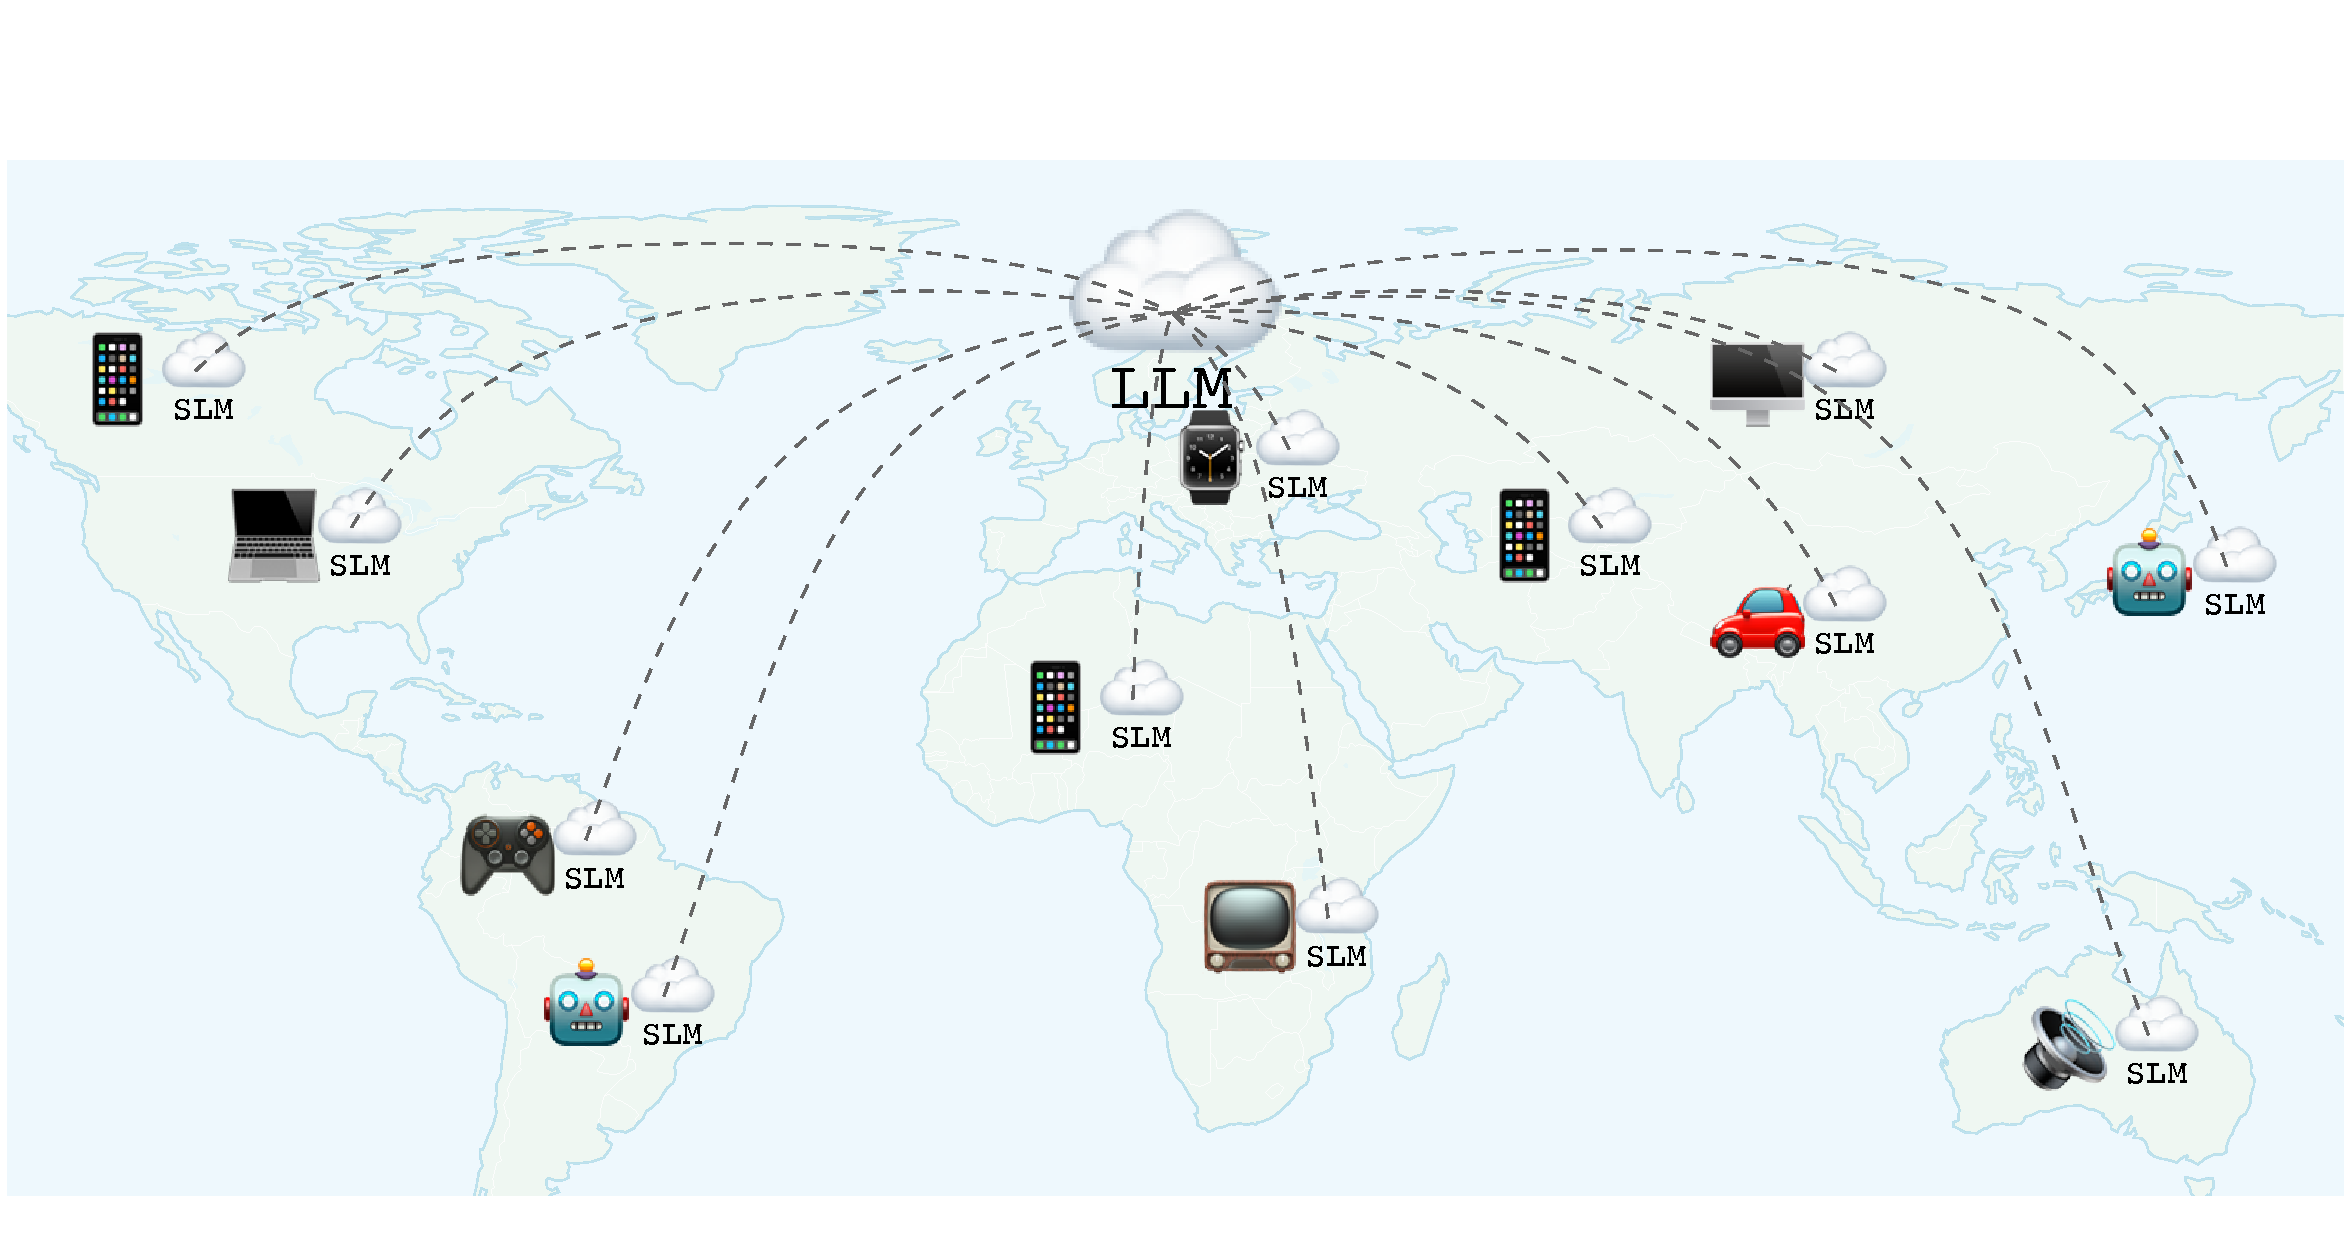
\includegraphics[width=1\linewidth]{./figs/fedllm.pdf}
    \vspace{-20pt}
    \caption{Train Large Language Models with Small Edge Devices}
    \label{fig:fedllm}
\end{figure}
While some federated learning approaches allow training partial model parameters \cite{horvath2021fjord,alam2022fedrolex}, the enormous disparity between large language models and what edge devices can train—often orders of magnitude smaller due to inherently constrained resources—remains too vast to be effectively bridged by current FL frameworks.
Therefore, we need to develop a new federated learning paradigm that enables participants to collaboratively train a large language model even under extremely limited resources (as shown in Figure~\ref{fig:fedllm}).
\textbf{It is still an open problem to train large language models with small edge devices.} Therefore, we encourage the research community to develop novel distributed collaborative computing methods in two key directions:

\subsection{Heterogeneous Device Model Fusion: \\from Small to Large}\label{subsec:model_fusion}

The first direction addresses the fundamental challenge of model size disparity in federated learning. Modern large language models typically contain hundreds of billions of parameters, while edge devices have severely limited computational resources. This creates an enormous scale gap - the large target model may be hundreds or even thousands of times larger than what individual devices can handle. To bridge this gap, each edge device should run a small language model that matches its computational capacity. For example, while the central model may have 100 billion parameters, a resource-constrained mobile device might only handle a 100-million parameter model, representing a 1000x size difference. 
The key challenge then becomes how to effectively aggregate and fuse knowledge from these much smaller models into the large target model. 
We need novel techniques that can meaningfully combine insights from models operating at radically different scales while preserving the unique contributions of each small model. This requires fundamentally rethinking traditional model fusion approaches \citep{velasevic2023effects,azizan2019distributed} to handle such extreme parameter count disparities.

\subsection{Heterogeneous Device Compute Sharing:\\ from Node to Cluster}\label{subsec:compute_sharing}

The second direction is to enable efficient compute resource sharing across heterogeneous devices by treating them as a unified compute cluster rather than independent nodes. Consider a smart home environment where multiple devices—smartphones, laptops, and desktop computers—could form a collaborative compute cluster. While each individual device has limited resources, their collective computing power could be substantial. For example, a laptop could handle intensive computational tasks, smartphones could manage coordination and lightweight processing, and desktop computers could contribute their onboard computing power. Meanwhile, other IoT devices such as smart speakers, security cameras, and vehicles could serve as data sources, providing valuable real-world inputs like voice commands, visual feeds, and environmental parameters. The language model would effectively run and train across this entire device cluster, leveraging both computing power and diverse training data from the environment.
This distributed execution requires new frameworks that can intelligently decompose and distribute model computations based on each device's capabilities and current load. The system must dynamically balance workloads - when the security cameras are idle at night, they could take on additional compute tasks, while during peak usage hours, the load could shift to other devices. 
This requires innovations in real-time resource allocation, task scheduling across heterogeneous hardware, and efficient inter-device communication protocols to ensure the collective computing power is optimally utilized \citep{zhao2024retrieval}.
% to ensure the collective computing power is optimally utilized while maintaining model coherence \citep{zhao2024retrieval}.



% To address the computational limitations of edge devices, several innovative approaches have emerged. Quantization techniques reduce model precision while maintaining performance, enabling efficient computation on resource-constrained devices \cite{zhou2016dorefa}. Similarly, model sparsification and low-rank matrix approximations offer promising directions for reducing computational and memory requirements \cite{wang2020federated}. These techniques, when combined with careful optimization, can significantly reduce the resource footprint of large models while preserving their capabilities.

% In environments characterized by distributed data and asynchronous updates, continuous learning paradigms offer a potential solution. Lifelong learning approaches enable models to adapt and improve over time, even with incomplete or inconsistent updates \cite{chen2018lifelong}. These methods incorporate mechanisms for knowledge retention and transfer, ensuring that new updates do not catastrophically interfere with previously learned information \cite{parisi2019continual}. The integration of meta-learning techniques further enhances the model's ability to adapt to new data distributions and task requirements \cite{finn2017model}.

% Balancing model efficiency and performance during dynamic scaling remains a critical challenge. Adaptive architecture techniques allow models to adjust their capacity based on available resources and task requirements \cite{tan2019efficientnet}. This flexibility enables systems to optimize resource utilization while maintaining performance standards. Furthermore, neural architecture search methods can automatically discover efficient model configurations that are well-suited to distributed training scenarios \cite{zoph2018learning}.

% 5.3 新的问题
% \textbf{Emerging Challenges}
% - 数据异质性如何解决?(各终端设备的数据分布不一致)
% - 如何处理设备异构性与异步更新问题?
% - 在一个持续学习环境中,如何动态调整模型规模?

% \textbf{Data heterogeneity} poses a fundamental challenge in federated learning systems. The non-IID nature of data across different devices can lead to divergent model updates and reduced performance \cite{zhao2018federated}. Recent research has explored techniques such as gradient normalization and personalized models to address these issues \cite{li2020federated}. However, developing robust methods that can handle extreme data heterogeneity while maintaining model performance remains an open challenge.

% \textbf{Device heterogeneity and asynchronous updates} introduce additional complexity to the training process. Variations in device capabilities and availability patterns can lead to inconsistent model updates and training instability \cite{bonawitz2019towards}. Advanced scheduling algorithms and adaptive aggregation methods have been proposed to manage these challenges \cite{yang2019scheduling}, but achieving optimal performance in highly heterogeneous environments remains difficult.

% \textbf{Continuous learning}   The ability to adjust model size and complexity in response to changing requirements and resource constraints is crucial \cite{tan2019efficientnet}. However, this flexibility must be balanced against the need for stable performance and efficient resource utilization. Research in neural architecture search and adaptive computation offers promising directions for addressing these challenges \cite{he2018amc}, but significant work remains to develop robust solutions for production environments.
% \section{Alternative Views}

% While the trend towards training increasingly large models with massive computational resources and data has shown impressive results, there are significant voices in the AI community that challenge this approach. This section presents several key arguments against the "bigger is better" paradigm in AI development.

% \paragraph{Environmental Concerns}
% Training large language models requires enormous amounts of computational power, resulting in significant carbon emissions. For instance, training a GPT-3-sized model can emit as much carbon as several hundred cars in a year \cite{strubell2019energy}. This environmental impact raises serious questions about the sustainability of the current trajectory in AI development.

% \paragraph{Resource Concentration}
% The massive computational and data requirements for training large models create significant barriers to entry, concentrating AI development in the hands of a few well-resourced organizations. This concentration of power leads to limited diversity in AI research and development, reduced competition and innovation in the field, and potential monopolistic control over AI capabilities. The resulting power imbalance threatens to stifle progress and creativity in the AI community.

% \paragraph{Data Quality Over Quantity}
% Critics argue that the focus on massive datasets overlooks the importance of data quality and curation. They emphasize the need for more careful curation of training data, better understanding of data biases and their impacts, and development of methods to learn from smaller, higher-quality datasets. This perspective suggests that improving data quality could be more valuable than simply increasing data quantity.

% % \paragraph{Alternative Research Directions}
% % Several researchers propose alternative approaches to advancing AI capabilities beyond simply scaling up model size. These include focusing on model efficiency and compression techniques, developing more sophisticated architectural innovations, investigating neuromorphic computing and brain-inspired approaches, and exploring few-shot and zero-shot learning capabilities. These alternatives could potentially offer more sustainable paths to AI advancement.

% \paragraph{Ethical and Social Implications}
% The race for larger models raises several ethical concerns that demand careful consideration. These include the potential amplification of biases present in training data, questions about the interpretability and accountability of large models, the broader social impacts of concentrated AI power, and significant privacy concerns regarding the massive data collection required for training. These issues highlight the need for more responsible AI development practices.

% \paragraph{Economic Efficiency}
% Critics question the economic sustainability of the current approach to AI development. High operational costs limit practical applications, while the return on investment for increasingly large models remains questionable. Combined with rising energy costs and extensive infrastructure requirements, these factors point to the need for more cost-effective approaches to AI development that can deliver value while remaining economically viable.

% \textbf{Challenges of edge-generated data.} Despite its promising advantages, edge data presents several significant challenges when utilized for large model pre-training.
% First, while edge data offers superior diversity, its \textbf{heterogeneity} introduces computational complexity. Edge data comes from diverse sources with varying formats and quality standards \cite{seagate_rethinkdata_2020}, requiring sophisticated preprocessing and significantly increasing computational overhead.
% Second, although edge data's real-time capability is advantageous, its \textbf{collection reliability} poses challenges. Edge devices operate in dynamic environments where data quality can be affected by environmental interference and connectivity issues \cite{idc_seagate_dataage_2019}, necessitating robust validation mechanisms.
% Third, edge data's \textbf{distribution characteristic} introduces statistical challenges for model training. Edge nodes generate data following distinct local distributions, complicating the training process as models must learn generalizable patterns. Organizations currently utilize only 57\% of their captured data \cite{seagate_rethinkdata_2020}, highlighting the challenge of effectively incorporating diverse edge distributions.

% To address these challenges, several solutions have been proposed. Advanced data preprocessing techniques can help standardize heterogeneous data sources while preserving their valuable diversity. Robust quality assessment mechanisms can help manage temporal instability while maintaining real-time capabilities. Additionally, federated learning approaches can help balance personalization with generalization, enabling effective utilization of edge-generated data for model pre-training while preserving its unique advantages.

\paragraph{Challenges of edge-generated data} The fundamental challenge in leveraging edge data for large model pre-training lies in its inherent \textit{data heterogeneity}. While edge devices provide access to richer and more diverse data distributions compared to centralized training, managing this heterogeneity has been a core challenge in federated learning \cite {mcmahan2017communication}. The heterogeneity manifests in varying data quality standards, formats, and distinct local statistical distributions that reflect different usage patterns. Fortunately, large language models possess a unique advantage in this context - their significant model capacity and sophisticated architectures allow them to effectively capture and model diverse data distributions simultaneously, making them particularly well-suited for learning from heterogeneous edge data sources.


\paragraph{Challenges of edge computational resources} The fundamental challenge in leveraging edge computing for large model training lies in its inherent \textit{computational heterogeneity}. While edge devices collectively provide massive computing power compared to centralized training, effectively coordinating and utilizing this distributed computing power remains a significant technical challenge \cite{kairouz2021advances}.
The heterogeneity manifests in varying computational capabilities, memory constraints, and distinct resource availability patterns that reflect different device types and usage scenarios. 
To address these challenges, novel distributed training architectures and optimization techniques need to be developed that can effectively handle device heterogeneity while ensuring training efficiency and model quality. This includes adaptive resource allocation strategies, asynchronous training methods, and robust fault tolerance mechanisms.




% 第7章:结论
\section{Conclusion}

In this position paper, we have argued that 
leveraging massive distributed edge devices can break barriers of data and computing wall, and everyone can participate in training large models with small edge devices.
Our comprehensive analysis demonstrated the vast untapped potential of edge resources, with smartphone data volume reaching approximately 33.1 EB and a combined computing power of around 9278 EFLOPS  in the past 5 years. 
These edge resources offer unique advantages in terms of data diversity, privacy, real-time context, and computing efficiency. 
% While significant challenges remain in managing heterogeneity and coordination across distributed systems, 
This paradigm shift towards distributed training could democratize AI development and open an exciting new chapter in the scaling of foundation models.

% In this position paper, we have argued that leveraging massive distributed 
% edge devices can break through current AI development bottlenecks by enabling 
% everyone to participate in training large models with small devices. By 
% analyzing challenges of data depletion and compute monopolization, we 
% demonstrated the vast untapped potential of distributed edge resources. 
% Through examining technical foundations in federated learning and distributed 
% architectures, we showed how these collective resources could democratize AI 
% development and push model scaling boundaries.

% Our analysis of edge computing revealed unique advantages in data diversity, 
% computational capacity, and energy efficiency, though significant challenges 
% remain in managing data heterogeneity and device coordination. The 
% environmental benefits of distributed training are particularly noteworthy, 
% as it eliminates the need for energy-intensive data centers while reducing 
% data transmission costs. Our analysis suggests that this paradigm shift 
% towards distributed training could democratize AI development and open an 
% exciting new chapter in the scaling of foundation models.



% \section*{Accessibility}
% Authors are kindly asked to make their submissions as accessible as possible for everyone including people with disabilities and sensory or neurological differences.
% Tips of how to achieve this and what to pay attention to will be provided on the conference website \url{http://icml.cc/}.

% \section*{Software and Data}

% If a paper is accepted, we strongly encourage the publication of software and data with the
% camera-ready version of the paper whenever appropriate. This can be
% done by including a URL in the camera-ready copy. However, \textbf{do not}
% include URLs that reveal your institution or identity in your
% submission for review. Instead, provide an anonymous URL or upload
% the material as ``Supplementary Material'' into the OpenReview reviewing
% system. Note that reviewers are not required to look at this material
% when writing their review.

% % Acknowledgements should only appear in the accepted version.
% \section*{Acknowledgements}

% \textbf{Do not} include acknowledgements in the initial version of
% the paper submitted for blind review.

% If a paper is accepted, the final camera-ready version can (and
% usually should) include acknowledgements.  Such acknowledgements
% should be placed at the end of the section, in an unnumbered section
% that does not count towards the paper page limit. Typically, this will 
% include thanks to reviewers who gave useful comments, to colleagues 
% who contributed to the ideas, and to funding agencies and corporate 
% sponsors that provided financial support.

% \section*{Impact Statement}

% Authors are \textbf{required} to include a statement of the potential 
% broader impact of their work, including its ethical aspects and future 
% societal consequences. This statement should be in an unnumbered 
% section at the end of the paper (co-located with Acknowledgements -- 
% the two may appear in either order, but both must be before References), 
% and does not count toward the paper page limit. In many cases, where 
% the ethical impacts and expected societal implications are those that 
% are well established when advancing the field of Machine Learning, 
% substantial discussion is not required, and a simple statement such 
% as the following will suffice:

% ``This paper presents work whose goal is to advance the field of 
% Machine Learning. There are many potential societal consequences 
% of our work, none which we feel must be specifically highlighted here.''

% The above statement can be used verbatim in such cases, but we 
% encourage authors to think about whether there is content which does 
% warrant further discussion, as this statement will be apparent if the 
% paper is later flagged for ethics review.


% In the unusual situation where you want a paper to appear in the
% references without citing it in the main text, use \nocite
% \nocite{langley00}
\newpage
\bibliography{example_paper,st,zdd,zzy}
\bibliographystyle{icml2025}


%%%%%%%%%%%%%%%%%%%%%%%%%%%%%%%%%%%%%%%%%%%%%%%%%%%%%%%%%%%%%%%%%%%%%%%%%%%%%%%
%%%%%%%%%%%%%%%%%%%%%%%%%%%%%%%%%%%%%%%%%%%%%%%%%%%%%%%%%%%%%%%%%%%%%%%%%%%%%%%
% APPENDIX
%%%%%%%%%%%%%%%%%%%%%%%%%%%%%%%%%%%%%%%%%%%%%%%%%%%%%%%%%%%%%%%%%%%%%%%%%%%%%%%
%%%%%%%%%%%%%%%%%%%%%%%%%%%%%%%%%%%%%%%%%%%%%%%%%%%%%%%%%%%%%%%%%%%%%%%%%%%%%%%
\newpage
\appendix
\onecolumn
% 逻辑主线: 通过终端设备的协作训练打破垄断,让AI更加普惠和多样化。

% 第6章:广泛影响
\section{Impact Statements}\label{sec:impacts}

The shift from centralized to distributed training of large models, may introduce new technical and societal challenges and have the potential to fundamentally reshape the AI landscape. 

% 6.1 AI垄断与民主化
\subsection{AI Monopoly and Democratization}\label{subsec:ai_monopoly_and_democratization}
% - 终端设备参与训练如何冲击算力垄断?
% - 这种去中心化模式是否有助于普惠性创新?

The current AI landscape is characterized by significant concentration of power among a few tech giants, primarily due to their monopoly over massive computing resources and data centers \cite{bommasani2021opportunities}. This monopolistic trend has intensified with companies like OpenAI increasingly moving towards closed systems. 
While open-source alternatives like Llama \cite{touvron2023llama}, Deepseek \cite{liu2024deepseek} and other community-driven models have made strides towards democratization by releasing model parameters and technical reports \cite{democratizing2024ai}, the gap in computational resources and data access between major AI companies and other players remains substantial and continues to widen. 
This disparity in resources allows tech giants to maintain their absolute dominance in determining the direction of AI development, raising concerns about AI democratization. 


Edge device-based collaborative training presents a promising pathway to democratize AI development \cite{collaborative2024edge}.
By leveraging the collective computing power of millions of edge devices, this approach could effectively challenge the existing monopolistic structure \cite{community2024driven, distributed2024training}. 
This democratization of AI training through edge devices could fundamentally reshape the structure of responsibilities and authorities.
If everyone can participate in training LLMs, the AI landscape could fundamentally change. Training decisions would shift from companies to communities, creating shared responsibility for model development \cite{decentralized2024llm}. Global participation would help models reflect diverse cultural perspectives, while allowing communities to adapt models for their local needs.
Furthermore, this decentralized approach could foster a more competitive and innovative AI ecosystem. When the barriers to entry for AI model training are lowered, we can expect to see a broader range of specialized models emerging (like \cite{domain2024survey,medical2024llm,finance2024gpt,legal2024transformer,science2024llm,education2024transformer}), better suited to local needs and diverse use cases.

% % 6.2 数据隐私
% \subsection{Data Privacy}
% % - 用户个人隐私能否通过联邦学习得到保证?
% % - 隐私保护的机制是否会对模型性能产生影响?

% Privacy preservation is a cornerstone benefit of edge device-based training \cite{bonawitz2017practical}. Through federated learning techniques, users' data remains on their local devices while contributing to model improvement \cite{mcmahan2017communication}. This approach addresses one of the most pressing concerns in AI development - the protection of personal information. The local processing of data eliminates the need for raw data transmission to central servers, significantly reducing privacy risks \cite{truex2019hybrid}.

% While privacy-preserving mechanisms like differential privacy \cite{dwork2014algorithmic} and secure aggregation \cite{bonawitz2017practical} may introduce some computational overhead, research has shown that these trade-offs are often manageable. Modern techniques can maintain model performance while providing strong privacy guarantees, striking a balance between utility and privacy protection \cite{wei2020federated}.

% % 6.3 个人与社会效益
% \subsection{Individual and Social Benefits}
% % - 用户端贡献数据能否获得反哺?(更智能化的服务)
% % - 替代目前集中式模型训练后,AI对社会进步的影响有哪些?

% The distributed training paradigm creates a virtuous cycle where users' contributions to model training directly translate into improved personalized services \cite{wang2019edge}. Users benefit from models that better understand their specific needs and usage patterns, while maintaining control over their data \cite{li2020federated}. This personalization can lead to more efficient and effective AI applications across various domains, from healthcare to education \cite{rieke2020future}.

% From a broader societal perspective, the shift away from centralized training could lead to more equitable access to AI technology \cite{kairouz2021advances}. This democratization could help bridge the digital divide, enabling communities worldwide to develop and deploy AI solutions that address their specific challenges and needs.

% 6.4 公平性与激励机制
\subsection{Fairness and Incentive Mechanisms}\label{subsec:fairness_and_incentive_mechanisms}
% - 讨论分布式训练的模型的公平性?
% - 是否有激励机制吸引用户或设备参与模型训练?

The distributed training paradigm introduces new considerations for model fairness and bias mitigation \cite{yao2024pursuit,li2020fair}. When training occurs across diverse edge devices, the resulting models can potentially better reflect the heterogeneous nature of user populations \cite{wang2020optimizing}. However, this approach also raises concerns about participation bias, where differences in device capabilities or user engagement could lead to underrepresentation of certain groups \cite{kairouz2021advances}. To address these challenges, researchers have proposed various fairness-aware federated learning algorithms \cite{mohri2019agnostic} that aim to ensure equitable model performance across different demographic groups and device types \cite{li2020fair}.

To sustain a distributed training ecosystem, effective incentive mechanisms are crucial for motivating user participation \cite{kang2019incentive}. Traditional approaches like computational resource sharing \cite{khan2019federated} and privacy-preserving reward systems \cite{zhan2020learning} have shown promise in encouraging user engagement. More innovative solutions include token-based reward systems \cite{incentive2024blockchain} and reputation mechanisms \cite{yang2019federated} that compensate users for their contributions while maintaining system integrity. These incentive structures not only encourage consistent participation but also help ensure the quality of contributed training data \cite{feng2019learning}, creating a sustainable ecosystem for collaborative AI development.

\subsection{Carbon Footprint and Energy Efficiency}\label{subsec:carbon_footprint_and_energy_efficiency}
The shift from centralized to distributed training offers compelling environmental benefits \cite{yang2024environmental}. Traditional data centers housing large language models face significant energy challenges\cite{li2024carbon} - their high-performance GPUs require extensive cooling systems that consume 30-40\% of total energy \cite{cooling}. In contrast, FL distributes computation across edge devices like smartphones and tablets that operate at much lower temperatures and power levels, eliminating industrial cooling needs \cite{fl_vs_centralized}.

FL also dramatically reduces data transmission energy costs. While centralized approaches require raw data transfer from millions of devices, FL only transmits lightweight model updates, substantially decreasing network energy overhead \cite{fl_data_transmission}. The hardware efficiency gap is striking - edge devices like the NVIDIA Tegra X2 consume just 7.5W during training compared to 250W for data center GPUs \cite{hardware_power}, translating to major carbon footprint reductions, particularly for simpler models \cite{fl_iid}.
By reducing reliance on power-hungry data centers and leveraging existing consumer devices, FL enables more sustainable AI development through optimized energy efficiency and minimized infrastructure needs. This combination of reduced cooling requirements, efficient hardware utilization, and optimized data handling makes FL an environmentally responsible choice for the future of AI training \cite{fl_environmental}. As climate impact becomes increasingly critical, FL's sustainability advantages position it as a key technology for green AI development.

% 逻辑主线: 梳理现有AI发展依赖的关键要素和遇到的瓶颈,论述为什么海量小设备可以成为未来突破点。

% 第2章:大语言模型是AI发展的历史性成功
\section{Historical Development and Current Challenges}\label{sec:history}
% - 大语言模型是AI发展的历史性成功

% 2.1 大模型成功的驱动力: Scaling Law
% \subsection{Scaling law: the compass for LLMs}
% - 什么是Scaling Law?
% - 图2.1来说明Scaling Law,大模型的参数,以及训练所需的数据量、算力和越来越大,比如从BERT到GPT-4
% - Scaling Law为什么推动了大模型的成功?(模型/数据的扩张如何保障性能提高?)
% - 数据、模型、算力的扩张之间的关系。

% 2.2 海量数据是大模型成功的核心原因
\subsection{Data: the fuel of LLMs}

\paragraph{Early data-driven AI development}
As LLMs continue to achieve unprecedented success in artificial intelligence, understanding the role of data becomes increasingly crucial. From the early days of simple datasets to the modern era of massive data collections, data has consistently served as the lifeblood of AI, determining the upper bounds of model capabilities. The evolution of AI—marked by breakthroughs in computer vision, natural language processing, and beyond—can be traced back to the continuous expansion and refinement of data resources. 

In the early stages of AI, despite relatively small data scales, the importance of data was already evident. The MNIST dataset, for instance, serves as a notable example. With 60,000 training images and 10,000 test images, it provided a crucial foundation for neural network research, demonstrating the fundamental role of data in model training~\cite{lecun1998mnist}. As data scales expanded, the capabilities of deep learning models saw significant improvements. The emergence of ImageNet, which contains 14 million images across 21,000 synsets, revolutionized computer vision. This enabled deep learning models like AlexNet to learn complex visual features and achieve breakthrough progress in image recognition tasks, reducing error rates from 26.2\% to 15.3\% in the ILSVRC-2012 competition~\cite{deng2009imagenet,krizhevsky2012imagenet}. ImageNet's success stemmed not only from its scale but also from its high quality and diversity, laying the groundwork for subsequent large-scale data applications.

\paragraph{Era of massive data}
With the proliferation of the internet and advances in computing power, data scales have expanded dramatically, ushering AI into an era of massive data. GPT-3, for instance, was trained on 450 billion tokens, with a carefully curated mix of data sources: Common Crawl (60\%), books (16\%), Wikipedia (3\%), and other internet-based text (21\%)~\cite{brown2020language}. This massive dataset enabled GPT-3 to excel across various tasks, demonstrating the decisive role of data scale in model capabilities. Compared to early datasets like MNIST and ImageNet, GPT-3's data scale and quality reached unprecedented heights, not only advancing natural language processing but also opening new possibilities for AI generalization.

\paragraph{Quality and diversity matter}
Beyond scale, data quality and diversity are crucial factors in model performance. ImageNet ensures data quality through rigorous validation, with each image verified by an average of 3.3 annotators and achieving 95\% accuracy in its labels~\cite{deng2009imagenet}. This precise annotation enables models to learn accurate visual features and excel in image classification tasks. In the realm of large language models, GPT-3's training data underwent stringent cleaning and filtering, including deduplication, quality scoring based on document length and linguistic complexity, and content filtering for inappropriate content~\cite{brown2020language}. This high-quality data enables GPT-3 to generate coherent and accurate text. Furthermore, diversity is essential: ImageNet covers 1,000 object categories across various domains, while GPT-3's training data spans multiple languages, genres, and knowledge domains, providing rich linguistic knowledge and contextual understanding.

\paragraph{Data as the ceiling for model capabilities}
A model's capability depends on the knowledge it extracts from data, following empirically observed scaling laws. While increasing model parameters can enhance expressive power, without sufficient data, models cannot effectively utilize these parameters. DeepMind's research on the Chinchilla model demonstrated that under the same compute budget, a 70B parameter model trained on 1.4T tokens outperforms a 280B parameter model trained on 0.35T tokens, achieving a 30\% reduction in loss while using the same compute resources~\cite{hoffmann2022training}. This finding directly supports the notion that data acts as a ceiling for model capabilities. Additionally, Meta's research shows that while Llama 2 (70B) has 70 billion parameters, its performance largely benefits from training on 2T tokens of high-quality data, with particular emphasis on academic papers, code repositories, and books that enhance its reasoning capabilities~\cite{touvron2023llama}. These studies emphasize data's central role in model training and suggest that optimal model scaling requires a balanced increase in both parameters and training data.

\paragraph{Looking ahead}
From MNIST to ImageNet to GPT-3, advances in data scale, quality, and diversity have directly driven AI breakthroughs. Data remains the foundation of AI development, determining the upper limits of model capabilities. As we push the boundaries of LLM performance, the challenge of acquiring sufficient high-quality, diverse data becomes increasingly acute. Traditional data sources like the internet are showing signs of exhaustion, and concerns about data privacy and ownership are growing. This motivates the exploration of novel data acquisition approaches, such as leveraging edge devices and distributed data collection, which we will explore in subsequent sections. The future of LLMs may depend not just on scaling existing data sources, but on fundamentally rethinking how we collect, curate, and utilize data in AI training.

% 2.3 大模型的训练需要超大算力支撑
\subsection{Computing power: the engine of LLMs}
% - 历史上算力的提升如何推动AI的突破?
% - 算力发展的历史(从CPU到GPU到TPU,从单卡到多卡到集群)
% - 图2.1解释所需算力不断增大(从BERT到GPT-4需要算力的变化)
% - AI的每次进步都是靠算力支撑。
\paragraph{Early neural networks and CPU era}
Since the inception of neural networks, every breakthrough in the field of AI has been driven by the continuous improvement of computational power~\cite{thompson2020computational}. From the early multilayer perceptron (MLP) to the widely used large language models (LLM) today, the progress in computing power has always been a key engine for advancing AI.

As the prototype of neural networks, the MLP was initially used to solve linearly separable problems~\cite{rosenblatt1958perceptron}. Due to its relatively low computational demand, it could run on traditional CPU environments. However, as the complexity of neural network models increased and application scenarios expanded, computational requirements gradually rose. The emergence of Convolutional Neural Networks (CNN) and Recurrent Neural Networks (RNN) marked a surge in computational demands. CNN, through convolutional operations, effectively reduced the number of parameters, enhancing the computational efficiency of image processing tasks. Classic models such as LeNet~\cite{lecun1998gradient} and AlexNet~\cite{krizhevsky2012imagenet} achieved significant results in image classification, but this also led to a surge in computational resource demands. For example, AlexNet's victory in the 2012 ImageNet competition was made possible by using the NVIDIA GTX 580 GPU, which significantly boosted computational performance~\cite{krizhevsky2012imagenet}.

\paragraph{GPU and TPU revolution}
With the growing scale of neural network models, GPUs gradually became indispensable computing tools~\cite{raina2009large}. The parallel computing capabilities of GPUs greatly accelerated the training process of neural networks, particularly in the field of deep learning. Meanwhile, specialized hardware for deep learning, such as Tensor Processing Units (TPUs), emerged~\cite{jouppi2017datacenter}. Compared to GPUs, TPUs offer higher efficiency and lower power consumption when performing matrix operations and deep learning tasks~\cite{wang2019benchmarking}, making them the preferred hardware for training large-scale neural networks.

\paragraph{Transformer era and computational demands}
As computational resources continued to expand, the scale of neural network model training also grew. The introduction of the Transformer architecture~\cite{vaswani2017attention} revolutionized the field of natural language processing (NLP), especially with the launch of models like BERT~\cite{devlin2018bert} and the GPT series~\cite{brown2020language,openai2023gpt4}, which pushed NLP technology to new heights. However, the self-attention mechanism in the Transformer architecture has a computational complexity of $O(n^2)$, where n represents the sequence length~\cite{vaswani2017attention}. This means that as the model scale and sequence length increase, the required computational power grows exponentially. For example, training large language models like GPT-3~\cite{brown2020language} and GPT-4~\cite{openai2023gpt4} involves trillions of parameters and requires thousands of GPUs or TPU nodes to support the process. This immense computational demand not only places extremely high requirements on hardware, but also on computational frameworks, storage, and communication bandwidth, creating unprecedented challenges~\cite{patterson2021carbon}.

\paragraph{Computing power as the key driver}
Every leap in Artificial Intelligence has been driven by computational power~\cite{amodei2018ai}. From multilayer perceptrons to convolutional neural networks, and the introduction of the Transformer architecture, every innovation in models has been accompanied by an explosive growth in computational needs~\cite{thompson2020computational}. Particularly in the era of large language models, computational power is not only the foundational tool for model training but also the core driving force behind breakthroughs in AI performance~\cite{kaplan2020scaling}. The success of large-scale models like GPT-4 validates that AI progress almost entirely depends on the support of more powerful computational resources~\cite{hoffmann2022training}.



\section{Smartphone Data Volume Estimation}  
\label{app:smartphone_ethod}

In the absence of publicly available, granular data on per-user smartphone data generation patterns, we adopt a conservative estimation approach to approximate the total annual smartphone data volume. While this method necessarily involves simplifications, it provides a robust lower-bound approximation that is sufficient to support our core arguments without compromising the validity of our conclusions.

\textbf{Data volume estimation per smartphone}: Based on industry reports  \cite{counterpoint_smartphone_2021}, the average smartphone storage capacity reached 100 GB in 2020. To ensure a conservative estimate, we assume that only 1\% of this storage capacity (equivalent to approximately 1 GB per smartphone) is actively used for data generation and storage, including local images, video information, and other types of user-generated content. This assumption aligns with baseline usage scenarios while intentionally underestimating actual data utilization.
    % \item \textbf{Static Data Generation}: For simplicity, we adopt a static model that assumes no incremental data generation beyond this initial 1 GB allocation per device. This approach disregards dynamic factors such as daily usage patterns, application updates, or video/photo storage, thereby providing a conservative lower bound for smartphone data volume.

\textbf{Number of smartphones}: The growth of the number of smartphone users is an important basis for estimating the total amount of data. For this, we have referred to data from market research institutions \cite{bankmycell_smartphone_2023}, which includes trends in changes to the number of smartphone users over time.


Based on the above statistical data, the total annual smartphone data volume \( D_{\text{total}} \) is calculated using the following formula:  
\begin{equation}  
    D_{\text{total}}  (\text{EB}) = N_{\text{users}} \times 1 \, \text{GB/user} \times 10^{-3}  \, (\text{conversion from GB to EB}),
\end{equation}  
where \( N_{\text{users}} \) represents the global smartphone user base in billions.  

Substituting \( N_{\text{users}} = 8.0 \times 10^9 \) (representing 8 billion users) into Equation (1):  
\begin{equation*}  
    D_{\text{total}} = 8.0 \, \text{GB/user} \times 10^{-3} = 8.0 \, \text{EB}.
\end{equation*}  

Our purpose is to establish a defensible lower bound for analysis. Even under these stringent assumptions, the derived volumes remain orders of magnitude higher than synthetic or centralized datasets, thereby reinforcing the strategic importance and value of edge-generated data. This conservative estimation underscores the critical need for scalable solutions capable of managing and leveraging such vast quantities of distributed data effectively.  


\begin{table}[h!]
\centering
\caption{Trends in Smartphone Shipments and Compute Power. (Data source: \cite{canalys2025}).}
\label{tab:chip_total}
\resizebox{.95\linewidth}{!}{%
\begin{tabular}{cccc}
\hline
\textbf{Company} & \textbf{Shipments (Million units)} & \textbf{Chip Performance Range (TFLOPS)} & \textbf{Total Compute Power Contribution (EFLOPS)} \\
\hline
\multicolumn{4}{c}{\textbf{2020}} \\ \hline
Samsung (20\%) & 255.5 & 1.20--1.53 & 349 \\
Apple (16\%)   & 207.2 & 0.65 & 135 \\
Xiaomi (12\%)  & 149.6 & 0.24--1.20 & 108 \\
OPPO (9\%)    & 119.4 & 0.24--1.20 & 86 \\
vivo (9\%)    & 112.6 & 0.24--1.20 & 81 \\
Others (33\%)  & 420.5 & 0.04--0.24 & 59 \\ \hline
\multicolumn{4}{c}{\textbf{Overall: Shipments = 1265 Million, Compute Power = 817 EFLOPS}} \\ \hline \hline

\multicolumn{4}{c}{\textbf{2021}} \\ \hline
Samsung (20\%) & 274.5 & 1.42--1.72 & 430 \\
Apple (17\%)   & 230.1 & 1.71--1.94 & 420 \\
Xiaomi (14\%)  & 191.2 & 0.82--1.74 & 240 \\
OPPO (11\%)    & 145.1 & 0.82--1.74 & 180 \\
vivo (10\%)    & 129.9 & 0.82--1.74 & 160 \\
Others (28\%)  & 379.4 & 0.27--0.82 & 207 \\ \hline
\multicolumn{4}{c}{\textbf{Overall: Shipments = 1350 Million, Compute Power = 1637 EFLOPS}} \\ \hline \hline

\multicolumn{4}{c}{\textbf{2022}} \\ \hline
Samsung (22\%) & 257.9 & 0.49--2.01 & 322 \\
Apple (19\%)   & 232.2 & 1.79 & 416 \\
Xiaomi (13\%)  & 152.7 & 1.01--3.49 & 351 \\
OPPO (10\%)    & 113.4 & 1.01--3.49 & 261 \\
Transsion (6\%)     & 73.1 & 0.24--0.98 & 44.6 \\
Others (31\%)  & 364.1 & 0.84--1.31 & 393 \\ \hline
\multicolumn{4}{c} {\textbf{Overall: Shipments = 1193 Million, Compute Power = 1788 EFLOPS}} \\ \hline \hline

\multicolumn{4}{c}{\textbf{2023}} \\ \hline
Apple (20\%)   & 229.1 & 2.15 & 493 \\
Samsung (20\%) & 225.5 & 2.01--2.77 & 539 \\
Xiaomi (13\%)  & 146.1 & 2.15--3.99 & 449 \\
OPPO (9\%)     & 100.7 & 2.15--3.99 & 309 \\
Transsion (8\%)  & 92.6 & 0.24--1.31 & 72 \\
% vivo (7.6\%)  & 87.0 & 2.15--3.99 & 267 \\
Others (30\%)  & 347.9 & 0.24--2.15 & 416 \\
\hline
\multicolumn{4}{c}{\textbf{Overall: Shipments = 1142 Million, Compute Power = 2278 EFLOPS}} \\ \hline \hline

\multicolumn{4}{c}{\textbf{2024}} \\ \hline
Apple (18\%)   & 225.9 & 1.91--2.29 & 474 \\
Samsung (18\%) & 222.9 & 3.38--3.41 & 758 \\
Xiaomi (14\%)  & 168.6 & 3.38--4.95 & 703 \\
Transsion (9\%)  & 106.7 & 0.05--0.67 & 38  \\
OPPO (8\%)   & 103.6 & 3.38--4.95 & 432 \\
Others (33\%)  & 395.4 & 0.05--1.72 & 352 \\
\hline
\multicolumn{4}{c}{\textbf{Overall: Shipments = 1223 Million, Compute Power = 2758 EFLOPS}} \\ \hline
\end{tabular}%
}
\end{table}

\section{Estimation of Smartphone Total Computational Power}  
\label{app:total_computation}

To assess the (ideally) aggregate computational capabilities of smartphones globally, we estimate the total computing power, given the current lack of comprehensive statistical data in this domain. Our approach leverages two key data sources: the annual worldwide shipment volumes for major smartphone brands, and the computational performance specifications of mobile processors deployed in their devices during each corresponding year. The complete data underlying our analysis is presented in Table~\ref{tab:chip_total}, which provides a detailed breakdown by manufacturer and time period.
For quantitative analysis, we formulated a mathematical model to calculate the total computing power. Specifically, for any given year, we compute the aggregate computational capacity ($C_{\text{total}}$) by summing the contributions from each smartphone manufacturer ($i$). Each manufacturer's contribution is determined by multiplying their total device shipments ($N_i$) by the average computing power of their mobile processors ($P_i$) for that year, expressed formally as:

\begin{equation}
    C_{\text{total}} = \sum_{i} N_i \cdot P_i
\end{equation}

This formulation enables us to systematically track the evolution of distributed computing power across the smartphone ecosystem while accounting for both market share dynamics and technological advancement in mobile processors. By maintaining conservative estimates for processor capabilities and focusing on verified shipment data, our analysis provides a reliable lower bound for the total computational resources available through smartphones.

\section{Small Language Model (SLM) Architectures and Training Methods}
\label{app:slm_architectures_training}

Table~\ref{tab:slm_architectures_training} presents a comprehensive overview of the Small Language Model (SLM) landscape, categorized by architectures and training methodologies, according to \citet{wang2024comprehensive}. The table is organized into two main categories: (I) Transformer-Based Models, which represent the dominant architecture in current SLMs, and (II) Alternative Architecture Models, which explore novel approaches to achieve efficiency. The Transformer-Based section is further divided into models pre-trained from scratch, models derived from larger LLMs through knowledge distillation, and models created through various compression techniques (pruning, quantization, etc.). The Alternative Architecture section showcases emerging approaches like State Space Models (Mamba, Hymba), recurrent architectures (RWKV, xLSTM), and traditional encoder-decoder or encoder-only designs. 


\begin{table}[h!]
    \caption{Small Language Model (SLM) Architectures and Training Methods}
    \label{tab:slm_architectures_training}
    \tiny
    \begin{tabularx}{\textwidth}{p{2.5cm}p{1.5cm}p{1.5cm}ccp{2.5cm}p{3cm}}
    \toprule
    \textbf{Model} & \textbf{Sizes} & \textbf{Architecture} & \textbf{From Scratch} & \textbf{From LLMs} & \textbf{Training Method} & \textbf{Datasets} \\
    \midrule
    
    \multicolumn{7}{l}{\textbf{\textit{I. Transformer-Based Models}}} \\
    \midrule
    
    \multicolumn{7}{l}{\textit{I.A. Pre-Trained from Scratch}} \\
    \addlinespace[0.5ex]
    PhoneLM \cite{yi2024phonelm} & 0.5B; 1.5B & Transformer & \checkmark & & Pre-training & DCLM-baseline \cite{li2024datacomp}, StarCoderData \cite{li2023starcodersourceyou} \\
    Llama 3.2 \cite{llama3.2} & 1B; 3B & Transformer & \checkmark & & Pre-training, SFT, RLHF, DPO & Not released (9T tokens) \\
    Qwen 1/1.5/2/2.5 \cite{yang2024qwen2, bai2023qwentechnicalreport} & 0.5B-7B & Transformer & \checkmark & & Pre-training & Not released \\
    Gemma/Gemma 2 \cite{team2024gemma, team2024gemma2} & 2B; 7B & Transformer & \checkmark & & Pre-training & Unknown \\
    SmolLM \cite{allal2024SmolLM} & 135M-1.7B & Transformer & \checkmark & & Pre-training & SmolLM corpus \cite{benallal2024smollmcorpus} \\
    H2O-Danube3 \cite{pfeiffer2024h2o} & 500M; 4B & Transformer & \checkmark & & Pre-training (multi-stage) & Unknown \\
    MiniCPM \cite{hu2024minicpm} & 1.2B; 2.4B & Transformer & \checkmark & & Pre-training & Dolma \cite{dolma}, C4 \cite{raffel2020exploring} \\
    CT-LLM \cite{du2024chinesetinyllmpretraining} & 2B & Transformer & \checkmark & & Pre-training & MAP-CC \\
    OLMo \cite{groeneveld2024olmo} & 1B; 7B & Transformer & \checkmark & & Pre-training & Dolma \cite{dolma} (multiple sources) \\
    TinyLlama \cite{zhang2024tinyllamaopensourcesmalllanguage} & 1B & Transformer & \checkmark & & Pre-training & SlimPajama \cite{cerebras2023slimpajama} \\
    Phi-series \cite{abdin2024phi, javaheripi2023phi} & 1.3B-6.6B & Transformer & \checkmark & & Pre-training & CodeTextBook \cite{gunasekar2023textbooksneed} \\
    OpenELM \cite{mehta2024openelm} & 270M-3B & Transformer & \checkmark & & Pre-training & RefinedWeb \cite{penedo2023refinedweb}, PILE \cite{gao2020pile} \\
    MobiLlama \cite{thawakar2024mobillama} & 0.5B; 0.8B & Transformer & \checkmark & & Pre-training & LLM360 Amber \\
    MobileLLM \cite{liu2024mobilellm} & 125M; 350M & Transformer & \checkmark & & Pre-training & Unknown (1T tokens) \\
    \addlinespace[0.5ex]
    
    \midrule
    \multicolumn{7}{l}{\textit{I.B. Derived from Larger Models}} \\
    \addlinespace[0.5ex]
    MINITRON \cite{muralidharan2024compact} & 4B & Transformer & & \checkmark & Distillation, Pruning & 8T tokens from Nemotron-4 \\
    Orca/Orca 2 \cite{mitra2023orca, mukherjee2023orca} & 7B; 13B & Transformer & & \checkmark & Distillation & Orca 2 dataset, FLAN-v2 \cite{longpre2023flan} \\
    MINIMA \cite{zhang2023towards} & 3B & Transformer & & \checkmark & Distillation (from Llama-2-7B) & Pile \cite{gao2020pile}, Wudao \\
    Dolly-v2 \cite{DatabricksBlog2023DollyV2} & 3B; 7B & Transformer & & \checkmark & Instruction tuning (from Pythia) & Databricks-dolly-15k \\
    LaMini-LM \cite{wu-etal-2024-lamini} & 61M-7B & Transformer & & \checkmark & Distillation & LaMini instruction dataset \\
    \addlinespace[0.5ex]

    \midrule
    \multicolumn{7}{l}{\textit{I.C. Model Compression Approaches}} \\
    \addlinespace[0.5ex]
    SparseGPT \cite{frantar2023sparsegpt} & Various & Transformer & & \checkmark & Unstructured Pruning & Not applicable \\
    Wanda \cite{sun2024a} & Various & Transformer & & \checkmark & Unstructured Pruning & Not applicable \\
    LoRAPrune \cite{zhang2023loraprune} & Various & Transformer & & \checkmark & Unstructured Pruning & Not applicable \\
    ShortGPT \cite{men2024shortgpt} & Various & Transformer & & \checkmark & Structured Pruning & Not applicable \\
    BitNet/BitNet b1.58 \cite{wang2023bitnet, ma2024era} & Various & Transformer & & \checkmark & Quantization (QAT) & Not applicable \\
    QLoRA \cite{dettmers2024qlora} & Various & Transformer & & \checkmark & Quantization, Low-Rank & Various fine-tuning datasets \\
    SqueezeLLM \cite{kim2023squeezellm} & Various & Transformer & & \checkmark & Quantization (PTQ) & Not applicable \\
    \midrule
    
    \multicolumn{7}{l}{\textbf{\textit{II. Alternative Architecture Models}}} \\
    \midrule
    
    % \multicolumn{7}{l}{\textit{II.A. State Space Models and RNNs}} \\
    \addlinespace[0.5ex]
    Mamba \cite{gu2023mamba} & 125M-1.3B & Mamba & \checkmark & & Pre-training & Pile \cite{gao2020pile} \\
    Rene \cite{Rene} & 1.3B & Mamba & \checkmark & & Pre-training & Dolma-1.7 \cite{dolma} \\
    Zamba2 \cite{glorioso2024zambacompact7bssm} & 2.7B & Mamba & \checkmark & & Pre-training & Not specified \\
    Hymba \cite{dong2024hymba} & 125M-1.5B & Hymba & \checkmark & & Pre-training & DCLM-Baseline \cite{li2024datacomp} \\
    xLSTM \cite{beck2024xlstm} & 125M-1.3B & xLSTM & \checkmark & & Pre-training & SlimPajama \cite{cerebras2023slimpajama} \\
    RWKV \cite{peng-etal-2023-rwkv} & 169M-14B & RNN & \checkmark & & Pre-training & Pile \cite{gao2020pile} \\
    \addlinespace[0.5ex]
    
    % \multicolumn{7}{l}{\textit{II.B. Encoder-Decoder Models}} \\
    \addlinespace[0.5ex]
    Specialized FlanT5 \cite{fu2023specializing} & 250M-3B & Encoder-Decoder & & \checkmark & Instruction Tuning & GSM8K \cite{cobbe2021gsm8k} \\
    FlanT5 \cite{chung2024scaling} & 80M-3B & Encoder-Decoder & & \checkmark & Instruction Tuning & Muffin, T0-SF, SNI and CoT \\
    T5 \cite{raffel2020exploring} & 60M-3B & Encoder-Decoder & \checkmark & & Pre-training & C4 \cite{raffel2020exploring} \\
    \addlinespace[0.5ex]
    
    % \multicolumn{7}{l}{\textit{II.C. Encoder-Only Models}} \\
    \addlinespace[0.5ex]
    DistilBERT \cite{sanh2019distilbert} & 66M & Encoder-only & & \checkmark & Distillation (from BERT) & Wikipedia, BookCorpus \\
    TinyBERT \cite{jiao2020tinybert} & 14.5M & Encoder-only & & \checkmark & Distillation (from BERT) & Wikipedia, BookCorpus \\
    ALBERT \cite{lan2020albert} & 12M-18M & Encoder-only & \checkmark & & Pre-training (parameter sharing) & Wikipedia, BookCorpus \\
    \bottomrule
    \end{tabularx}
    \end{table}

    This classification showcases the architectural innovations and training methodologies that are driving the SLM field forward, providing essential technical foundations for deploying powerful AI capabilities on resource-constrained edge devices. By documenting various model sizes, training corpora, and development techniques, the table offers a comprehensive overview of cutting-edge approaches that enable sophisticated language processing directly on end-user devices. These advancements represent critical building blocks for the next generation of on-device AI systems that can operate efficiently without constant cloud connectivity while still delivering robust performance across diverse applications.



\section{Distributed Collaborative Frameworks}
\label{app:distributed_collaborative_frameworks}
Distributed collaborative frameworks enable the deployment, training, and fine-tuning of language models across multiple devices or servers. Table \ref{tab:framework_comparison} presents a comparison of prominent frameworks in this domain. These frameworks can be broadly categorized into three types: cloud-based platforms that offer centralized resources for distributed computing, federated learning systems that enable training across decentralized data sources while preserving privacy, and fully decentralized frameworks that distribute computation across peer nodes. Some frameworks like Neurosurgeon \cite{kang2017neurosurgeon}, MoE$^2$ \cite{jin2025moe2}, Edgent \cite{li2018edgent}, and Galaxy \cite{ye2024galaxy} focus on collaborative inference by partitioning models between edge devices and servers. Others, such as FedLLM \cite{wu2024fedllm}, FedFM \cite{chen2024fedfm}, FedPET \cite{li2024fedpet}, and Photon \cite{sani2024photon}, specialize in federated fine-tuning of large language models while maintaining data privacy. These frameworks are essential for enabling efficient deployment of language models in resource-constrained environments and for scenarios requiring privacy preservation or operation in disconnected settings.

\begin{table}[h!]
    \centering
    \setlength{\tabcolsep}{2pt}
    \begin{tabular}{l*{7}{c}}
    \toprule
    & \multicolumn{4}{c}{\textbf{Distributed Capabilities}} & & & \\
    \cmidrule(lr){2-5}
    \textbf{Framework} & \textbf{Inference} & \textbf{Training} & \textbf{Pretraining} & \textbf{Fine-tuning} & \textbf{Type} & \textbf{Privacy} & \textbf{License} \\
    \midrule
    exo-explore/exo \cite{exo} & \checkmark &  &  &  & Decentralized &  & MIT \\
    Together AI \cite{together} & \checkmark & \checkmark & \checkmark & \checkmark & Cloud &  & Commercial \\
    FLock Platform \cite{flock} &  & \checkmark &  & \checkmark & Federated, Blockchain & \checkmark & Apache 2.0  \\
    OpenDiloco \cite{OpenDiLoCo} &  & \checkmark & \checkmark &  & Decentralized &  & Apache 2.0 \\
    FederatedScope \cite{federatedscope} &  & \checkmark &  & \checkmark & Federated & \checkmark & Apache 2.0 \\
    FedML \cite{fedml} &  & \checkmark &  & \checkmark & Federated & \checkmark & Apache 2.0 \\
    Flower \cite{Flower} &  & \checkmark &  & \checkmark & Federated & \checkmark & Apache 2.0 \\
    FATE-LLM \cite{fan2023fate} &  & \checkmark &  & \checkmark & Federated & \checkmark & Apache 2.0 \\
    FedLLM \cite{ye2025fedllm} &  & \checkmark & \checkmark & \checkmark & Federated & \checkmark & CC BY-NC 4.0 \\
    \bottomrule
    \end{tabular}
    \caption{Comparison of Distributed Machine Learning Frameworks}
    \label{tab:framework_comparison}
\end{table}

% \section{You \emph{can} have an appendix here.}

% You can have as much text here as you want. The main body must be at most $8$ pages long.
% For the final version, one more page can be added.
% If you want, you can use an appendix like this one.  

% The $\mathtt{\backslash onecolumn}$ command above can be kept in place if you prefer a one-column appendix, or can be removed if you prefer a two-column appendix.  Apart from this possible change, the style (font size, spacing, margins, page numbering, etc.) should be kept the same as the main body.
%%%%%%%%%%%%%%%%%%%%%%%%%%%%%%%%%%%%%%%%%%%%%%%%%%%%%%%%%%%%%%%%%%%%%%%%%%%%%%%
%%%%%%%%%%%%%%%%%%%%%%%%%%%%%%%%%%%%%%%%%%%%%%%%%%%%%%%%%%%%%%%%%%%%%%%%%%%%%%%


\end{document}


% This document was modified from the file originally made available by
% Pat Langley and Andrea Danyluk for ICML-2K. This version was created
% by Iain Murray in 2018, and modified by Alexandre Bouchard in
% 2019 and 2021 and by Csaba Szepesvari, Gang Niu and Sivan Sabato in 2022.
% Modified again in 2023 and 2024 by Sivan Sabato and Jonathan Scarlett.
% Previous contributors include Dan Roy, Lise Getoor and Tobias
% Scheffer, which was slightly modified from the 2010 version by
% Thorsten Joachims & Johannes Fuernkranz, slightly modified from the
% 2009 version by Kiri Wagstaff and Sam Roweis's 2008 version, which is
% slightly modified from Prasad Tadepalli's 2007 version which is a
% lightly changed version of the previous year's version by Andrew
% Moore, which was in turn edited from those of Kristian Kersting and
% Codrina Lauth. Alex Smola contributed to the algorithmic style files.
